%%%%%%%%%%%%%%%%%%%%%%%%%%%%%%%%%%%%%%%%%
% Classicthesis Typographic Thesis
% LaTeX Template
% Version 1.4 (1/1/16)
%
% This template has been downloaded from:
% http://www.LaTeXTemplates.com
%
% Original author:
% André Miede (http://www.miede.de) with commenting modifications by:
% Vel (vel@LaTeXTemplates.com)
%
% License:
% GNU General Public License (v2)
%
% General Tips:
% 1) Make sure to edit the classicthesis-config.file
% 2) New enumeration (A., B., C., etc in small caps): \begin{aenumerate} \end{aenumerate}
% 3) For margin notes: \marginpar or \graffito{}
% 4) Do not use bold fonts in this style, it is designed around them
% 5) Use tables as in the examples
% 6) See classicthesis-preamble.sty for useful commands
%
%%%%%%%%%%%%%%%%%%%%%%%%%%%%%%%%%%%%%%%%%

%----------------------------------------------------------------------------------------
%	PACKAGES AND OTHER DOCUMENT CONFIGURATIONS
%----------------------------------------------------------------------------------------

\documentclass[
		oneside,openright,titlepage,numbers=noenddot,headinclude,%1headlines,
	 	footinclude=false,cleardoublepage=empty,
		dottedtoc, % Make page numbers in the table of contents flushed right with dots leading to them
		BCOR=5mm,paper=a4,fontsize=11pt, % Binding correction, paper type and font size
		ngerman,american, % Languages, change this to your language(s)
		]{scrreprt} 
                
% Includes the file which contains all the document configurations and packages - make sure to edit this file
%%%%%%%%%%%%%%%%%%%%%%%%%%%%%%%%%%%%%%%%%
% Classicthesis Typographic Thesis
% Configuration File
%
% This file has been downloaded from:
% http://www.LaTeXTemplates.com
%
% Original author:
% André Miede (http://www.miede.de) with extensive commenting changes by:
% Vel (vel@LaTeXTemplates.com)
%
% License:
% GNU General Public License (v2)
%
% Important note:
% The main lines to change in this file are in the DOCUMENT VARIABLES
% section, the rest of the file is for advanced configuration.
%
%%%%%%%%%%%%%%%%%%%%%%%%%%%%%%%%%%%%%%%%%

%----------------------------------------------------------------------------------------
%	CHARACTER ENCODING
%----------------------------------------------------------------------------------------

\PassOptionsToPackage{utf8}{inputenc} % Set the encoding of your files. UTF-8 is the only sensible encoding nowadays. If you can't read äöüßáéçèê∂åëæƒÏ€ then change the encoding setting in your editor, not the line below. If your editor does not support utf8 use another editor!
\usepackage{inputenc}

%----------------------------------------------------------------------------------------
%	DOCUMENT VARIABLES
%	Fill in the lines below to enter your information into the thesis template
%	Each of the commands can be cited anywhere in the thesis
%----------------------------------------------------------------------------------------

% Remove drafting to get rid of the '[ Date - classicthesis version 4.0 ]' text at the bottom of every page
\PassOptionsToPackage{eulerchapternumbers,listings,drafting, pdfspacing, subfig,beramono,eulermath,parts}{classicthesis}
% Available options: drafting parts nochapters linedheaders eulerchapternumbers beramono eulermath pdfspacing minionprospacing tocaligned dottedtoc manychapters listings floatperchapter subfig

\newcommand{\myTitle}{Modeling and Control of McKibben Artificial Muscle -- Application of Model Predictive Control and Genetic Algorithms\xspace}
\newcommand{\mySubtitle}{}
\newcommand{\myDegree}{Master's Degree in Computer and Systems Engineering}
\newcommand{\myName}{Michele Iessi}
\newcommand{\myProf}{Costanzo Manes\xspace}
\newcommand{\myOtherProf}{Put name here\xspace}
\newcommand{\mySupervisor}{Kazuhisa Ito\xspace}
\newcommand{\myFaculty}{\xspace}
\newcommand{\myDepartment}{Department of Information Engineering, Computer Science and Mathemtics\xspace}
\newcommand{\myUni}{University of L'Aquila\xspace}
\newcommand{\myLocation}{L'Aquila, Italy\xspace}
\newcommand{\myTime}{January 2019\xspace}
\newcommand{\myVersion}{version 0.1\xspace}

%----------------------------------------------------------------------------------------
%	USEFUL COMMANDS
%----------------------------------------------------------------------------------------

\newcommand{\ie}{i.\,e.}
\newcommand{\Ie}{I.\,e.}
\newcommand{\eg}{e.\,g.}
\newcommand{\Eg}{E.\,g.} 

\newcounter{dummy} % Necessary for correct hyperlinks (to index, bib, etc.)
\providecommand{\mLyX}{L\kern-.1667em\lower.25em\hbox{Y}\kern-.125emX\@}
\newlength{\abcd} % for ab..z string length calculation

%----------------------------------------------------------------------------------------
%	PACKAGES
%----------------------------------------------------------------------------------------

\usepackage{lipsum} % Used for inserting dummy 'Lorem ipsum' text into the template

%------------------------------------------------

%\PassOptionsToPackage{ngerman,american}{babel}  % Change this to your language(s)
% Spanish languages need extra options in order to work with this template
%\PassOptionsToPackage{spanish,es-lcroman}{babel}
\usepackage{babel}

%------------------------------------------------			

\usepackage{csquotes}
\PassOptionsToPackage{%
%backend=biber, % Instead of bibtex
backend=bibtex8,bibencoding=ascii,%
language=auto,%
style=numeric-comp,%
%style=authoryear-comp, % Author 1999, 2010
bibstyle=ieee, % dashed: substitute rep. author with ---
sorting=none, %nyt= name, year, title
maxbibnames=10, % default: 3, et al.
%backref=true,%
natbib=true % natbib compatibility mode (\citep and \citet still work)
}{biblatex}
\usepackage{biblatex}
 
 %------------------------------------------------

\PassOptionsToPackage{fleqn}{amsmath} % Math environments and more by the AMS 
 \usepackage{amsmath}
 
 %------------------------------------------------

\PassOptionsToPackage{T1}{fontenc} % T2A for cyrillics
\usepackage{fontenc}

%------------------------------------------------

\usepackage{textcomp} % Fix warning with missing font shapes

%------------------------------------------------

\usepackage{scrhack} % Fix warnings when using KOMA with listings package  

%------------------------------------------------

\usepackage{xspace} % To get the spacing after macros right

%------------------------------------------------

\usepackage{mparhack} % To get marginpar right

%------------------------------------------------

\usepackage{fixltx2e} % Fixes some LaTeX stuff 

%------------------------------------------------

\PassOptionsToPackage{smaller}{acronym} % Include printonlyused in the first bracket to only show acronyms used in the text
\usepackage{acronym} % Nice macros for handling all acronyms in the thesis

%\renewcommand*{\acsfont}[1]{\textssc{#1}} % For MinionPro
\renewcommand*{\aclabelfont}[1]{\acsfont{#1}}

%------------------------------------------------

\PassOptionsToPackage{pdftex}{graphicx}
\usepackage{graphicx} 

%----------------------------------------------------------------------------------------
%	FLOATS: TABLES, FIGURES AND CAPTIONS SETUP
%----------------------------------------------------------------------------------------

\usepackage{tabularx} % Better tables
\setlength{\extrarowheight}{3pt} % Increase table row height
\newcommand{\tableheadline}[1]{\multicolumn{1}{c}{\spacedlowsmallcaps{#1}}}
\newcommand{\myfloatalign}{\centering} % To be used with each float for alignment
\usepackage{caption}
\captionsetup{font=small}
\usepackage{subfig}

%----------------------------------------------------------------------------------------
%	CODE LISTINGS SETUP
%----------------------------------------------------------------------------------------

\usepackage{listings} 
%\lstset{emph={trueIndex,root},emphstyle=\color{BlueViolet}}%\underbar} % For special keywords
\lstset{language=[LaTeX]Tex,%C++ % Specify the language(s) for listings here
morekeywords={PassOptionsToPackage,selectlanguage},
keywordstyle=\color{RoyalBlue}, % Add \bfseries for bold
basicstyle=\small\ttfamily, % Makes listings a smaller font size and a different font
%identifierstyle=\color{NavyBlue}, % Color of text inside brackets
commentstyle=\color{Green}\ttfamily, % Color of comments
stringstyle=\rmfamily, % Font type to use for strings
numbers=left, % Change left to none to remove line numbers
numberstyle=\scriptsize, % Font size of the line numbers
stepnumber=5, % Increment of line numbers
numbersep=8pt, % Distance of line numbers from code listing
showstringspaces=false, % Sets whether spaces in strings should appear underlined
breaklines=true, % Force the code to stay in the confines of the listing box
%frameround=ftff, % Uncomment for rounded frame
%frame=single, % Frame border - none/leftline/topline/bottomline/lines/single/shadowbox/L
belowcaptionskip=.75\baselineskip % Space after the "Listing #: Desciption" text and the listing box
}

%----------------------------------------------------------------------------------------
%	HYPERREFERENCES
%----------------------------------------------------------------------------------------

\PassOptionsToPackage{pdftex,hyperfootnotes=false,pdfpagelabels}{hyperref}
\usepackage{hyperref}  % backref linktocpage pagebackref
\pdfcompresslevel=9
\pdfadjustspacing=1

\hypersetup{
% Uncomment the line below to remove all links (to references, figures, tables, etc), useful for b/w printouts
%draft, 
colorlinks=true, linktocpage=true, pdfstartpage=3, pdfstartview=FitV,
% Uncomment the line below if you want to have black links (e.g. for printing black and white)
%colorlinks=false, linktocpage=false, pdfborder={0 0 0}, pdfstartpage=3, pdfstartview=FitV, 
breaklinks=true, pdfpagemode=UseNone, pageanchor=true, pdfpagemode=UseOutlines,%
plainpages=false, bookmarksnumbered, bookmarksopen=true, bookmarksopenlevel=1,%
hypertexnames=true, pdfhighlight=/O,%nesting=true,%frenchlinks,%
urlcolor=webbrown, linkcolor=RoyalBlue, citecolor=webgreen, %pagecolor=RoyalBlue,%
    %urlcolor=Black, linkcolor=Black, citecolor=Black, %pagecolor=Black,%
%------------------------------------------------
% PDF file meta-information
pdftitle={\myTitle},
pdfauthor={\textcopyright\ \myName, \myUni, \myFaculty},
pdfsubject={},
pdfkeywords={},
pdfcreator={pdfLaTeX},
pdfproducer={LaTeX with hyperref and classicthesis}
%------------------------------------------------
}

%----------------------------------------------------------------------------------------
%	AUTOREFERENCES SETUP
%	Redefines how references in text are prefaced for different 
%	languages (e.g. "Section 1.2" or "section 1.2")
%----------------------------------------------------------------------------------------

\makeatletter
\@ifpackageloaded{babel}
{
\addto\extrasamerican{
\renewcommand*{\figureautorefname}{Figure}
\renewcommand*{\tableautorefname}{Table}
\renewcommand*{\partautorefname}{Part}
\renewcommand*{\chapterautorefname}{Chapter}
\renewcommand*{\sectionautorefname}{Section}
\renewcommand*{\subsectionautorefname}{Section}
\renewcommand*{\subsubsectionautorefname}{Section}
}
\addto\extrasngerman{
\renewcommand*{\paragraphautorefname}{Absatz}
\renewcommand*{\subparagraphautorefname}{Unterabsatz}
\renewcommand*{\footnoteautorefname}{Fu\"snote}
\renewcommand*{\FancyVerbLineautorefname}{Zeile}
\renewcommand*{\theoremautorefname}{Theorem}
\renewcommand*{\appendixautorefname}{Anhang}
\renewcommand*{\equationautorefname}{Gleichung}
\renewcommand*{\itemautorefname}{Punkt}
}
\providecommand{\subfigureautorefname}{\figureautorefname} % Fix to getting autorefs for subfigures right
}{\relax}
\makeatother

%----------------------------------------------------------------------------------------

\usepackage{classicthesis} 

%----------------------------------------------------------------------------------------
%	CHANGING TEXT AREA 
%----------------------------------------------------------------------------------------

%\linespread{1.05} % a bit more for Palatino
%\areaset[current]{312pt}{761pt} % 686 (factor 2.2) + 33 head + 42 head \the\footskip
%\setlength{\marginparwidth}{7em}%
%\setlength{\marginparsep}{2em}%

%----------------------------------------------------------------------------------------
%	USING DIFFERENT FONTS
%----------------------------------------------------------------------------------------

%\usepackage[oldstylenums]{kpfonts} % oldstyle notextcomp
%\usepackage[osf]{libertine}
%\usepackage[light,condensed,math]{iwona}
%\renewcommand{\sfdefault}{iwona}
%\usepackage{lmodern} % <-- no osf support :-(
%\usepackage{cfr-lm} % 
%\usepackage[urw-garamond]{mathdesign} <-- no osf support :-(
%\usepackage[default,osfigures]{opensans} % scale=0.95 
%\usepackage[sfdefault]{FiraSans}

\usepackage{enumitem}
\usepackage{tikz}
\usepackage{nicefrac}
\usepackage{gensymb}
\usetikzlibrary{calc}
\usetikzlibrary{intersections}
\usetikzlibrary{babel}
\usetikzlibrary{angles}
\usetikzlibrary{quotes}
\usetikzlibrary{shapes}
\usetikzlibrary{arrows.meta}
\usetikzlibrary{through,backgrounds,matrix,patterns}
\usetikzlibrary{decorations,decorations.markings,decorations.text}
\usepackage{pgfplots}
\makeatletter
\tikzset{% customization of pattern 
	hatch distance/.store in=\hatchdistance,
	hatch distance=10pt,
	hatch thickness/.store in=\hatchthickness,
	hatch thickness=0.3pt
}
\pgfdeclarepatternformonly[\hatchdistance,\hatchthickness]{north east hatch}% name
	{\pgfqpoint{-1pt}{-1pt}}% below left
	{\pgfqpoint{\hatchdistance}{\hatchdistance}}% above right
	{\pgfpoint{\hatchdistance-1pt}{\hatchdistance-1pt}}%
	{
	\pgfsetcolor{\tikz@pattern@color}
	\pgfsetlinewidth{\hatchthickness}
	\pgfpathmoveto{\pgfqpoint{0pt}{0pt}}
	\pgfpathlineto{\pgfqpoint{\hatchdistance}{\hatchdistance}}
	\pgfusepath{stroke}
}
\pgfdeclarepatternformonly[\hatchdistance,\hatchthickness]{north west hatch}
	{\pgfqpoint{0pt}{0pt}}
	{\pgfqpoint{\hatchdistance}{\hatchdistance}}
	{\pgfpoint{\hatchdistance-1pt}{\hatchdistance-1pt}}%
	{
	\pgfsetcolor{\tikz@pattern@color}
	\pgfsetlinewidth{\hatchthickness}
	\pgfpathmoveto{\pgfqpoint{\hatchdistance}{0pt}}
	\pgfpathlineto{\pgfqpoint{0pt}{\hatchdistance}}
	\pgfusepath{stroke}
}
\makeatother
\pgfarrowsdeclarecombine{|<}{>|}{|}{|}{latex}{latex}
\def\Dimline[#1][#2][#3][#4]{
	%\node at (0,0) {"test: #1 - #2 ..."};
	\begin{scope}[>=latex] % redef arrow for dimension lines
		\draw[|-|,
		decoration={markings, % switch on markings
			mark=at position .5 with {\node at (0,#4) {\normalsize{#3}};},
		},
		postaction=decorate] #1 -- #2 ;
	\end{scope}
}

\usepackage{tcolorbox}
\tcbuselibrary{listings,skins}
\usepackage{float}
\usepackage{physics}
\DeclareMathOperator{\sign}{sgn}
\usepackage{booktabs}
\captionsetup{justification=centering}
\usepackage{algorithm}

\addbibresource{Bibliography.bib} % The file housing your bibliography

%\hyphenation{Put special hyphenation here}

\begin{document}

\frenchspacing % Reduces space after periods to make text more compact

\raggedbottom % Makes all pages the height of the text on that page

\selectlanguage{american} % Select your default language - e.g. american or ngerman

%\renewcommand*{\bibname}{new name} % Uncomment to change the name of the bibliography
%\setbibpreamble{} % Uncomment to include a preamble to the bibliography - some text before the reference list starts

\pagenumbering{roman} % Roman page numbering prior to the start of the thesis content (i, ii, iii, etc)

\pagestyle{plain} % Suppress headers for the pre-content pages

%----------------------------------------------------------------------------------------
%	PRE-CONTENT THESIS PAGES
%----------------------------------------------------------------------------------------


\begin{titlepage}
\begin{center}


\includegraphics[width=.225\textwidth]{Images/logo_disim}
\hfill

\includegraphics[width=.325\textwidth]{Images/logo}
\hfill

\includegraphics[width=.245\textwidth]{Images/logo_sit}


\vspace{0.04\textheight}

\spacedallcaps{University of L'Aquila}

\vspace{0.01\textheight}

{\Large  \textbf{Department of Information Engineering, Computer Science and Mathematics}}

\rule{\textwidth}{1pt}\\ \bigskip

{\Large {\myDegree} }

\vspace{.05\textheight}

{\Huge \myTitle}

\end{center}

\vspace{.075\textheight}

\begin{minipage}[3cm]{.4\textwidth}{\Large
\textbf{First Supervisor:} \\ \smallskip
Prof. \myProf
}
\end{minipage}
\hfill
\begin{minipage}[3cm]{.4\textwidth}{\Large
\hfill	\textbf{Author:} \\ \smallskip
\hfill	\myName, 248961
}
\end{minipage}

\vspace{.02\textheight}

\begin{minipage}[3cm]{.4\textwidth}{\Large
\textbf{Second Supervisor:} \\ \smallskip
Prof. \mySupervisor}
\end{minipage}

\begin{center}
\vfill
\rule{\textwidth}{1pt}\\
{\scshape Academic Year 2017--2018}


\end{center}
\end{titlepage}% Title page
% Title Page

\begin{titlepage}
\pdfbookmark[0]{Cover}{cover} % Bookmark name visible in a PDF viewer
\begin{addmargin}[-1cm]{-3cm}
\begin{center}
\large

\hfill
\vfill

\begingroup
\color{Maroon}\spacedallcaps{\myTitle} \\ \bigskip % Thesis title
\endgroup

\spacedlowsmallcaps{\myName} % Your name

\vfill

% \includegraphics[width=6cm]{gfx/TFZsuperellipse_bw} \\ \medskip % Picture

%\mySubtitle \\ \medskip % Thesis subtitle
\myDegree \\
\myDepartment \\
%\myFaculty \\
\myUni \\ \bigskip

\myTime\ %-- \myVersion % Time and version

\vfill

\end{center}
\end{addmargin}

\end{titlepage} % Main title page

% Back of the title page

\thispagestyle{empty}

\hfill

\vfill

\noindent\myName: \textit{\myTitle,} \mySubtitle, %\myDegree, 
\textcopyright\ \myTime

% You may wish to do something with the back of the title page, such as including your supervisors, location or time frame of the work. Below is an example of doing so although you may want to tweak it to your liking.

%\bigskip

\noindent\spacedlowsmallcaps{Supervisors}: \\
\myProf \\
%\myOtherProf \\ 
\mySupervisor

%\medskip \\

%\noindent\spacedlowsmallcaps{Location}: \\
%\myLocation

%\medskip \\

%\noindent\spacedlowsmallcaps{Time Frame}: \\
%\myTime
 % Back of the title page

\cleardoublepage% Acknowledgements

\pdfbookmark[1]{Acknowledgements}{Acknowledgements} % Bookmark name visible in a PDF viewer

%----------------------------------------------------------------------------------------

\begingroup

\let\clearpage\relax
\let\cleardoublepage\relax
\let\cleardoublepage\relax

\chapter*{Acknowledgements}

\noindent Put your acknowledgements here.\\


\endgroup % Acknowledgements page

\pagestyle{scrheadings} % Show chapter titles as headings

\cleardoublepage% Table of Contents - List of Tables/Figures/Listings and Acronyms

\refstepcounter{dummy}

\pdfbookmark[1]{\contentsname}{tableofcontents} % Bookmark name visible in a PDF viewer

\setcounter{tocdepth}{2} % Depth of sections to include in the table of contents - currently up to subsections

\setcounter{secnumdepth}{3} % Depth of sections to number in the text itself - currently up to subsubsections

\manualmark
\markboth{\spacedlowsmallcaps{\contentsname}}{\spacedlowsmallcaps{\contentsname}}
\tableofcontents 
\automark[section]{chapter}
\renewcommand{\chaptermark}[1]{\markboth{\spacedlowsmallcaps{#1}}{\spacedlowsmallcaps{#1}}}
\renewcommand{\sectionmark}[1]{\markright{\thesection\enspace\spacedlowsmallcaps{#1}}}

\clearpage

\begingroup 
\let\clearpage\relax
\let\cleardoublepage\relax
\let\cleardoublepage\relax

%----------------------------------------------------------------------------------------
%	List of Figures
%----------------------------------------------------------------------------------------

\refstepcounter{dummy}
%\addcontentsline{toc}{chapter}{\listfigurename} % Uncomment if you would like the list of figures to appear in the table of contents
\pdfbookmark[1]{\listfigurename}{lof} % Bookmark name visible in a PDF viewer

\listoffigures

\vspace{8ex}
\newpage

%----------------------------------------------------------------------------------------
%	List of Tables
%----------------------------------------------------------------------------------------

\refstepcounter{dummy}
%\addcontentsline{toc}{chapter}{\listtablename} % Uncomment if you would like the list of tables to appear in the table of contents
\pdfbookmark[1]{\listtablename}{lot} % Bookmark name visible in a PDF viewer

\listoftables
        
\vspace{8ex}
\newpage
    
%----------------------------------------------------------------------------------------
%	List of Listings
%---------------------------------------------------------------------------------------- 

%\refstepcounter{dummy}
%\addcontentsline{toc}{chapter}{\lstlistlistingname} % Uncomment if you would like the list of listings to appear in the table of contents
%\pdfbookmark[1]{\lstlistlistingname}{lol} % Bookmark name visible in a PDF viewer

%\lstlistoflistings 

%\vspace{8ex}
%\newpage
       
%----------------------------------------------------------------------------------------
%	Acronyms
%----------------------------------------------------------------------------------------

\refstepcounter{dummy}
%\addcontentsline{toc}{chapter}{Acronyms} % Uncomment if you would like the acronyms to appear in the table of contents
\pdfbookmark[1]{Acronyms}{acronyms} % Bookmark name visible in a PDF viewer

\markboth{\spacedlowsmallcaps{Acronyms}}{\spacedlowsmallcaps{Acronyms}}

\chapter*{Acronyms}

\begin{acronym}[UML]
\acro{PID}{Proportional-Integrative-Derivative}
\acro{MPC}{Model Predictive Control}
\end{acronym}  
                   
\endgroup % Contents, list of figures/tables/listings and acronyms

\cleardoublepage

\pagenumbering{arabic} % Arabic page numbering for thesis content (1, 2, 3, etc)
%\setcounter{page}{90} % Uncomment to manually start the page counter at an arbitrary value (for example if you wish to count the pre-content pages in the page count)

\cleardoublepage % Avoids problems with pdfbookmark

%----------------------------------------------------------------------------------------
%	THESIS CONTENT - CHAPTERS
%----------------------------------------------------------------------------------------

\part{Thesis}

% Introduction

\chapter{Introduction}
\label{ch:introduction} % Introduction

% Explain the motivation for the work and the current situation:
% - Background and motivation
% - State of the art + modeling
% - Aim of the study (get a precise and adaptive model of the muscle to use for different loads)

\section{Background and Motivation}

The current state of the art in hydraulic actuators consists almost entirely of
oil driven valves, pistons and motors. However, this kind of actuator cannot be 
used in some particular applications, such as power assist systems and rehabilitation:
they have significant heaviness and rigidity, because of their mechanical structure and
motorization~\cite{mckibben_tondu}. 
In this context, it is problematic to share a robot working space with humans around it, 
and so this kind of actuator cannot be used to actuate, for example, orthotics.

McKibben muscles were invented by Joseph L. McKibben to motorize pneumatic art orthotics.
They in general consist of an inner rubber tube enclosed in a braided outer nylon sleeve.
These muscles can be used as actuators of rehabilitation systems due to the following advantages:

\begin{itemize}[noitemsep]
	\item Light weight
	\item High power to weight ratio
	\item High flexibility
	\item Low cost
	\item Low environmental impact
\end{itemize}

However, there are drawbacks: it is well known that the muscle has poor control performance
due to the existence of strong nonlinearities, such as hysteresis and saturation characteristics.
Furthermore, the wear of the materials (nylon sleeve and rubber tube) may cause a shorter lifetime with respect to
other actuators.

%TODO Continue to expand on the background and motivation for the work...

\section{Modelling of McKibben Artificial Muscle}

As already mentioned, the control of McKibben muscles is not easy to achieve.
A PID control solution may be developed, but it has flaws:
the parameters of the controller will have to be tuned different types of muscles
and for various loads. 
This is generally not an acceptable solution for this kind of application.

Thus, model-based control techniques are better suitable for this job. The plant model
needs to be very precise for the control to be effective, and to do so identification techniques are used to get a first linear approximation of the model.
Later, a hysteresis component is added to this linear model, to keep track of the
nonlinearities added by the hysteretic behaviour of the muscle.
Adding a hysteresis component to a linear model makes it more complex, 
so the choice of an appropriate hysteresis modelling technique is crucial to achieve
good control performance.

This allows to get a model having good fit with respect to the real one
and apply a model-based control approach, namely the \textbf{Model Predictive Control} (MPC).
Further details about the developed controller are in Chapter~\ref{Chapter5},
and the theory behind MPC can be found in Appendix~\ref{AppendixA}.

\section{Aim of the Study}

The aim of this dissertation is to get precise control of the displacement for
a tap water-driven McKibben artificial muscle. To do so, a list of steps will be followed:

\begin{enumerate}
	\item \textit{Derivation of a Simple Linear Model} \smallskip \\ 
	Using linear identification techniques, it is possible to map the input pressure to the output displacement,
	and get a precise yet simple linear model of the muscle.
	While in pneumatic artificial muscles it is required to take into account
	the temperature dynamics and the compressibility of air, using water as the muscle
	allows to disregard them. This grants a simpler model of the muscle.
	
	\item \textit{Introduction of a Hysteresis Component} \smallskip \\ 
	The linear identification method grants a very simple yet linear model
	that does not take nonlinearities into account. 
	The biggest source of nonlinearity for the McKibben muscle is hysteresis.
	A hysteresis component is added to the linear model, 
	so that it will	better follow the actual behaviour of the muscle.
	This step is essential to get good control performance.
	
	\item \textit{Controller Design} \smallskip \\
	The application of Model Predictive Control and Adaptive Control techniques are
	proposed, using the muscle model obtained from linear system identification and
	modified with the introduction of the hysteresis component.
	these results are confronted with PI and PID control.
	
	\item \textit{Adaptive Parameter Estimation} \smallskip \\
	Model's parameters change according to the load of the muscle
	and its working conditions. To retain good control performance,
	an adaptive estimation is needed to update the controller, and achieve
	perpetual stable results. To do so, a \{Genetic Algorithm\}/\{LS\} approach is proposed.
\end{enumerate}









 % Chapter 1 - Introduction
% Thesis composition

\chapter{Composition of the Thesis}
\label{Chapter2}

This dissertation is divided into chapters as follows.

Chapter~\ref{ch:muscle} describes the McKibben artificial muscle, its general applications
as well as the pros and drawbacks of using this kind of actuator.

Chapter~\ref{ch:model} concerns the process of obtaining a simplified model
from real data through model identification techniques.
After this, a hysteresis component is introduced in the model,
namely the Bouc-Wen model of hysteresis,
to grant a better fit between simulated and real data.
This step is essential so that this model can be
used together with model-based control techniques
so that it is possible to precisely control the muscle's position.
Two different versions of the Bouc-Wen model have been studied and introduced,
and their differences are highlighted in this Chapter.

Chapter~\ref{ch:optimization} introduces the concept of \textit{Evolutionary Algorithm}
(EA) and \textit{Metaheuristic Optimization} (MO).
Three methods belonging to these categories of optimization techniques have been developed
in order to find the best selection of parameters for the hysteresis model, 
and grant the best fit possible.

\begin{itemize}[noitemsep]
	\item \textbf{Evolutionary Algorithms} simulate the process of evolutio
	that characterizes biological systems.
	
	A \textit{Genetic Algorithm}~\cite{fleming2001genetic} (GA) approach
	has been studied and implemented to find a set of parameters
	that could provide a good fit between simulated and experimental values.
	\item \textbf{Metaheuristic Optimization} (MO) algorithm do not guarantee 
	that a globally optimal solution may be found, but are designed to find,
	generate or select a set of parameters that may provide a sufficiently good
	solution to an optimization problem. Metaheuristics sample a set of solutions
	which is too large to be completely sampled. 
	One of the main advantages of this method is that they may be used for a variety
	of problems with high performance.
	
	Two methods belonging to this category have been studied and developed:
	the \textit{Firefly Algorithm}~\cite{yang2010nature}, which mimics the
	behaviour of fireflies, and \textit{Particle Swarm Optimization}~\cite{kennedy2011particle},
	which iteratively tries to improve a candidate solution
	with regard to a given measure of quality.
	
\end{itemize}

The performance of each algorithm, based both on calculation time and fit result,
is compared in Sections~\ref{sec:5.comp_res_classic}, \ref{sec:5.comp_res_gen} and~\ref{sec:5.comparison_time}.

Chapter~\ref{ch:control} covers the development and application of a PI control,
as well as the tentative development of a model predictive control.

Chapter~\ref{ch:conclusion} draws the conclusions and gives mentions for future works.

A series of appendices follows the chapters: Appendix~\ref{app:algorithms} contains
all scripts and algorithms code used for this work, all thoroughly described.
Appendix~\ref{app:bouc-wen} contains a description
of the standard Bouc-Wen model of hysteresis.

 % Chapter 2 - Composition
% Muscle description and static model

\chapter{Tap Water-Driven McKibben Artificial Muscle}































 % Chapter 3 - Muscle
% Modelling with identification and Hysteresis consideration

\chapter{Modelling of McKibben Artificial Muscles}

In this Chapter, the muscle models used as nominal models for model-based control are derived.

\section{Introduction}

McKibben muscles are actuators used mainly for medical purposes in rehabilitation and welfare. 
The reason is their high flexibility, light weight, low cost, human and environmental friendliness and ease of use.
As mentioned in Chapter~\ref{ch:introduction}, the control of this kind of actuators
is often problematic, due to their inherent high nonlinearity.

Many muscle models have been proposed, both static and dynamic.
One of the most known static models is derived by Chou~\cite{model_chou},
which is based on the equilibrium between the input pressure and the release of energy.
Although the main interest is to obtain the dynamic model to use in control, 
the static one is also reviewed and evaluated because they are used with feed-forward
control applied to rehabilitation devices using the McKibben muscle. 

Dynamic muscle models can be categorized in analysis oriented and control oriented.
Analysis oriented models provide very high accuracy, but they are also very complex.
For this reason they are not much suitable for control purposes.

Control oriented models provide lower accuracy than analysis oriented ones,
but their lower complexity allows them to be used more efficiently for control.

%TODO: add existing research on muscle models

Since tap water driven muscles are simpler than pneumatic ones, the idea is to use
linear system identification and obtain a simple model of the muscle's dynamics.
Being this only a linear model,
it does not take into account the presence of strong nonlinearities,
such as the friction between the braids and the hysteretic behaviour of the muscle.
However, the introduction of a hysteresis model can lead to achieving higher precision
with the model derived from linear system identification.

Through history, several hysteresis models have been developed.
Notable examples are the Maxwell-slip model~\cite{al2005generalized},
the Jiles-Atheron model~\cite{lederer1999parameter}
and the Preisach model~\cite{ge1997generalized}. 
Common interest points of these models are friction of the braided sleeve,
and the hysteresis caused by it, which both add nonlinearities to the model.

These hysteresis models are precise, yet complex in structure.
To overcome this problem, the Bouc-Wen~\cite{bouc}~\cite{bouc_wen} hysteretic model is combined with 
the identified muscle model. Including the hysteretic model raises the number
of parameters that have to be identified for the system, but this is easily
achieved, at first, by trial and error. Later, an adaptive algorithm is developed
to get the best parameters for the muscle, and thus the updated model can be use
as a nominal model for model-based control techniques.

The accuracy of the proposed model is compared to experimental results
by analysing the pressure--displacement characteristics and the hysteresis characteristics.
Moreover, the effects of changing the load of the muscle are studied,
because they may have a great impact upon control performances.

\section{Static Model}


\subsection{Introduction}
The relationship between the axial contraction force and the pressure difference
amid supply and atmospheric pressure has been reported in different papers~\cite{chou1994static}~\cite{schulte}.

The association is based on the equilibrium between the input work in the McKibben muscle
(\ie~when the fluid is supplied to the inner rubber tube)
and the output work (\ie~when the actuator shortens or elongates
because of the volumetric change associated with the pressure difference).

Figure~\ref{fig:muscle_structure} shows the geometric structure,
which follows the geometric relationships in Equation~\ref{eq:geom_rel_1}.


\begin{figure}[H]
	\centering
	\begin{minipage}{.4\textwidth}
		\centering
		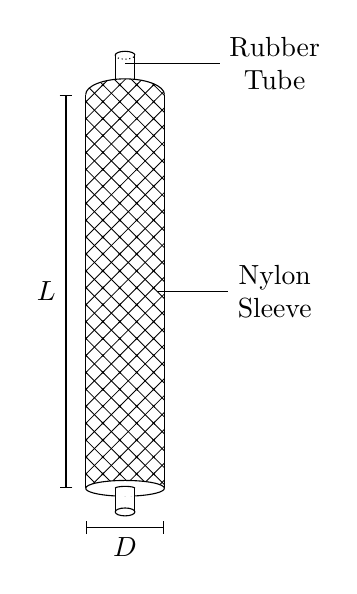
\begin{tikzpicture}
			\draw (0,0) arc (0:180:0.5 and 0.2);
			\draw (-1,0) -- (-1,-5);
			\draw (0,-5) -- (0,0);
			\draw[] (-0.625,0.2) -- (-0.625,0.5);
			\draw[] (-0.375,0.5) arc(0:180:0.125 and 0.05);
			\draw[densely dotted] (-0.625,0.5) arc(180:360:0.125 and 0.05);
			\draw[] (-0.375,0.5) -- (-0.375,0.2);
			\pattern[pattern=north east hatch,hatch distance=2.5mm] (-1,0) -- (-1,-5) arc(180:360:0.5 and 0.1) -- (0,0) arc (0:180:0.5 and 0.2);
			\pattern[pattern=north west hatch,hatch distance=2.5mm] (-1,0) -- (-1,-5) arc(180:360:0.5 and 0.1) -- (0,0) arc (0:180:0.5 and 0.2);
			\fill[white] (0,-5) arc(0:360:0.5 and 0.1);
			\draw (-1,-5) arc(180:255:0.5 and 0.1);
			\draw (0,-5) arc(360:285:0.5 and 0.1);
			\draw (0,-5) arc(0:180:0.5 and 0.1);
			\draw[] (-0.375,-5) arc(0:180:0.125 and 0.025);
			\draw[] (-0.625,-5) -- (-0.625,-5.3);
			\draw[] (-0.625,-5.3) arc(180:360:0.125 and 0.05);
			\draw[] (-0.375,-5.3) arc(0:180:0.125 and 0.05);
			\draw[] (-0.375,-5.3) -- (-0.375,-5);
			\node at (-1.25,0) (nA) {};
			\node at (-1.25,-5) (nB) {};
			\node[align=center] at (1.4,0.4) (tubeText) {Rubber \\ Tube};
			\node[align=center] at (1.4,-2.5) (sleeveText) {Nylon \\ Sleeve};
			\draw (-0.5,0.4) -- (tubeText);
			\draw (-0.1,-2.5) -- (sleeveText);
			\Dimline[($(nB)$)][($(nA)$)][$L$][0.25];
			\node at (-1,-5.5) (nC) {};
			\node at (0,-5.5) (nD) {};
			\Dimline[($(nC)$)][($(nD)$)][$D$][-0.25];
		\end{tikzpicture}
	\end{minipage}
	\begin{minipage}{.4\textwidth}
		\centering
		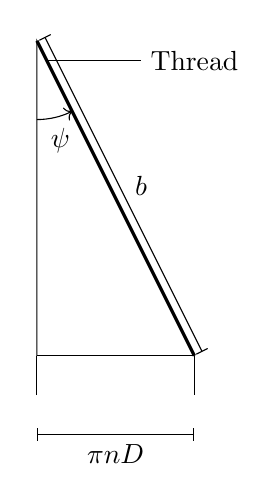
\begin{tikzpicture}
			\draw (0,0) coordinate (L) node {}
				-- (0,4) coordinate (O) node {}
				-- (2,0) coordinate (R) node {}
				pic["$\psi$", ->,draw=black, angle eccentricity=1.3, angle radius=1cm]{angle=L--O--R};
			\draw (0,-0.5) -- (0,0);
			\draw (0,0) -- (2,0);
%			\filldraw[] (0,4) circle (1pt);
			\draw[very thick] (0,4) -- (2,0);
			\draw (2,0) -- (2,-0.5);
			\node at (2,3.75) (threadText) {Thread};
			\draw (0.11,3.75) -- (threadText);
			\node at (0,-1) (nA) {};
			\node at (2,-1) (nB) {};
			\Dimline[($(nA)$)][($(nB)$)][$\pi n D$][-0.25];
			\node at (0.1,4.05) (nO) {};
			\node at (2.1,0.05) (nC) {};
			\Dimline[($(nO)$)][($(nC)$)][$b$][0.25];
		\end{tikzpicture}
	\end{minipage}
	\caption{Geometric structure of a McKibben artificial muscle}
	\label{fig:muscle_structure}
\end{figure}

\begin{align}
	L = b\cos(\psi),\quad D = \frac{b \sin(\psi)}{n \pi} 
	\label{eq:geom_rel_1}
\end{align}
where $L$ is the length of the muscle, $D$ is the outer diameter of the muscle,
$b$ is the thread length, $n$ is the number of turns of a thread,
and $\psi$ is the angle formed by the sleeve's threads and its vertical axis.

\subsection{Static Model of the Muscle}

The input work $W_{in}$ is applied to the muscle when the fluid (liquid or air)
pushes the internal surface of the rubber tube.
This can be expressed as the product of the supply pressure and the change in volume.

\begin{align}
	dW_{in} = \left( P - P_0 \right)dV = P'dV
	\label{eq:input_work}
\end{align}

Where $P$ is the supply pressure, $P_0$ is the atmospheric pressure,
$P'$ is the pressure difference and $dV$ is the volumetric change.

Equation~\ref{eq:muscle_volume} shows the volume of the muscle,
with the assumption that it has cylindrical shape.

\begin{align}
	V = \frac{1}{4}\pi L D^2
	\label{eq:muscle_volume}
\end{align}

Then, from Equation~\ref{eq:geom_rel_1},

\begin{align}
	V = \frac{1}{4}\pi L D^2 = \frac{b^3}{4 \pi n^2}\sin(\psi)^2\cos(\psi)
	\label{eq:volume_psi}
\end{align}

When the actuator contracts, the output work of the system $W_{out}$ is given by
Equation~\ref{eq:output_work}.

\begin{align}
dW_{out} = F \times (-dL) \label{eq:output_work}
\end{align}

Where $F$ is the axial tension, and $dL$ is the axial displacement change.

From Equation~\ref{eq:geom_rel_1} we can express $\nicefrac{dL}{d \psi}$ as follows.

\begin{align}
\frac{dL}{d \psi} = -b \sin{(\psi)} \label{eq:L_derivative}
\end{align}
With the assumption that the input work and the output work should be equal
if the system is lossless and without energy storage, as for
Equations~\ref{eq:input_work},~\ref{eq:volume_psi},~\ref{eq:output_work} and~\ref{eq:L_derivative},
then the relation shown in Equation~\ref{eq:F_final} can be obtained.

\begin{align}
F = -P'\frac{\nicefrac{dV}{d \psi}}{\nicefrac{dL}{d \psi}} = \frac{\pi P'}{4}\left(\frac{b}{\pi n}\right)^2 \left(3 \cos^2(\psi) - 1 \right)\label{eq:F_final}
\end{align}

From this, it can be observed that the tension $F$ is linearly proportional to the
pressure difference $P'$, and it is a monotonic function of the angle $\psi$ $(0\degree < \psi < 90\degree)$.

\subsection{Modified Static Model}

The static model of a McKibben muscle can be expressed as Equation~\ref{eq:F_final}.
However, that model does not take into account the thickness $t_k$ of both the nylon
sleeve and the internal rubber tube. If this is considered, then the volume calculated
in Equation~\ref{eq:muscle_volume} becomes the following.

\begin{align}
V &= \frac{1}{4}\pi L \left(D - 2 t_k \right)^2 \nonumber \\
&= \frac{b^3}{4 \pi n^2}\sin{(\psi)}\left(3 \cos^2(\psi) - 1 \right)-b \cos{(\psi)}t_k
\left(\frac{b}{n}\sin{(\psi)}-\pi t_k\right) \label{eq:muscle_volume_thickness}
\end{align}

From Equation~\ref{eq:muscle_volume_thickness} then it is possible to obtain
the equivalent of Equation~\ref{eq:F_final} with thickness included.
The result is shown in Equation~\ref{eq:F_final_thickness}.

\begin{align}
	F = \frac{b^2 P'}{4 \pi n^2}\left(3 \cos^2{(\psi)} \right)+\pi t_k P' 
	\left [\frac{b}{\pi n}\left( 2 \sin (\psi) - \frac{1}{\sin (\psi)} \right) - t_k \right]
	\label{eq:F_final_thickness}
\end{align}

\subsection{Static Model Validation}

% TODO: Describe the system used for testing and identification

It is possible to validate the static model obtained. Stepwise voltage is applied
to the input and output proportional valves, to study the behaviour of the muscle
under quasi static conditions.

{\color{red}(Aggiungere validazione del modello con enfasi sull'errore derivante attriti e approssimazioni)}

\clearpage

\section{Muscle Model Based on System Identification}

If all sources of non linearity could be taken into account,
then theoretical models may agree with experimental results.
However, by taking into consideration these elements, the models would become
very complex and they would be difficult to control. 
Moreover, the models would lack in versatility, meaning that these parameters
would have to be changed for different muscles and weights.

The model of the muscle is thus obtained through
linear system identification techniques and tools such as MATLAB and Simulink.
In this section the derivation of the muscle model based on system identification
is described, as well as the improvement of the identified model
by using the Bouc-Wen model of hysteresis.

% TODO: Consider if it is necessary to add the pre-identification step
% TODO: Aggiungere almeno i dettagli riguardo il rising time del muscolo e il peso utilizzato

\subsection{Identification Experiments}
\label{sec:4.ide}

For the identification step, a stepwise signal has been generated
and given to the input and output proportional valves. The two signals are symmetric
one another, due to the nature of the valves. They range from 0 to 10 Volts,
and are shown in figure~\ref{fig:input_voltage}. The algorithm for generating the signals
is in Appendix~\ref{app:algorithms} (Algorithm~\ref{alg:step_input_generation}).

% TODO: immagine sbagliata, devono essere secondi alla -1
\begin{figure}[h]
	\centering
	\includegraphics[width=\linewidth]{"Images/stair_input_waves"}
	\caption[Input waves for proportional valves]{Input waves for proportional valves}
	\label{fig:input_voltage}
\end{figure}

Figure~\ref{fig:disp_press} shows the pressure and displacement characteristics
of the muscle with the input just introduced.

\begin{figure}[H]
	\centering
	\includegraphics[width=\linewidth]{"Images/pressure_displacement"}
	\caption[Pressure and displacement characteristic]{Pressure and displacement characteristic}
	\label{fig:disp_press}
\end{figure}

By plotting this data with pressure on the x-axis and displacement on the y-axis,
it is possible to notice the hysteretic behaviour of the muscle,
as shown in Figure~\ref{fig:hysteresis_plot}.

\begin{figure}[H]
	\centering
	\includegraphics[width=\linewidth]{"Images/hysteresis_plot"}
	\caption[Pressure and displacement characteristic]{Pressure and displacement characteristic - Hysteresis plot}
	\label{fig:hysteresis_plot}
\end{figure}

Using the MATLAB System Identification Toolbox~\cite{ide_toolbox},
we can get a discrete transfer function from input and output values.
The description on how to use the toolbox is provided in Appendix~\ref{app:toolbox}.

The input and output data are given to the toolbox. 
After that, input and output data are treated in the following way:
\begin{itemize}
	\item their mean is put to 0
	\item the data is split in half and used in the following way:
	\begin{itemize}
		\item the first half is used for the \textit{estimation process},
		by which the toolbox attempts to find a discrete function
		that correctly approximates the input-output characteristic of the system.
		\item the second half is used for the \textit{validation process},
		by means of which the toolbox computes the fit of the identified transfer function.
	\end{itemize}
\end{itemize}  

The toolbox permits to select the number of zeros and poles that the transfer function
must present. A number of 1 poles and 1 zeros has been chosen for this step.

The identification step then provides the discrete transfer function
in Equation~\ref{eq:disc_tf}, where L(z) and P(z) represent respectively the z transform
of displacement and pressure.

\begin{align}
G(z) = \dfrac{L(z)}{P(z)} = \dfrac{24.9366\ z^{-1}}{1-0.9618\ z^{-1}}
\label{eq:disc_tf}
\end{align}

{\color{red}Se necessario, è possibile usare una funzione di trasferimento con due poli e due zeri invece di una con un polo ed uno zero}

The fit of this transfer function with respect to experimental data is shown
in Figure~\ref{fig:fit}.

\begin{figure}[H]
	\centering
	\includegraphics[width=\linewidth]{"Images/fit"}
	\caption[Transfer function fit]{Transfer function fit}
	\label{fig:fit}
\end{figure}

It is possible to raise the number of poles and zeros of the transfer function
in order to improve its fit with respect to experimental data. 
The trade-off is that the resulting transfer function will be more complex.

{\color{red}Aggiungere diagramma pressione-displacement sperimentale e il corrispettivo diagramma derivante dalla funzione di trasferimento identificata}

The transfer function in Equation~\ref{eq:disc_tf} can be written rewritten as follows

\begin{align}
L(z) - 0.9618 L(z)z^{-1}  = 24.9366 P(z) z^{-1}
\label{eq:l_k_1}
\end{align}

This implies

\begin{align}
l(k) &= 0.9618 l(k-1) + 24.9366p(k-1) \nonumber \\
&= a l(k-1) + b p(k-1) \label{eq:l_k_2}\\
&a = 0.9618, \quad b = 24.9366 \nonumber
\end{align}

So the displacement at step k depends on the displacement and pressure
at the previous step.

\section{Hysteresis Modeling}

Hysteresis represents a property of systems that show
the dependence of their state from their history.
It is a nonlinear phenomenon exhibited by systems stemming
from various science and engineering areas: under a low-frequency
periodic excitation, the relationship between the system’s input and
output is not the same for loading and unloading
This means that the same input applied at different times can yield
different output with respect to the history of the system.

The etymology of the term "hysteresis" is derived from the ancient Greek,
and it means "delay" or "lagging behind".

A fundamental theory that allows a general framework
for modeling hysteresis has not been developed yet.

For specific problems, models derived from a general understand of physics
are normally used. This kind of models are, however, hard to derive and
difficult to use in practical application due to their complexity.
For this reason, alternative models of these complex systems have been proposed.
Phenomenological (or semi-physical) models are simpler models that,
although not giving the best description of the behaviour of a system,
combine some physical understanding of the system along with
some kind of black-box modeling, keeping relevant
input-output information that is useful for characterization,
design and control purposes.

{\color{red}Aggiungere descrizione dettagliata isteresi e introdurre cosa si leggerà in seguito}

\section{Models of Hysteresis}

There is a large variety of hysteresis models available in literature,
such as:

\begin{itemize}[noitemsep]
	\item the Preisach model~\cite{preisach}, used to model electromagnetic hysteresis
	\item the Maxwell-Slip model~\cite{maxwell-slip}, used for friction simulation and compensation,
	\item the Bouc-Wen model, extensively used in the areas of smart structures
	and civil engineering~\cite{bouc_wen}
\end{itemize}

The latter consists of a first-order nonlinear differential equation that relates
the input displacement to the output restoring force
in a rate-independent hysteretic way~\cite{krasnosel2012systems}.

\section{The Bouc-Wen Model of Hysteresis}

Proposed by Bouc~\cite{bouc} in 1971 and later modified by Wen~\cite{bouc_wen} in 1976,
the Bouc-Wen model has been vastly used to mathematically describe components and devices
that present hysteretic behaviours, particularly within
the areas of civil and mechanical engineering.

The differential equation consists of several parameters. By choosing them appropriately,
it is possible to accommodate the response of the model to the real hysteresis
loop~\cite{ismail2009hysteresis}.
The derivation of the model is available in Appendix~\ref{app:bouc-wen}.

Equation~\ref{eq:l_k_2} can be modified by adding a virtual hysteresis component.
This should allow the hysteresis loop to adapt to the experimental values by changing
the model's parameters.

\begin{align}
\label{eq:l_w}
l(k) &= a \left [\alpha l(k-1) + (1-\alpha)w(k-1) \right] + bp(k-1) \\
\alpha &\in \left[0,1\right],\quad a = 0.9618, \quad b=24.9366 \nonumber
\end{align}
Here $w$ is a virtual hysteresis variable introduced by the use of Bouc-Wen model.
It is possible to implement two different versions of the hysteresis model:
\begin{itemize}[noitemsep]
	\item the one proposed by Bouc and modified by Wen, that will be henceforth called \textit{classic} version
	\item a more recent and flexible version proposed by Song and Der Kiureghian, that will be called \textit{generalized} version
\end{itemize}

\subsection{Classic Bouc-Wen Hysteresis Model}
The classic Bouc-Wen model's virtual hysteresis variable $w$ is described by Equation~\ref{eq:w_classic_continuous}.

\begin{align}
\dot{w} = A\dot{l} - \beta \abs{\dot{l}} \abs{w}^{n-1} - \gamma \dot{l} \abs{w}^n
\label{eq:w_classic_continuous}
\end{align}

$A$, $\beta$, $\gamma$ and $n$ are Bouc-Wen model's parameters.
They control the shape and the slope of the hysteretic loop.
Further details are described in Appendix~\ref{app:bouc-wen}.

\subsection{Generalized Bouc-Wen Hysteresis Model}
Song and Der Kiureghian~\cite{song2006generalized} proposed a generalized Bouc-Wen model for highly asymmetric
hysteresis that in certain cases shown higher flexibility
and resiliency than the classic Bouc-Wen model.

The generalized Bouc-Wen model's virtual hysteresis variable $w$
is described by Equations~\ref{eq:bw_generalized} and ~\ref{eq:bw_psi}.


\begin{align}
\dot{w} &= \dot{l} \left[A - \abs{w} \Psi(l, \dot{l}, w)\right] \label{eq:bw_generalized}\\
\Psi(l, \dot{l}, w) &= \beta_1 \sign(\dot{l}w) + \beta_2 \sign(l\dot{l}) + \beta_3 \sign(lw) \nonumber \\
&+ \beta_4 \sign(\dot{l}) + \beta_5 \sign(w) + \beta_5 \sign(l) \label{eq:bw_psi}
\end{align}
where $\beta_1,\ldots,\beta_6$ are fixed parameters.
\section{Hysteresis Variable Approximation}
Equations~\ref{eq:w_classic_continuous} and~\ref{eq:bw_generalized} should be approximated to a discrete time equation, as Equation~\ref{eq:l_w} is in discrete time. To do so, it is possible to use forward
difference approximation method, as shown in Equations~\ref{eq:approx_1} and~\ref{eq:approx_2}. $T_s$ represents the sampling time for the approximation.

\begin{align}
\frac{dx}{dt} &\approx \frac{x(t+T_s) - x(t)}{T_s} = \frac{x(k+1) - x(k)}{T_s} \label{eq:approx_1}\\
\frac{d^2x}{dt^2} &\approx \frac{x(t+2T_s) - 2x(t+T_s) + x(t)}{T_s^{2}} =
\frac{x(k+2)-2x(k+1)+x(k)}{T_s^2} \label{eq:approx_2}
\end{align}
\subsection{Classic Bouc-Wen Model}

In the classic version of the Bouc-Wen model,
the virtual hysteresis variable $w$ can be discretized as follows.

\begin{align}
\frac{w(k+1)-w(k)}{T_s} &= A \frac{l(k+1)-l(k)}{T_s} - \beta \abs{\frac{l(k+1)-l(k)}{T_s}}\abs{w(k)}^{n-1} \nonumber \\ 
&- \gamma \frac{l(k+1)-l(k)}{T_s} \abs{w(k)}^n
\end{align}

Solving for $w(k)$ gives the result in Equation~\ref{eq:w(k)}.

\begin{align}
w(k) &= A\left[l(k)-l(k-1)\right] - \beta \abs{l(k)-l(k-1)}\abs{w(k-1)}^{n-1} \nonumber \\
 &- \gamma \left[l(k)-l(k-1)\right]\abs{w(k-1)}^n + w(k-1)
 \label{eq:w(k)}
\end{align}

\subsection{Generalized Bouc-Wen Model}

In the generalized version of the Bouc-Wen model,
the virtual hysteresis variable $w$ can be discretized as follows.
\begin{align}
\frac{w(k+1)-w(k)}{T_s} = \frac{l(k+1)-l(k)}{T_s}\left[A - \abs{w(k)}\Psi(l,w,k)\right]
\label{eq:w_generalized_cont}
\end{align}
\begin{equation}
	\begin{split}
	\Psi(l,w,k)&=\beta_1\sign\left(\left[\frac{l(k+1)-l(k)}{T_s}\right]w(k)\right) \\
	&+\beta_2 \sign\left(\left[\frac{l(k+1)-l(k)}{T_s}\right]l(k)\right) \\
	&+\beta_3 \sign\left(l(k)w(k)\right) + \beta_4 \sign\left(\frac{l(k+1)-l(k)}{T_s}\right) \\
	&+\beta_5 \sign\left(w(k)\right) + \beta_6 \sign\left(l(k)\right)
	\end{split}
\end{equation}

Solving Equation~\ref{eq:w_generalized_cont} for w(k) gives the result in Equation~\ref{eq:w_generalized}.

\begin{equation}
\begin{split}
w(k) &= \left[l(k)-l(k-1)\right]\left[A-\abs{w(k)}\Psi(l,w,k)\right]+w(k-1) \\
\Psi(l,w,k) &= \beta_1\sign\left(\left[l(k)-l(k-1)\right]w(k)\right) \\
&+\beta_2\sign\left(\left[l(k)-l(k-1)\right]l(k)\right) \\
&+\beta_3\sign\left(l(k)w(k)\right) + \beta_4\sign\left(l(k)-l(k-1)\right) \\
&+\beta_5 \sign\left(w(k)\right) + \beta_6 \sign\left(l(k)\right)
\end{split}
\label{eq:w_generalized}
\end{equation}

\section{Identified Model Summation}

The previous sections can be summarized with Equations~\ref{eq:final_class} and~\ref{eq:final_gen}.

\subsection{Classic Bouc-Wen Model}

\begin{equation}
	\begin{cases}
		l(k) = a \left [\alpha l(k-1) + (1-\alpha)w(k-1) \right] + bp(k-1) \\
		w(k) = A\left[l(k)-l(k-1)\right] - \beta \abs{l(k)-l(k-1)}\abs{w(k-1)}^{n-1} \\
		\qquad \quad- \gamma \left[l(k)-l(k-1)\right]\abs{w(k-1)}^n + w(k-1) \\
		\qquad \quad \alpha \in \left[0,1\right],\quad a = 0.9618, \quad b=24.9366
	\end{cases}
	\label{eq:final_class}
\end{equation}

\subsection{Generalized Bouc-Wen Model}

\begin{equation}
	\begin{cases}
		l(k) = a \left [\alpha l(k-1) + (1-\alpha)w(k-1) \right] + bp(k-1) \\
		w(k) = \left[l(k)-l(k-1)\right]\left[A-\abs{w(k)}\Psi(l,w,k)\right]+w(k-1) \\
		\Psi(l,w,k) = \beta_1\sign\left(\left[l(k)-l(k-1)\right]w(k)\right) \\
		\qquad \qquad \quad+\beta_2\sign\left(\left[l(k)-l(k-1)\right]l(k)\right) \\
		\qquad \qquad \quad+\beta_3\sign\left(l(k)w(k)\right) + \beta_4\sign\left(l(k)-l(k-1)\right) \\
		\qquad \qquad \quad+\beta_5 \sign\left(w(k)\right) + \beta_6 \sign\left(l(k)\right) \\
		\qquad \qquad \quad \alpha \in \left[0,1\right],\quad a = 0.9618, \quad b=24.9366
	\end{cases}
	\label{eq:final_gen}
\end{equation}

\section{Evaluation of Proposed Models}
\label{sec:4.eva}

The models previously proposed are tested and evaluated to estimate
the error with respect to experimental data. 

Without taking the Bouc-Wen model into consideration, 
given experimental input values $p$, using equation~\ref{eq:disc_tf}
the simulated output $\hat{l}$ with respect the experimental values $l$
is shown in Figure~\ref{fig:comparison}.

\begin{figure}[H]
	\centering
	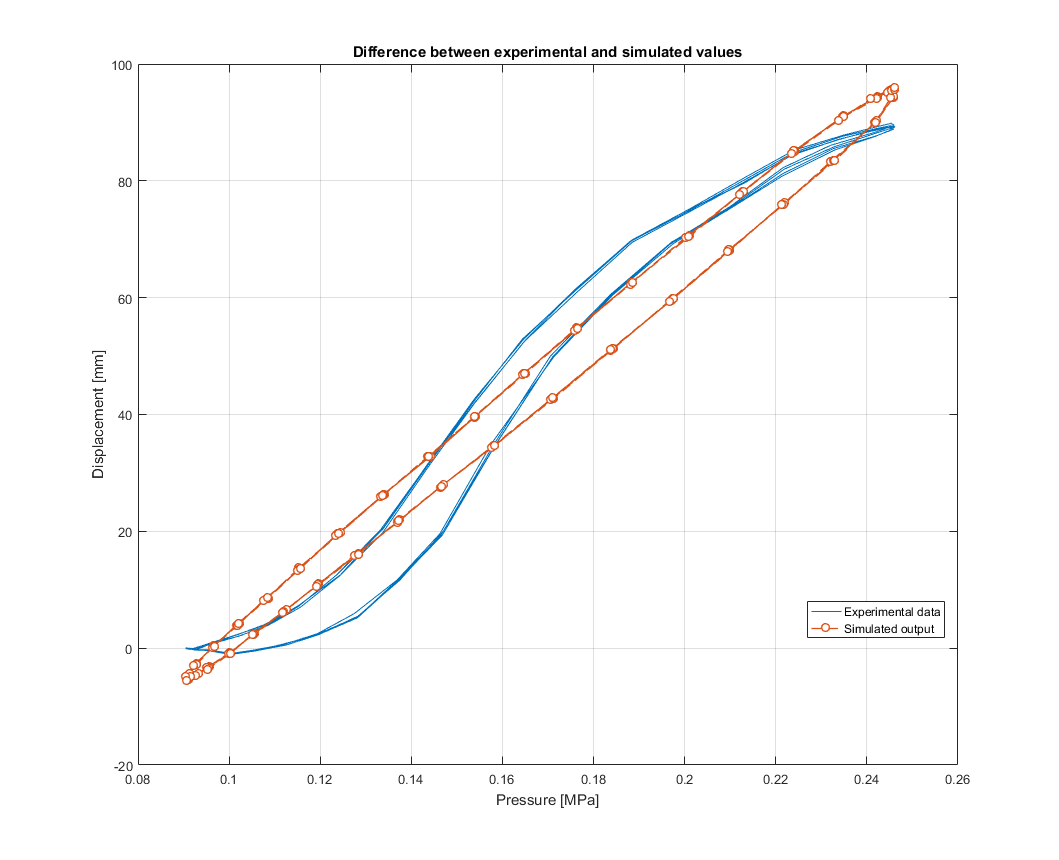
\includegraphics[width=\linewidth]{Images/comparison}
	\caption[Comparison between experimental data and simulated output]{Comparison between experimental data and simulated output}
	\label{fig:comparison}
\end{figure}

If the Bouc-Wen model is taken into consideration, then the parameters
must be fixed appropriately. To get a fairly good fit it is possible to tune
these parameters by trial and error. Further methods for finding the best sets
of parameters for the hysteresis model are discussed in Chapter~\ref{ch:optimization}.

\subsection{Classic Bouc-Wen Model Parameters}

\begin{minipage}{0.6\textwidth}
	\vspace*{-0.25cm}
	The parameters to be chosen for the classic version of the Bouc-Wen model are
	$\alpha$, $A$, $\beta$, $\gamma$ and $n$. For this work, $n$ will be fixed at 1
	for both the classic and generalized version of the hysteresis model.
	Details about how each parameters alters the shape of the hysteretic loop
	are in Appendix~\ref{app:bouc-wen}. 
	
	The parameters in Table~\ref{tab:classic_param} have been fixed by trial and error.
	All parameters are adimensional.	
\end{minipage}
\hfill
\begin{minipage}{0.35\textwidth}
	\vspace*{-0.5cm}
	\begin{table}[H]
		\centering
		\begin{tabular}{@{}cl@{}}
			\toprule
			\textbf{Parameter} & \textbf{Value} \\ \midrule
			$\alpha$           & $0.5$          \\
			$A$                & $0.9$          \\
			$\beta$            & $0.002$        \\
			$\gamma$           & $-0.001$       \\
			$n$                & $1$            \\ \bottomrule
		\end{tabular}
		\caption{Parameters for the Classic Bouc-Wen Model}
		\label{tab:classic_param}
	\end{table}
\end{minipage}

\vspace*{0.5cm}

Given experimental input $p$, the simulated output of the system taking into consideration
the classic Bouc-Wen model of hysteresis is shown in Figure~\ref{fig:comp_classic}.

\begin{figure}[H]
	\centering
	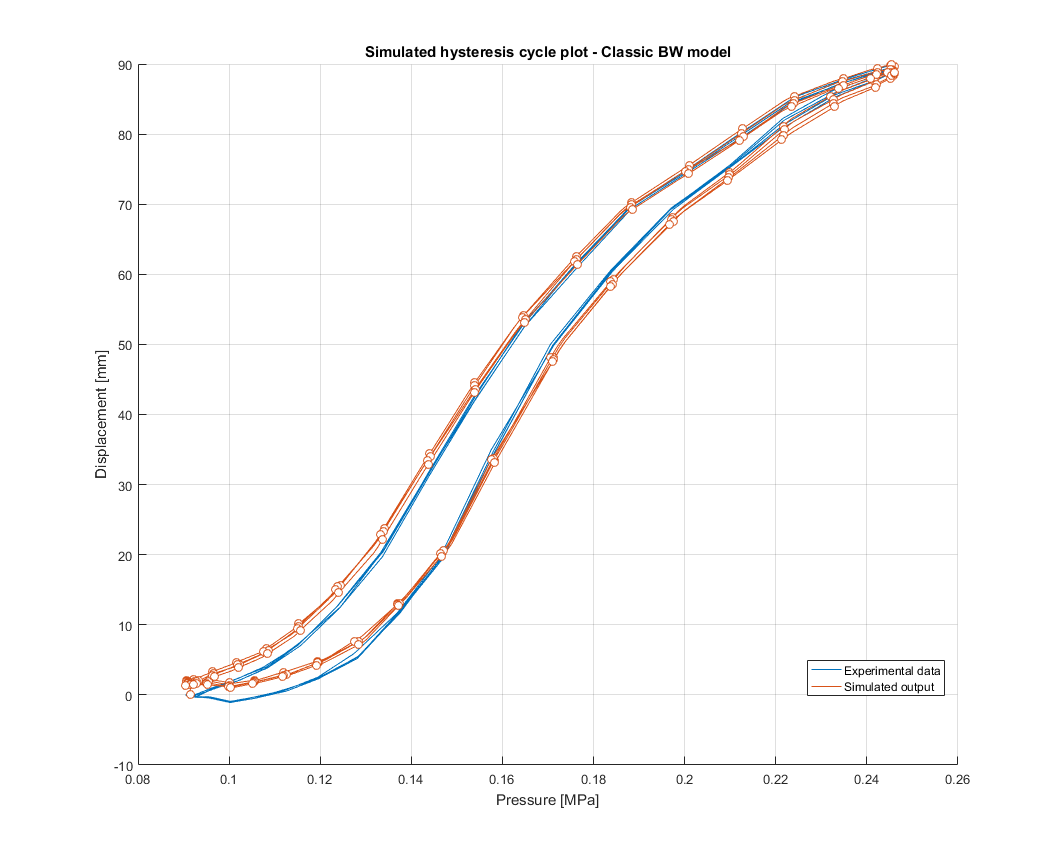
\includegraphics[width=\linewidth]{Images/comparison_classic}
	\caption[Comparison between experimental data and simulated output with classic Bouc-Wen model]{Comparison between experimental data and simulated output with classic Bouc-Wen model}
	\label{fig:comp_classic}
\end{figure}

\subsection{Generalized Bouc-Wen Model Parameters}

\begin{minipage}[ht]{0.6\textwidth}
	\vspace*{-2cm}
	The parameters to be chosen for the generalized version of the Bouc-Wen model
	are $\alpha$, $A$, $n$, $\beta_1$, \ldots, $\beta_6$. 
	As previously stated, the value of $n$ is fixed to $1$.
	
	As for the classic version of the hysteresis model, the parameters
	in Table~\ref{tab:gener_param} have been selected by trial and error.
	All parameters are adimensional.
	
	Given experimental input $p$, the simulated output of the system
	after taking into consideration the generalized Bouc-Wen model of hysteresis
	is shown in Figure~\ref{fig:comp_gener}.
\end{minipage}
\hfill
\begin{minipage}{0.35\textwidth}
	\vspace*{-0.5cm}
	\begin{table}[H]
		\centering
		\begin{tabular}{@{}cl@{}}
			\toprule
			\textbf{Parameter} & \textbf{Value} \\ \midrule
			$\alpha$           & $0.9$          \\
			$A$                & $1$          	\\
			$n$   		       & $1$        	\\
			$\beta_1$          & $0.01$       	\\
			$\beta_2$          & $0.005$       	\\
			$\beta_3$          & $0.1$       	\\
			$\beta_4$          & $-0.01$       	\\
			$\beta_5$          & $-0.1$       	\\
			$\beta_6$          & $0.001$       	\\ \bottomrule
		\end{tabular}
		\caption{Parameters for the Generalized Bouc-Wen Model}
		\label{tab:gener_param}
	\end{table}
\end{minipage}

\begin{figure}[H]
	\centering
	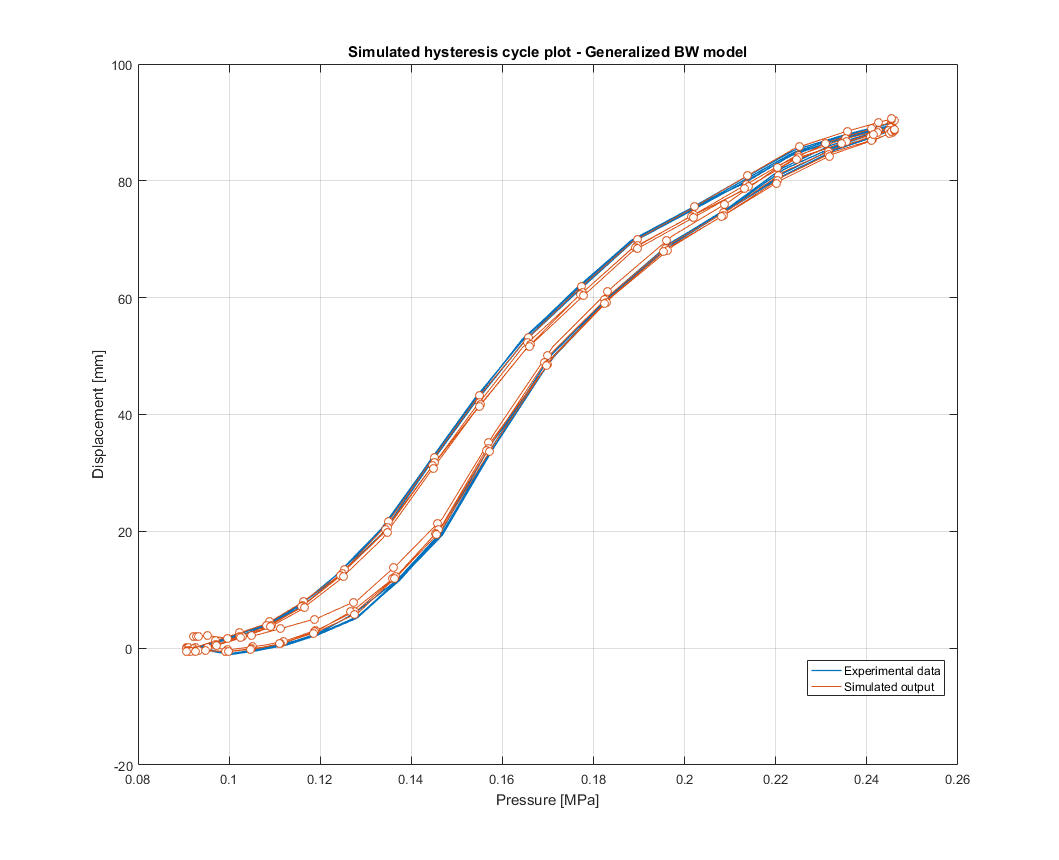
\includegraphics[width=\linewidth]{Images/comparison_general}
	\caption{Comparison between experimental data and simulated output with generalized Bouc-Wen model}
	\label{fig:comp_gener}
\end{figure}
 % Chapter 4 - Model
% PID - MPC Controller design and comparison

\chapter{Controller Design}
\label{Chapter5} 























 % Chapter 5 - Parameter Optimization: GA, Firefly, PSO
% PID - MPC Controller design and comparison

\chapter{Controller Design}
\label{ch:control} 

\section{Introduction}
\label{sec:6.intro}

To achieve precise position control, a PI controller has been developed,
simulated and then tested onto real equipment. The controller has been tested
using a sine wave reference with different frequencies for each run,
from 1 to 3 $\nicefrac{rad}{s}$.

The weight lifted by the muscle is also variable,
and experiments have been done with weights of 4.5 kg and 7 kg.
To connect the MATLAB suite and the real apparatus,
a Simulink model has been developed. The connection is achieved
by using a dSPACE~\cite{dspace} DS1104 Controller Board,
which upgrades a PC to a development system for rapid control prototyping,
and that can be seen in Figure~\ref{fig:dspace}.
The Controller Board can be installed in any PCI or PCIe slot.

The Controller Board has been connected to several components,
to monitor important model variables (i.e. the muscle's pressure)
and apply control input to two proportional valves.

\begin{figure}[H]
	\centering
	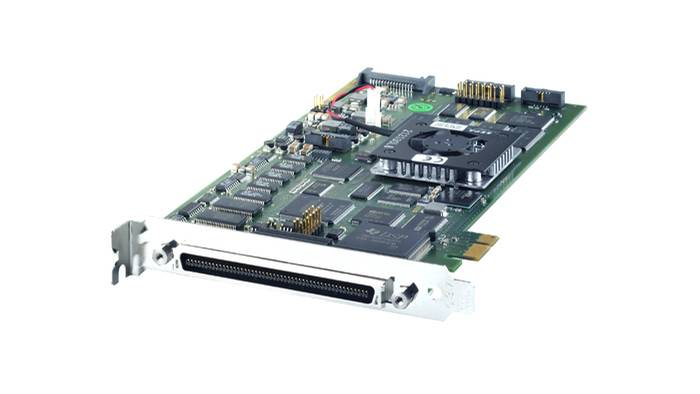
\includegraphics[width=\linewidth]{Images/dspace}
	\caption{DS1104 R\&D Controller Board}
	\label{fig:dspace}
\end{figure}

\section{PI Controller Development}

\subsection{Introduction on PID Control}

Figure~\ref{fig:pid} shows a block diagram of a PID controller in a feedback loop.
The idea behind PID control is to keep track of the error and trying to minimize it,
using three control terms of proportional, integral and derivative.
The action of these three control terms influence the controller output
in order to apply accurate and optimal control.

\tikzstyle{int}=[draw, fill=Maroon!20, minimum size=2em, text width=2.2cm]
\tikzstyle{sum}=[draw, fill=Maroon!20, shape=circle, node distance=2.5cm]
\begin{figure}[H]
	\centering
	\begin{tikzpicture}[node distance=1.5cm,auto,>=latex]
	\node [int] (kp) {P $K_p e(t)$};
	\node [int] (ki) [below of=kp] {I $K_i \int{e(t)dt}$};
	\node [int] (kd) [below of=ki] {D $K_d \frac{e(t)}{dt}$};
	\node [sum] (sum) [right of=ki] {$\sum$};
	\node [sum] (sub) [left of=ki, node distance=3.25cm] {$\sum$};
	\node [coordinate] (joint1) [left of=ki, node distance=2cm]{};
	\node [coordinate] (begin) [left of=sub, node distance=2cm]{};
	\node [int] (plant) [right of=sum, node distance=3cm] {Plant};
	\node [coordinate] (end) [right of=plant, node distance=3cm]{};
	\draw[-] (begin) -- node {$r(t)$} (sub);
	\draw[-] (begin) -- node [pos=0.9] {$+$} (sub.west);
	\draw[-] (sub) -- node [pos=0.2] {$e(t)$} (ki);
	\draw[->] (joint1) |- (kp.west);
	\draw[->] (joint1) -- (ki);
	\draw[->] (joint1) |- (kd);
	\draw[->] (kp.east) -| node [pos=0.95] {$+$} (sum.north);
	\draw[->] (ki.east) -- node [pos=0.8] {$+$} (sum.west);
	\draw[->] (kd.east) -| node [pos=0.95] {$+$} (sum.south);
	\draw[->] (sum.east) -- node {$u(t)$} (plant);
	\draw[->] (plant.east) -- node {$y(t)$} (end);
	\draw[->] ($(end.west)!0.5!(plant.east)$) -- ($(end.west)!0.5!(plant.east)+(0,-2.5)$) -| node [pos=0.95] {$-$} (sub.south) {};
	\end{tikzpicture}
	\caption{Block diagram of a PID controller in a feedback loop}
	\label{fig:pid}
\end{figure}

Given the error $e(t)$ as the difference between the reference $r(t)$
and the output $y(t)$, the three components act as follows:

\begin{itemize}
	\item The term P is proportional to the current value of $e(t)$.
	\item The term I takes into account past values of $e(t)$. 
		The integral term seeks to eliminate the residual error by adding
		a control effect due to the historic cumulative value of the error.
	\item The term D is a best estimate of the future trend of $e(t)$.
	The more rapid the error changes, the greater will be
	the controlling or dampening effect
\end{itemize}

The overall control function can be expressed mathematically as in Equation~\ref{eq:pid}.

\begin{align}
\label{eq:pid}
u(t) = K_p e(t) + K_i \int_0^t{e(t)dt} + K_d \frac{de(t)}{dt}
\end{align}

The PID control is easy to develop and to apply. 
The main drawback is the tuning of the control gains $K_i$, $K_i$ and $K_p$
depending on the features of the system. For example, in the case of McKibben
muscles it may be necessary to tune the control when the load is changed
or for different kinds of muscles.

The use of the PID algorithm does not guarantee optimal control of the system
nor its control stability. Moreover situations may arise where there are excessive delays:
the measurement of the process value is delayed,
or the control action does not apply quickly enough to guarantee stability.

\subsection{Application of PI Control}

As introduced in Section~\ref{sec:6.intro}, the control has been applied onto
a real McKibben muscle in a laboratory environment. 
The reference $r(t)$ has been set as a sine wave, with variable frequency of 1, 2 and 3
$\nicefrac{rad}{s}$.

Section~\ref{sec:6.4.5kg} covers the application of PI control on the laboratory
muscle with a weight of 4.5 kilograms, and Section~\ref{sec:6.7kg} concerns
the application of PI control with a weight of 7 kilograms.

The hysteresis model used for control is the classic Bouc-Wen model.
The model parameters used are obtained offline beforehand using the Modified Firefly
Algorithm, described in Section~\ref{sec:5.mfa}.

The reference signal $r(t)$ has an amplitude of 10 millimetres, a bias of 30
and variable frequency. The code to generate this kind of wave
is in Appendix~\ref{app:algorithms}.

\subsubsection{Application on Muscle -- 4.5 Kilograms Weight}
\label{sec:6.4.5kg}

This Section covers the application of PI control on a real McKibben artificial muscle
driven by tap-water. The weight attached to the muscle weighs 4.5 kilograms.

The PID gains have been set as those of Table~\ref{tab:pid_gains_45}
for all three frequencies, to show the limitations of this kind of control.

\begin{table}[H]
	\centering
	\begin{tabular}{l c c c}
		\toprule
		\textbf{Gain parameter}	& $K_p$		& $K_i$		& $K_d$ \\ \midrule
		\textbf{Value}			& $0.06875$	& $0.05$	& $0$ \\ \bottomrule
	\end{tabular}
	\caption{PID gains}
	\label{tab:pid_gains_45}
\end{table}

\begin{figure}[H]
	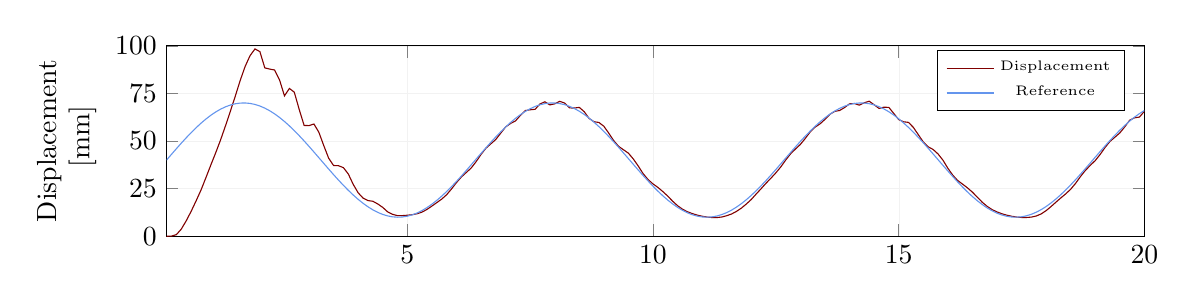
\begin{tikzpicture}
	\begin{axis}[
	ylabel style={align=center},
	ylabel={Displacement\\~[mm]},
	xmin=1, xmax=200,
	ymin=0, ymax=100,
	legend style={font=\tiny},
	grid=both,
	grid style={line width=.1pt, draw=gray!10},
	width=14cm,height=4cm,
	xticklabels={0,5,10,15,20},xtick={0,50,100,150,200},
	ytick={0,25,50,75,100},
	%thick
	]
	
	\addplot[
	color=Maroon
	]
	coordinates {
(1,0)(2,0.0700000000000000)(3,0.840000000000000)(4,3.73000000000000)(5,8.07000000000000)(6,13.0400000000000)(7,18.4800000000000)(8,24.1600000000000)(9,30.6700000000000)(10,37.3000000000000)(11,43.7900000000000)(12,50.6000000000000)(13,58.0100000000000)(14,65.7400000000000)(15,73.6200000000000)(16,81.8800000000000)(17,89.1900000000000)(18,94.8500000000000)(19,98.3600000000000)(20,96.9500000000000)(21,88.4000000000000)(22,87.7900000000000)(23,87.2800000000000)(24,82.1200000000000)(25,73.7100000000000)(26,77.6100000000000)(27,75.6600000000000)(28,66.5700000000000)(29,58.1900000000000)(30,58.1000000000000)(31,58.9300000000000)(32,54.6100000000000)(33,47.5900000000000)(34,40.9500000000000)(35,37.1400000000000)(36,37.0400000000000)(37,36.0100000000000)(38,32.6600000000000)(39,27.2100000000000)(40,22.8000000000000)(41,20.0200000000000)(42,18.7400000000000)(43,18.3600000000000)(44,16.9300000000000)(45,15.1500000000000)(46,12.8100000000000)(47,11.5200000000000)(48,10.8100000000000)(49,10.8500000000000)(50,11.0300000000000)(51,11.3100000000000)(52,11.8100000000000)(53,12.6800000000000)(54,14.0800000000000)(55,15.8400000000000)(56,17.6600000000000)(57,19.4900000000000)(58,21.8000000000000)(59,24.8500000000000)(60,28.1600000000000)(61,31.1100000000000)(62,33.4800000000000)(63,35.8300000000000)(64,39.1500000000000)(65,42.9500000000000)(66,46.2200000000000)(67,48.5300000000000)(68,50.7900000000000)(69,54.0800000000000)(70,57.3800000000000)(71,59.2000000000000)(72,60.5100000000000)(73,63.4300000000000)(74,66)(75,66.4000000000000)(76,66.6600000000000)(77,69.4500000000000)(78,70.6000000000000)(79,68.9700000000000)(80,69.5300000000000)(81,70.8500000000000)(82,69.9600000000000)(83,67.4100000000000)(84,67.3200000000000)(85,67.6700000000000)(86,65.4100000000000)(87,61.8500000000000)(88,60.1500000000000)(89,59.7300000000000)(90,57.7600000000000)(91,54.1300000000000)(92,50.2400000000000)(93,47.2000000000000)(94,45.4000000000000)(95,43.6100000000000)(96,40.5500000000000)(97,36.8700000000000)(98,32.8300000000000)(99,29.7600000000000)(100,27.4700000000000)(101,25.6400000000000)(102,23.4700000000000)(103,21.0800000000000)(104,18.4000000000000)(105,16.0400000000000)(106,14.2200000000000)(107,12.8700000000000)(108,11.9000000000000)(109,11.1000000000000)(110,10.5100000000000)(111,10.0800000000000)(112,9.83000000000000)(113,9.82000000000000)(114,10.1000000000000)(115,10.7700000000000)(116,11.7000000000000)(117,13.0600000000000)(118,14.8000000000000)(119,16.9300000000000)(120,19.3000000000000)(121,22.1800000000000)(122,24.9600000000000)(123,27.8300000000000)(124,30.4800000000000)(125,33.2800000000000)(126,36.3800000000000)(127,40)(128,43.2800000000000)(129,45.8200000000000)(130,48.2300000000000)(131,51.4000000000000)(132,54.8100000000000)(133,57.3300000000000)(134,59.0200000000000)(135,61.3800000000000)(136,64.0300000000000)(137,65.5900000000000)(138,66.0500000000000)(139,67.6200000000000)(140,69.5400000000000)(141,69.7100000000000)(142,68.8500000000000)(143,70.1000000000000)(144,70.9000000000000)(145,69.0500000000000)(146,67.1100000000000)(147,67.7700000000000)(148,67.6600000000000)(149,64.4800000000000)(150,61.2700000000000)(151,60.1000000000000)(152,59.7900000000000)(153,57.1200000000000)(154,53.3100000000000)(155,49.5200000000000)(156,46.9700000000000)(157,45.5800000000000)(158,43.2300000000000)(159,39.9800000000000)(160,35.7400000000000)(161,32.0900000000000)(162,29.2800000000000)(163,27.3800000000000)(164,25.4000000000000)(165,23.1600000000000)(166,20.5300000000000)(167,17.8700000000000)(168,15.7000000000000)(169,14)(170,12.7800000000000)(171,11.8100000000000)(172,11.0600000000000)(173,10.4900000000000)(174,10.0700000000000)(175,9.87000000000000)(176,9.85000000000000)(177,10.0500000000000)(178,10.6300000000000)(179,11.7200000000000)(180,13.4300000000000)(181,15.5800000000000)(182,17.8800000000000)(183,20.1300000000000)(184,22.2800000000000)(185,24.6800000000000)(186,27.7800000000000)(187,31.3500000000000)(188,34.5900000000000)(189,37.2400000000000)(190,39.7400000000000)(191,42.9500000000000)(192,46.6300000000000)(193,49.7900000000000)(194,52.0100000000000)(195,54.2400000000000)(196,57.4300000000000)(197,60.9000000000000)(198,62.2000000000000)(199,62.5900000000000)(200,65.6300000000000)
	};
	
	\addplot[color=CornflowerBlue]
	coordinates {
(1,40)(2,42.9950000000000)(3,45.9601000000000)(4,48.8656000000000)(5,51.6826000000000)(6,54.3828000000000)(7,56.9393000000000)(8,59.3265000000000)(9,61.5207000000000)(10,63.4998000000000)(11,65.2441000000000)(12,66.7362000000000)(13,67.9612000000000)(14,68.9067000000000)(15,69.5635000000000)(16,69.9248000000000)(17,69.9872000000000)(18,69.7499000000000)(19,69.2154000000000)(20,68.3890000000000)(21,67.2789000000000)(22,65.8963000000000)(23,64.2549000000000)(24,62.3712000000000)(25,60.2639000000000)(26,57.9542000000000)(27,55.4650000000000)(28,52.8214000000000)(29,50.0496000000000)(30,47.1775000000000)(31,44.2336000000000)(32,41.2474000000000)(33,38.2488000000000)(34,35.2676000000000)(35,32.3338000000000)(36,29.4765000000000)(37,26.7244000000000)(38,24.1049000000000)(39,21.6443000000000)(40,19.3670000000000)(41,17.2959000000000)(42,15.4517000000000)(43,13.8527000000000)(44,12.5150000000000)(45,11.4519000000000)(46,10.6741000000000)(47,10.1893000000000)(48,10.0023000000000)(49,10.1151000000000)(50,10.5264000000000)(51,11.2323000000000)(52,12.2256000000000)(53,13.4964000000000)(54,15.0320000000000)(55,16.8171000000000)(56,18.8338000000000)(57,21.0620000000000)(58,23.4794000000000)(59,26.0619000000000)(60,28.7837000000000)(61,31.6175000000000)(62,34.5351000000000)(63,37.5073000000000)(64,40.5044000000000)(65,43.4965000000000)(66,46.4536000000000)(67,49.3462000000000)(68,52.1455000000000)(69,54.8234000000000)(70,57.3532000000000)(71,59.7096000000000)(72,61.8691000000000)(73,63.8100000000000)(74,65.5131000000000)(75,66.9612000000000)(76,68.1400000000000)(77,69.0376000000000)(78,69.6450000000000)(79,69.9563000000000)(80,69.9682000000000)(81,69.6807000000000)(82,69.0967000000000)(83,68.2219000000000)(84,67.0652000000000)(85,65.6380000000000)(86,63.9546000000000)(87,62.0319000000000)(88,59.8891000000000)(89,57.5475000000000)(90,55.0306000000000)(91,52.3636000000000)(92,49.5730000000000)(93,46.6867000000000)(94,43.7336000000000)(95,40.7433000000000)(96,37.7455000000000)(97,34.7702000000000)(98,31.8472000000000)(99,29.0056000000000)(100,26.2739000000000)(101,23.6794000000000)(102,21.2479000000000)(103,19.0038000000000)(104,16.9694000000000)(105,15.1652000000000)(106,13.6091000000000)(107,12.3167000000000)(108,11.3009000000000)(109,10.5719000000000)(110,10.1369000000000)(111,10.0003000000000)(112,10.1634000000000)(113,10.6247000000000)(114,11.3794000000000)(115,12.4201000000000)(116,13.7364000000000)(117,15.3151000000000)(118,17.1405000000000)(119,19.1942000000000)(120,21.4559000000000)(121,23.9028000000000)(122,26.5106000000000)(123,29.2531000000000)(124,32.1030000000000)(125,35.0319000000000)(126,38.0103000000000)(127,41.0087000000000)(128,43.9970000000000)(129,46.9453000000000)(130,49.8242000000000)(131,52.6050000000000)(132,55.2598000000000)(133,57.7622000000000)(134,60.0871000000000)(135,62.2113000000000)(136,64.1135000000000)(137,65.7749000000000)(138,67.1786000000000)(139,68.3109000000000)(140,69.1602000000000)(141,69.7182000000000)(142,69.9793000000000)(143,69.9408000000000)(144,69.6032000000000)(145,68.9697000000000)(146,68.0469000000000)(147,66.8437000000000)(148,65.3724000000000)(149,63.6476000000000)(150,61.6864000000000)(151,59.5086000000000)(152,57.1359000000000)(153,54.5920000000000)(154,51.9022000000000)(155,49.0936000000000)(156,46.1940000000000)(157,43.2326000000000)(158,40.2389000000000)(159,37.2428000000000)(160,34.2742000000000)(161,31.3629000000000)(162,28.5379000000000)(163,25.8273000000000)(164,23.2584000000000)(165,20.8568000000000)(166,18.6464000000000)(167,16.6494000000000)(168,14.8857000000000)(169,13.3730000000000)(170,12.1263000000000)(171,11.1581000000000)(172,10.4780000000000)(173,10.0930000000000)(174,10.0068000000000)(175,10.2202000000000)(176,10.7312000000000)(177,11.5347000000000)(178,12.6225000000000)(179,13.9839000000000)(180,15.6053000000000)(181,17.4704000000000)(182,19.5606000000000)(183,21.8550000000000)(184,24.3307000000000)(185,26.9630000000000)(186,29.7256000000000)(187,32.5908000000000)(188,35.5300000000000)(189,38.5139000000000)(190,41.5127000000000)(191,44.4963000000000)(192,47.4350000000000)(193,50.2994000000000)(194,53.0610000000000)(195,55.6920000000000)(196,58.1662000000000)(197,60.4589000000000)(198,62.5472000000000)(199,64.4102000000000)(200,66.0293000000000)
	};
	
	\addlegendentry{Displacement}
	\addlegendentry{Reference}
	
	\end{axis}
	
	\end{tikzpicture}
	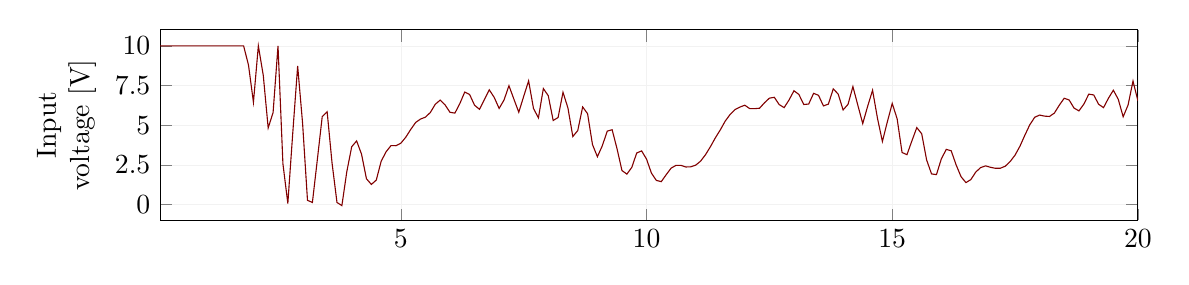
\begin{tikzpicture}
	\begin{axis}[
	ylabel style={align=center},
	ylabel= {Input\\voltage [V]},
	xmin=1, xmax=200,
	ymin=-1, ymax=11,
	legend style={font=\tiny},
	grid=both,
	grid style={line width=.1pt, draw=gray!10},
	width=14cm,height=4cm,
	xticklabels={0,5,10,15,20},xtick={0,50,100,150,200},
	ytick={0,2.5,5,7.5,10},
	%thick
	]
	\addplot[color=Maroon]
	coordinates {
(1,10)(2,10)(3,10)(4,10)(5,10)(6,10)(7,10)(8,10)(9,10)(10,10)(11,10)(12,10)(13,10)(14,10)(15,10)(16,10)(17,10)(18,10)(19,8.77604000000000)(20,6.44515000000000)(21,10)(22,8.14422000000000)(23,4.82346000000000)(24,5.79722000000000)(25,10)(26,2.57073000000000)(27,0.0660217000000000)(28,4.49288000000000)(29,8.72627000000000)(30,5.13007000000000)(31,0.263937000000000)(32,0.128117000000000)(33,2.81321000000000)(34,5.53795000000000)(35,5.84585000000000)(36,2.60796000000000)(37,0.129493000000000)(38,-0.0685393000000000)(39,2.06530000000000)(40,3.64148000000000)(41,4.00709000000000)(42,3.17044000000000)(43,1.62265000000000)(44,1.26422000000000)(45,1.53964000000000)(46,2.73199000000000)(47,3.32357000000000)(48,3.71353000000000)(49,3.70552000000000)(50,3.86339000000000)(51,4.23888000000000)(52,4.72440000000000)(53,5.16675000000000)(54,5.38401000000000)(55,5.50429000000000)(56,5.79872000000000)(57,6.31431000000000)(58,6.57895000000000)(59,6.27939000000000)(60,5.81235000000000)(61,5.75855000000000)(62,6.35690000000000)(63,7.08460000000000)(64,6.92943000000000)(65,6.25693000000000)(66,5.99871000000000)(67,6.60471000000000)(68,7.22559000000000)(69,6.74904000000000)(70,6.05317000000000)(71,6.58690000000000)(72,7.48733000000000)(73,6.64420000000000)(74,5.81527000000000)(75,6.81472000000000)(76,7.78960000000000)(77,6.04519000000000)(78,5.46141000000000)(79,7.30717000000000)(80,6.85774000000000)(81,5.29407000000000)(82,5.48309000000000)(83,7.07198000000000)(84,6.08641000000000)(85,4.28374000000000)(86,4.65718000000000)(87,6.14894000000000)(88,5.72430000000000)(89,3.77665000000000)(90,3.01151000000000)(91,3.70150000000000)(92,4.62425000000000)(93,4.71129000000000)(94,3.50690000000000)(95,2.13989000000000)(96,1.91542000000000)(97,2.33970000000000)(98,3.24670000000000)(99,3.37686000000000)(100,2.85972000000000)(101,1.97556000000000)(102,1.51801000000000)(103,1.44168000000000)(104,1.87972000000000)(105,2.29244000000000)(106,2.46888000000000)(107,2.46541000000000)(108,2.36429000000000)(109,2.37535000000000)(110,2.47754000000000)(111,2.73361000000000)(112,3.13877000000000)(113,3.64336000000000)(114,4.19858000000000)(115,4.69725000000000)(116,5.24855000000000)(117,5.67090000000000)(118,5.98177000000000)(119,6.13957000000000)(120,6.25763000000000)(121,6.04015000000000)(122,6.04019000000000)(123,6.06780000000000)(124,6.41003000000000)(125,6.70117000000000)(126,6.75482000000000)(127,6.29621000000000)(128,6.10534000000000)(129,6.58537000000000)(130,7.16684000000000)(131,6.93704000000000)(132,6.30238000000000)(133,6.32972000000000)(134,7.00783000000000)(135,6.87872000000000)(136,6.21411000000000)(137,6.32378000000000)(138,7.28606000000000)(139,6.96115000000000)(140,5.95959000000000)(141,6.30961000000000)(142,7.43149000000000)(143,6.25594000000000)(144,5.10238000000000)(145,6.18927000000000)(146,7.19836000000000)(147,5.42893000000000)(148,3.97497000000000)(149,5.20137000000000)(150,6.36700000000000)(151,5.40084000000000)(152,3.27898000000000)(153,3.13962000000000)(154,4.00707000000000)(155,4.84763000000000)(156,4.45546000000000)(157,2.80645000000000)(158,1.92799000000000)(159,1.88278000000000)(160,2.88051000000000)(161,3.47259000000000)(162,3.38484000000000)(163,2.50011000000000)(164,1.75593000000000)(165,1.38014000000000)(166,1.56946000000000)(167,2.04410000000000)(168,2.32836000000000)(169,2.43417000000000)(170,2.34476000000000)(171,2.28119000000000)(172,2.28597000000000)(173,2.41272000000000)(174,2.70679000000000)(175,3.11392000000000)(176,3.67994000000000)(177,4.37151000000000)(178,5.02784000000000)(179,5.49850000000000)(180,5.63624000000000)(181,5.56887000000000)(182,5.54811000000000)(183,5.76060000000000)(184,6.25883000000000)(185,6.69619000000000)(186,6.58704000000000)(187,6.07681000000000)(188,5.90013000000000)(189,6.32803000000000)(190,6.95418000000000)(191,6.90508000000000)(192,6.31842000000000)(193,6.10335000000000)(194,6.69580000000000)(195,7.20191000000000)(196,6.63133000000000)(197,5.52766000000000)(198,6.27185000000000)(199,7.77958000000000)(200,6.54071000000000)
	};
	
	\end{axis}
	\end{tikzpicture}
	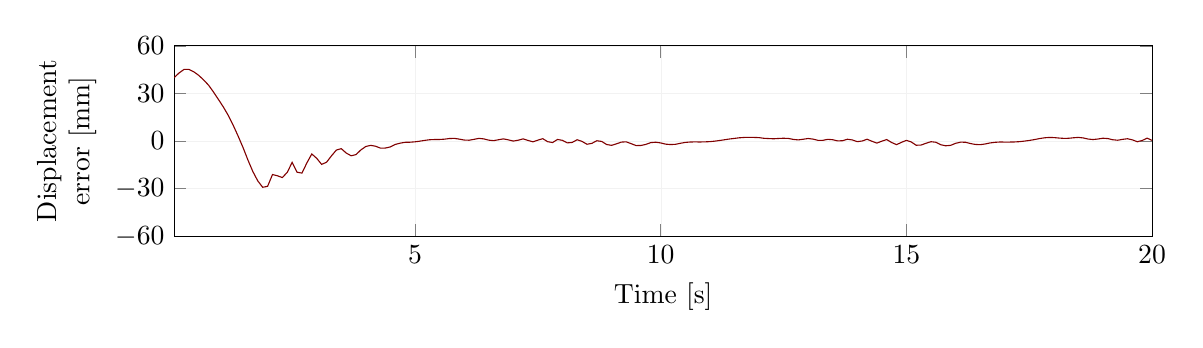
\begin{tikzpicture}
	\begin{axis}[
	ylabel style={align=center},
	ylabel={Displacement\\error [mm]},
	xlabel={Time [s]},
	xmin=1, xmax=200,
	ymin=-60, ymax=60,
	legend style={font=\tiny},
	grid=both,
	grid style={line width=.1pt, draw=gray!10},
	width=14cm,height=4cm,
	xticklabels={0,5,10,15,20},xtick={0,50,100,150,200},
	ytick={-60,-30,0,30,60},
	%thick
	]
	\addplot[color=Maroon]
	coordinates {
(1,40)(2,42.9250000000000)(3,45.1201000000000)(4,45.1356000000000)(5,43.6126000000000)(6,41.3428000000000)(7,38.4593000000000)(8,35.1665000000000)(9,30.8507000000000)(10,26.1998000000000)(11,21.4541000000000)(12,16.1362000000000)(13,9.95120000000001)(14,3.16670000000001)(15,-4.05650000000000)(16,-11.9552000000000)(17,-19.2028000000000)(18,-25.1001000000000)(19,-29.1446000000000)(20,-28.5610000000000)(21,-21.1211000000000)(22,-21.8937000000000)(23,-23.0251000000000)(24,-19.7488000000000)(25,-13.4461000000000)(26,-19.6558000000000)(27,-20.1950000000000)(28,-13.7486000000000)(29,-8.14040000000000)(30,-10.9225000000000)(31,-14.6964000000000)(32,-13.3626000000000)(33,-9.34120000000000)(34,-5.68240000000000)(35,-4.80620000000000)(36,-7.56350000000000)(37,-9.28560000000000)(38,-8.55510000000000)(39,-5.56570000000000)(40,-3.43300000000000)(41,-2.72410000000000)(42,-3.28830000000000)(43,-4.50730000000000)(44,-4.41500000000000)(45,-3.69810000000000)(46,-2.13590000000000)(47,-1.33070000000000)(48,-0.807700000000001)(49,-0.734900000000000)(50,-0.503599999999999)(51,-0.0777000000000001)(52,0.415600000000000)(53,0.816400000000000)(54,0.952000000000000)(55,0.977100000000000)(56,1.17380000000000)(57,1.57200000000000)(58,1.67940000000000)(59,1.21190000000000)(60,0.623700000000000)(61,0.507500000000000)(62,1.05510000000000)(63,1.67730000000000)(64,1.35440000000000)(65,0.546499999999995)(66,0.233600000000003)(67,0.816200000000002)(68,1.35550000000000)(69,0.743400000000001)(70,-0.0268000000000015)(71,0.509599999999999)(72,1.35910000000001)(73,0.380000000000003)(74,-0.486900000000006)(75,0.561200000000000)(76,1.48000000000000)(77,-0.412400000000005)(78,-0.954999999999998)(79,0.986300000000000)(80,0.438199999999995)(81,-1.16929999999999)(82,-0.863299999999995)(83,0.811900000000009)(84,-0.254799999999989)(85,-2.03200000000000)(86,-1.45540000000000)(87,0.181899999999999)(88,-0.260899999999999)(89,-2.18250000000000)(90,-2.72940000000000)(91,-1.76640000000000)(92,-0.667000000000002)(93,-0.513300000000001)(94,-1.66640000000000)(95,-2.86670000000000)(96,-2.80450000000000)(97,-2.09980000000000)(98,-0.982799999999998)(99,-0.754400000000000)(100,-1.19610000000000)(101,-1.96060000000000)(102,-2.22210000000000)(103,-2.07620000000000)(104,-1.43060000000000)(105,-0.874799999999999)(106,-0.610900000000001)(107,-0.553299999999998)(108,-0.599100000000000)(109,-0.528100000000000)(110,-0.373099999999999)(111,-0.0797000000000008)(112,0.333399999999999)(113,0.804700000000000)(114,1.27940000000000)(115,1.65010000000000)(116,2.03640000000000)(117,2.25510000000000)(118,2.34050000000000)(119,2.26420000000000)(120,2.15590000000000)(121,1.72280000000000)(122,1.55060000000000)(123,1.42310000000000)(124,1.62300000000000)(125,1.75190000000000)(126,1.63030000000000)(127,1.00870000000000)(128,0.716999999999999)(129,1.12530000000000)(130,1.59420000000000)(131,1.20500000000000)(132,0.449799999999996)(133,0.432200000000002)(134,1.06710000000000)(135,0.831299999999999)(136,0.0835000000000008)(137,0.184899999999999)(138,1.12860000000001)(139,0.690899999999999)(140,-0.379800000000003)(141,0.00820000000000221)(142,1.12930000000000)(143,-0.159199999999998)(144,-1.29680000000000)(145,-0.0802999999999940)(146,0.936899999999994)(147,-0.926299999999998)(148,-2.28760000000000)(149,-0.832400000000007)(150,0.416399999999996)(151,-0.591400000000000)(152,-2.65410000000000)(153,-2.52800000000000)(154,-1.40780000000000)(155,-0.426400000000001)(156,-0.775999999999996)(157,-2.34740000000000)(158,-2.99110000000000)(159,-2.73719999999999)(160,-1.46580000000000)(161,-0.727100000000004)(162,-0.742100000000001)(163,-1.55270000000000)(164,-2.14160000000000)(165,-2.30320000000000)(166,-1.88360000000000)(167,-1.22060000000000)(168,-0.814299999999999)(169,-0.627000000000001)(170,-0.653699999999999)(171,-0.651900000000001)(172,-0.582000000000001)(173,-0.397000000000000)(174,-0.0632000000000001)(175,0.350200000000001)(176,0.881200000000000)(177,1.48470000000000)(178,1.99250000000000)(179,2.26390000000000)(180,2.17530000000000)(181,1.89040000000000)(182,1.68060000000000)(183,1.72500000000000)(184,2.05070000000000)(185,2.28300000000000)(186,1.94560000000000)(187,1.24080000000000)(188,0.939999999999998)(189,1.27390000000000)(190,1.77270000000000)(191,1.54630000000000)(192,0.805000000000000)(193,0.509399999999999)(194,1.05100000000000)(195,1.45200000000000)(196,0.736200000000004)(197,-0.441099999999999)(198,0.347199999999994)(199,1.82020000000000)(200,0.399300000000011)
	};
	\end{axis}
	\end{tikzpicture}	
	\caption{Displacement control, 4.5 kilograms, 1 $\nicefrac{rad}{s}$}
	\label{fig:45kg-1rad}
\end{figure}

For each Figure, the first plot shows a comparison between the reference signal and
the effective displacement of the muscle. The second plot shows the voltage applied
to the input proportional valve. Lastly, the third plot shows the displacement error
in millimetres, that is the difference between the reference value and the muscle displacement.

As it is possible to see in Figure~\ref{fig:45kg-1rad} and~\ref{fig:45kg-2rad}, 
the reference tracking is very precise for 1 and 2 $\nicefrac{rad}{s}$.


On the other hand, it is possible to notice a steady degradation in performance
as the wave frequency rises. This is especially noticeable in Figure~\ref{fig:45kg-3rad},
for a sine wave with a frequency of 3 $\nicefrac{rad}{s}$,
where a significant delay of approximately 1 second can be appreciated
between the reference and the effective displacement.

\begin{figure}[H]
	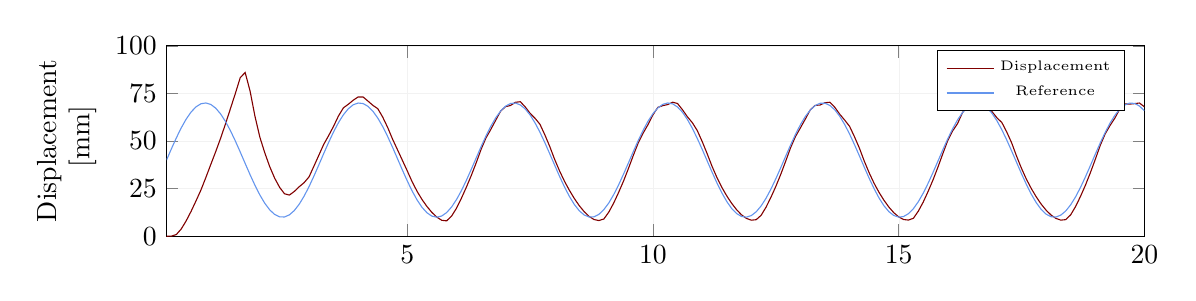
\begin{tikzpicture}
	\begin{axis}[
	ylabel style={align=center},
	ylabel={Displacement\\~[mm]},
	xmin=1, xmax=200,
	ymin=0, ymax=100,
	legend style={font=\tiny},
	grid=both,
	grid style={line width=.1pt, draw=gray!10},
	width=14cm,height=4cm,
	xticklabels={0,5,10,15,20},xtick={0,50,100,150,200},
	ytick={0,25,50,75,100},
	%thick
	]
	
	\addplot[
	color=Maroon
	]
	coordinates {
(1,0)(2,0.0700000000000000)(3,0.910000000000000)(4,3.84000000000000)(5,8.10000000000000)(6,13.0800000000000)(7,18.5800000000000)(8,24.2700000000000)(9,30.8300000000000)(10,37.6500000000000)(11,44.3700000000000)(12,51.4200000000000)(13,59.0200000000000)(14,66.9600000000000)(15,74.9500000000000)(16,83.2600000000000)(17,85.9900000000000)(18,76.2700000000000)(19,62.9500000000000)(20,51.9600000000000)(21,43.7600000000000)(22,36.5500000000000)(23,30.5300000000000)(24,25.7300000000000)(25,22.3100000000000)(26,21.6200000000000)(27,23.5200000000000)(28,25.9900000000000)(29,28.1400000000000)(30,31.1700000000000)(31,36.8200000000000)(32,42.5700000000000)(33,48.3000000000000)(34,52.8900000000000)(35,57.7800000000000)(36,63.2000000000000)(37,67.4400000000000)(38,69.3200000000000)(39,71.4400000000000)(40,73.1500000000000)(41,73.1300000000000)(42,70.9700000000000)(43,68.7300000000000)(44,66.9600000000000)(45,62.5400000000000)(46,57.1400000000000)(47,50.9900000000000)(48,45.4300000000000)(49,39.8600000000000)(50,34.2800000000000)(51,28.5100000000000)(52,23.5400000000000)(53,19.2600000000000)(54,15.6100000000000)(55,12.5200000000000)(56,10.0700000000000)(57,8.38000000000000)(58,8.08000000000000)(59,10.5500000000000)(60,14.6600000000000)(61,19.9000000000000)(62,25.6400000000000)(63,31.7900000000000)(64,38.4200000000000)(65,45.5300000000000)(66,51.5800000000000)(67,56.1400000000000)(68,60.9600000000000)(69,65.7400000000000)(70,68.0600000000000)(71,68.6700000000000)(72,70.3300000000000)(73,70.6500000000000)(74,67.9100000000000)(75,64.5000000000000)(76,61.9400000000000)(77,58.7700000000000)(78,53.2100000000000)(79,47.0600000000000)(80,40.2600000000000)(81,34.2200000000000)(82,28.8100000000000)(83,24.0600000000000)(84,19.7900000000000)(85,16.0400000000000)(86,12.8900000000000)(87,10.4100000000000)(88,8.78000000000000)(89,8.23000000000000)(90,9.07000000000000)(91,12.6500000000000)(92,17.4100000000000)(93,22.9900000000000)(94,28.9500000000000)(95,35.5600000000000)(96,42.4900000000000)(97,49.0500000000000)(98,54.2100000000000)(99,58.6700000000000)(100,63.7900000000000)(101,67.6900000000000)(102,68.5900000000000)(103,69.1500000000000)(104,70.3900000000000)(105,69.7000000000000)(106,66.4300000000000)(107,62.7300000000000)(108,59.6600000000000)(109,55.5500000000000)(110,49.8200000000000)(111,43.4900000000000)(112,36.8200000000000)(113,30.9100000000000)(114,25.7200000000000)(115,21.2400000000000)(116,17.3200000000000)(117,13.9800000000000)(118,11.2800000000000)(119,9.39000000000000)(120,8.43000000000000)(121,8.69000000000000)(122,10.9800000000000)(123,15.2300000000000)(124,20.4300000000000)(125,26.1800000000000)(126,32.5000000000000)(127,39.3800000000000)(128,46.4800000000000)(129,52.3900000000000)(130,56.9200000000000)(131,61.5400000000000)(132,66.3500000000000)(133,68.7300000000000)(134,68.9000000000000)(135,70.1300000000000)(136,70.3600000000000)(137,67.7200000000000)(138,64.0900000000000)(139,61.0300000000000)(140,57.7400000000000)(141,52.2700000000000)(142,46.3000000000000)(143,39.4300000000000)(144,33.2800000000000)(145,27.7800000000000)(146,23.0300000000000)(147,18.9100000000000)(148,15.3300000000000)(149,12.3900000000000)(150,10.1700000000000)(151,8.78000000000000)(152,8.50000000000000)(153,9.45000000000000)(154,13.1900000000000)(155,17.9600000000000)(156,23.6100000000000)(157,29.6500000000000)(158,36.3800000000000)(159,43.4800000000000)(160,50.3400000000000)(161,55.3900000000000)(162,59.2500000000000)(163,64.9800000000000)(164,68.1900000000000)(165,68.4900000000000)(166,69.6900000000000)(167,70.8600000000000)(168,69.0700000000000)(169,65.4300000000000)(170,62.1700000000000)(171,59.7000000000000)(172,54.7100000000000)(173,48.9800000000000)(174,41.9900000000000)(175,35.6100000000000)(176,29.9100000000000)(177,24.9800000000000)(178,20.6700000000000)(179,16.8600000000000)(180,13.7000000000000)(181,11.1400000000000)(182,9.37000000000000)(183,8.46000000000000)(184,8.72000000000000)(185,11.2500000000000)(186,15.5900000000000)(187,20.9200000000000)(188,26.7800000000000)(189,33.3000000000000)(190,40.2900000000000)(191,47.5800000000000)(192,53.6400000000000)(193,58.1100000000000)(194,62.0500000000000)(195,66.8500000000000)(196,69.4500000000000)(197,69.3900000000000)(198,69.6400000000000)(199,69.9700000000000)(200,67.9700000000000)
	};
	
	\addplot[color=CornflowerBlue]
	coordinates {
(1,40)(2,45.9601000000000)(3,51.6826000000000)(4,56.9393000000000)(5,61.5207000000000)(6,65.2441000000000)(7,67.9612000000000)(8,69.5635000000000)(9,69.9872000000000)(10,69.2154000000000)(11,67.2789000000000)(12,64.2549000000000)(13,60.2639000000000)(14,55.4650000000000)(15,50.0496000000000)(16,44.2336000000000)(17,38.2488000000000)(18,32.3338000000000)(19,26.7244000000000)(20,21.6443000000000)(21,17.2959000000000)(22,13.8527000000000)(23,11.4519000000000)(24,10.1893000000000)(25,10.1151000000000)(26,11.2323000000000)(27,13.4964000000000)(28,16.8171000000000)(29,21.0620000000000)(30,26.0619000000000)(31,31.6175000000000)(32,37.5073000000000)(33,43.4965000000000)(34,49.3462000000000)(35,54.8234000000000)(36,59.7096000000000)(37,63.8100000000000)(38,66.9612000000000)(39,69.0376000000000)(40,69.9563000000000)(41,69.6807000000000)(42,68.2219000000000)(43,65.6380000000000)(44,62.0319000000000)(45,57.5475000000000)(46,52.3636000000000)(47,46.6867000000000)(48,40.7433000000000)(49,34.7702000000000)(50,29.0056000000000)(51,23.6794000000000)(52,19.0038000000000)(53,15.1652000000000)(54,12.3167000000000)(55,10.5719000000000)(56,10.0003000000000)(57,10.6247000000000)(58,12.4201000000000)(59,15.3151000000000)(60,19.1942000000000)(61,23.9028000000000)(62,29.2531000000000)(63,35.0319000000000)(64,41.0087000000000)(65,46.9453000000000)(66,52.6050000000000)(67,57.7622000000000)(68,62.2113000000000)(69,65.7749000000000)(70,68.3109000000000)(71,69.7182000000000)(72,69.9408000000000)(73,68.9697000000000)(74,66.8437000000000)(75,63.6476000000000)(76,59.5086000000000)(77,54.5920000000000)(78,49.0936000000000)(79,43.2326000000000)(80,37.2428000000000)(81,31.3629000000000)(82,25.8273000000000)(83,20.8568000000000)(84,16.6494000000000)(85,13.3730000000000)(86,11.1581000000000)(87,10.0930000000000)(88,10.2202000000000)(89,11.5347000000000)(90,13.9839000000000)(91,17.4704000000000)(92,21.8550000000000)(93,26.9630000000000)(94,32.5908000000000)(95,38.5139000000000)(96,44.4963000000000)(97,50.2994000000000)(98,55.6920000000000)(99,60.4589000000000)(100,64.4102000000000)(101,67.3884000000000)(102,69.2746000000000)(103,69.9938000000000)(104,69.5172000000000)(105,67.8639000000000)(106,65.0997000000000)(107,61.3348000000000)(108,56.7195000000000)(109,51.4375000000000)(110,45.6996000000000)(111,39.7345000000000)(112,33.7799000000000)(113,28.0733000000000)(114,22.8422000000000)(115,18.2952000000000)(116,14.6134000000000)(117,11.9437000000000)(118,10.3925000000000)(119,10.0217000000000)(120,10.8460000000000)(121,12.8326000000000)(122,15.9023000000000)(123,19.9327000000000)(124,24.7631000000000)(125,30.2009000000000)(126,36.0294000000000)(127,42.0162000000000)(128,47.9227000000000)(129,53.5132000000000)(130,58.5651000000000)(131,62.8768000000000)(132,66.2764000000000)(133,68.6286000000000)(134,69.8393000000000)(135,69.8605000000000)(136,68.6913000000000)(137,66.3782000000000)(138,63.0135000000000)(139,58.7313000000000)(140,53.7024000000000)(141,48.1272000000000)(142,42.2280000000000)(143,36.2399000000000)(144,30.4018000000000)(145,24.9463000000000)(146,20.0910000000000)(147,16.0294000000000)(148,12.9234000000000)(149,10.8968000000000)(150,10.0305000000000)(151,10.3591000000000)(152,11.8692000000000)(153,14.5009000000000)(154,18.1492000000000)(155,22.6685000000000)(156,27.8789000000000)(157,33.5724000000000)(158,39.5222000000000)(159,45.4911000000000)(160,51.2410000000000)(161,56.5428000000000)(162,61.1851000000000)(163,64.9828000000000)(164,67.7845000000000)(165,69.4785000000000)(166,69.9974000000000)(167,69.3203000000000)(168,67.4743000000000)(169,64.5330000000000)(170,60.6136000000000)(171,55.8725000000000)(172,50.4985000000000)(173,44.7061000000000)(174,38.7260000000000)(175,32.7967000000000)(176,27.1545000000000)(177,22.0245000000000)(178,17.6111000000000)(179,14.0903000000000)(180,11.6024000000000)(181,10.2466000000000)(182,10.0770000000000)(183,11.1004000000000)(184,13.2759000000000)(185,16.5168000000000)(186,20.6939000000000)(187,25.6406000000000)(188,31.1599000000000)(189,37.0315000000000)(190,43.0215000000000)(191,48.8911000000000)(192,54.4061000000000)(193,59.3469000000000)(194,63.5164000000000)(195,66.7483000000000)(196,68.9139000000000)(197,69.9267000000000)(198,69.7465000000000)(199,68.3804000000000)(200,65.8828000000000)
	};
	
	\addlegendentry{Displacement}
	\addlegendentry{Reference}
	
	\end{axis}
	
	\end{tikzpicture}
	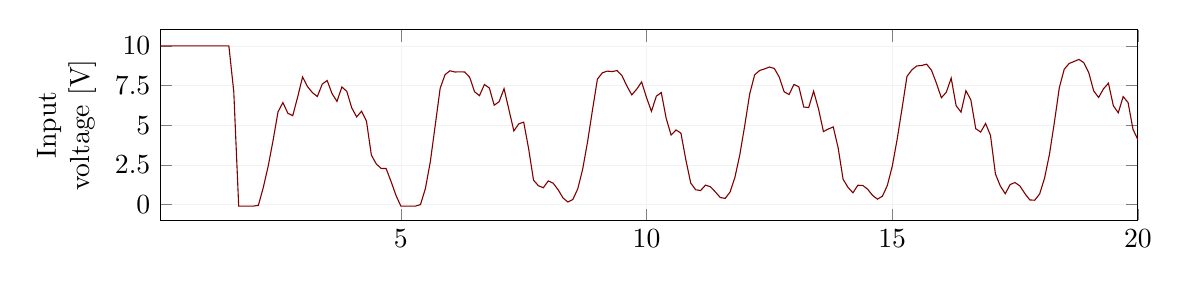
\begin{tikzpicture}
	\begin{axis}[
	ylabel style={align=center},
	ylabel= {Input\\voltage [V]},
	xmin=1, xmax=200,
	ymin=-1, ymax=11,
	legend style={font=\tiny},
	grid=both,
	grid style={line width=.1pt, draw=gray!10},
	width=14cm,height=4cm,
	xticklabels={0,5,10,15,20},xtick={0,50,100,150,200},
	ytick={0,2.5,5,7.5,10},
	%thick
	]
	\addplot[color=Maroon]
	coordinates {
(1,10)(2,10)(3,10)(4,10)(5,10)(6,10)(7,10)(8,10)(9,10)(10,10)(11,10)(12,10)(13,10)(14,10)(15,10)(16,7.10724000000000)(17,-0.100000000000000)(18,-0.100000000000000)(19,-0.100000000000000)(20,-0.100000000000000)(21,-0.0549542000000000)(22,1.06544000000000)(23,2.41492000000000)(24,4.04445000000000)(25,5.83617000000000)(26,6.42388000000000)(27,5.74920000000000)(28,5.59754000000000)(29,6.77518000000000)(30,8.03732000000000)(31,7.43211000000000)(32,7.05165000000000)(33,6.80454000000000)(34,7.58395000000000)(35,7.81673000000000)(36,6.98727000000000)(37,6.49867000000000)(38,7.40688000000000)(39,7.12735000000000)(40,6.09582000000000)(41,5.52090000000000)(42,5.87714000000000)(43,5.25838000000000)(44,3.11313000000000)(45,2.55592000000000)(46,2.27271000000000)(47,2.26821000000000)(48,1.45444000000000)(49,0.582704000000000)(50,-0.100000000000000)(51,-0.100000000000000)(52,-0.100000000000000)(53,-0.100000000000000)(54,-0.00333979000000000)(55,1.01251000000000)(56,2.69608000000000)(57,5.00349000000000)(58,7.32343000000000)(59,8.18244000000000)(60,8.42806000000000)(61,8.35005000000000)(62,8.36064000000000)(63,8.35071000000000)(64,8.02171000000000)(65,7.10718000000000)(66,6.85843000000000)(67,7.55812000000000)(68,7.34942000000000)(69,6.25812000000000)(70,6.47762000000000)(71,7.30006000000000)(72,5.96746000000000)(73,4.63747000000000)(74,5.08345000000000)(75,5.19065000000000)(76,3.52648000000000)(77,1.53667000000000)(78,1.18045000000000)(79,1.05787000000000)(80,1.48531000000000)(81,1.34370000000000)(82,0.932429000000000)(83,0.413623000000000)(84,0.155941000000000)(85,0.315436000000000)(86,0.983821000000000)(87,2.22555000000000)(88,3.95107000000000)(89,5.95954000000000)(90,7.89928000000000)(91,8.29712000000000)(92,8.40379000000000)(93,8.37631000000000)(94,8.44137000000000)(95,8.11859000000000)(96,7.46637000000000)(97,6.91013000000000)(98,7.26760000000000)(99,7.72273000000000)(100,6.73293000000000)(101,5.87309000000000)(102,6.82919000000000)(103,7.05682000000000)(104,5.42461000000000)(105,4.37399000000000)(106,4.69619000000000)(107,4.49832000000000)(108,2.81342000000000)(109,1.34743000000000)(110,0.928265000000000)(111,0.881085000000000)(112,1.22098000000000)(113,1.12039000000000)(114,0.795625000000000)(115,0.440775000000000)(116,0.384521000000000)(117,0.784174000000000)(118,1.72938000000000)(119,3.15982000000000)(120,5.00731000000000)(121,6.97552000000000)(122,8.16947000000000)(123,8.44208000000000)(124,8.54274000000000)(125,8.66390000000000)(126,8.57449000000000)(127,8.03423000000000)(128,7.10427000000000)(129,6.92910000000000)(130,7.56325000000000)(131,7.41946000000000)(132,6.14281000000000)(133,6.10758000000000)(134,7.13822000000000)(135,6.02335000000000)(136,4.59715000000000)(137,4.75719000000000)(138,4.88831000000000)(139,3.55848000000000)(140,1.58967000000000)(141,1.08071000000000)(142,0.737214000000000)(143,1.21198000000000)(144,1.20484000000000)(145,0.961541000000000)(146,0.572836000000000)(147,0.337307000000000)(148,0.523248000000000)(149,1.19605000000000)(150,2.40045000000000)(151,4.10501000000000)(152,6.05311000000000)(153,8.07172000000000)(154,8.48506000000000)(155,8.73035000000000)(156,8.76153000000000)(157,8.84197000000000)(158,8.45401000000000)(159,7.63708000000000)(160,6.72812000000000)(161,7.07002000000000)(162,7.96758000000000)(163,6.22879000000000)(164,5.82078000000000)(165,7.17427000000000)(166,6.59194000000000)(167,4.77560000000000)(168,4.56564000000000)(169,5.10477000000000)(170,4.35571000000000)(171,1.92892000000000)(172,1.16223000000000)(173,0.678600000000000)(174,1.26111000000000)(175,1.38540000000000)(176,1.16193000000000)(177,0.686357000000000)(178,0.287410000000000)(179,0.270698000000000)(180,0.665843000000000)(181,1.66032000000000)(182,3.17140000000000)(183,5.17545000000000)(184,7.35497000000000)(185,8.52145000000000)(186,8.88522000000000)(187,9.01237000000000)(188,9.14366000000000)(189,8.93330000000000)(190,8.30646000000000)(191,7.15915000000000)(192,6.74534000000000)(193,7.29272000000000)(194,7.64587000000000)(195,6.22444000000000)(196,5.77983000000000)(197,6.79908000000000)(198,6.42253000000000)(199,4.73706000000000)(200,4.08054000000000)
	};
	
	\end{axis}
	\end{tikzpicture}
	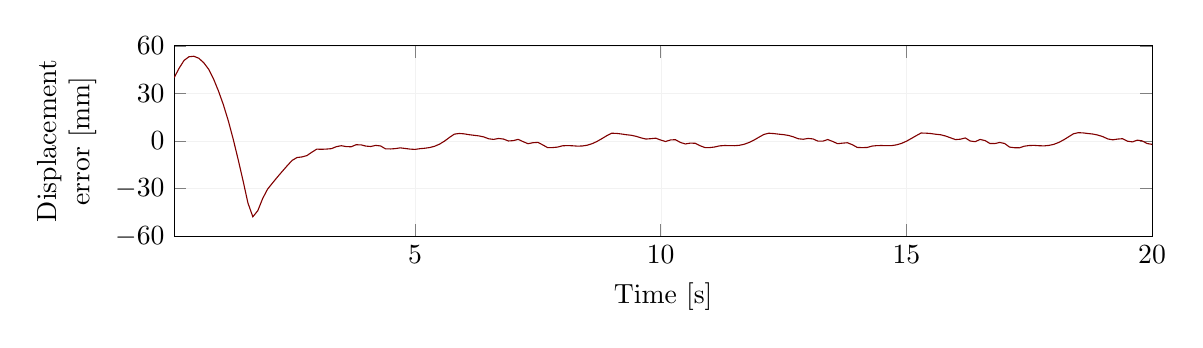
\begin{tikzpicture}
	\begin{axis}[
	ylabel style={align=center},
	ylabel={Displacement\\error [mm]},
	xlabel={Time [s]},
	xmin=1, xmax=200,
	ymin=-60, ymax=60,
	legend style={font=\tiny},
	grid=both,
	grid style={line width=.1pt, draw=gray!10},
	width=14cm,height=4cm,
	xticklabels={0,5,10,15,20},xtick={0,50,100,150,200},
	ytick={-60,-30,0,30,60},
	%thick
	]
	\addplot[color=Maroon]
	coordinates {
(1,40)(2,45.8901000000000)(3,50.7726000000000)(4,53.0993000000000)(5,53.4207000000000)(6,52.1641000000000)(7,49.3812000000000)(8,45.2935000000000)(9,39.1572000000000)(10,31.5654000000000)(11,22.9089000000000)(12,12.8349000000000)(13,1.24390000000000)(14,-11.4950000000000)(15,-24.9004000000000)(16,-39.0264000000000)(17,-47.7412000000000)(18,-43.9362000000000)(19,-36.2256000000000)(20,-30.3157000000000)(21,-26.4641000000000)(22,-22.6973000000000)(23,-19.0781000000000)(24,-15.5407000000000)(25,-12.1949000000000)(26,-10.3877000000000)(27,-10.0236000000000)(28,-9.17290000000000)(29,-7.07800000000000)(30,-5.10810000000000)(31,-5.20250000000000)(32,-5.06270000000000)(33,-4.80350000000000)(34,-3.54380000000000)(35,-2.95660000000000)(36,-3.49040000000000)(37,-3.63000000000000)(38,-2.35879999999999)(39,-2.40240000000000)(40,-3.19370000000001)(41,-3.44929999999999)(42,-2.74809999999999)(43,-3.09200000000000)(44,-4.92809999999999)(45,-4.99250000000000)(46,-4.77640000000000)(47,-4.30330000000000)(48,-4.68670000000000)(49,-5.08980000000000)(50,-5.27440000000000)(51,-4.83060000000000)(52,-4.53620000000000)(53,-4.09480000000000)(54,-3.29330000000000)(55,-1.94810000000000)(56,-0.0697000000000010)(57,2.24470000000000)(58,4.34010000000000)(59,4.76510000000000)(60,4.53420000000000)(61,4.00280000000000)(62,3.61310000000000)(63,3.24190000000000)(64,2.58870000000000)(65,1.41530000000000)(66,1.02500000000000)(67,1.62220000000000)(68,1.25130000000000)(69,0.0349000000000075)(70,0.250900000000001)(71,1.04819999999999)(72,-0.389200000000002)(73,-1.68030000000000)(74,-1.06630000000000)(75,-0.852400000000003)(76,-2.43140000000000)(77,-4.17800000000000)(78,-4.11640000000000)(79,-3.82740000000000)(80,-3.01720000000000)(81,-2.85710000000000)(82,-2.98270000000000)(83,-3.20320000000000)(84,-3.14060000000000)(85,-2.66700000000000)(86,-1.73190000000000)(87,-0.317000000000000)(88,1.44020000000000)(89,3.30470000000000)(90,4.91390000000000)(91,4.82040000000000)(92,4.44500000000000)(93,3.97300000000000)(94,3.64080000000000)(95,2.95390000000000)(96,2.00630000000000)(97,1.24940000000000)(98,1.48200000000000)(99,1.78890000000000)(100,0.620200000000004)(101,-0.301599999999993)(102,0.684600000000003)(103,0.843799999999987)(104,-0.872799999999998)(105,-1.83610000000000)(106,-1.33030000000001)(107,-1.39520000000000)(108,-2.94050000000000)(109,-4.11250000000000)(110,-4.12040000000000)(111,-3.75550000000001)(112,-3.04010000000000)(113,-2.83670000000000)(114,-2.87780000000000)(115,-2.94480000000000)(116,-2.70660000000000)(117,-2.03630000000000)(118,-0.887499999999999)(119,0.631699999999999)(120,2.41600000000000)(121,4.14260000000000)(122,4.92230000000000)(123,4.70270000000000)(124,4.33310000000000)(125,4.02090000000000)(126,3.52940000000000)(127,2.63620000000000)(128,1.44270000000000)(129,1.12320000000000)(130,1.64510000000000)(131,1.33680000000000)(132,-0.0735999999999990)(133,-0.101399999999998)(134,0.939299999999989)(135,-0.269499999999994)(136,-1.66870000000000)(137,-1.34179999999999)(138,-1.07650000000000)(139,-2.29870000000000)(140,-4.03760000000001)(141,-4.14280000000000)(142,-4.07200000000000)(143,-3.19010000000000)(144,-2.87820000000000)(145,-2.83370000000000)(146,-2.93900000000000)(147,-2.88060000000000)(148,-2.40660000000000)(149,-1.49320000000000)(150,-0.139500000000000)(151,1.57910000000000)(152,3.36920000000000)(153,5.05090000000000)(154,4.95920000000000)(155,4.70850000000000)(156,4.26890000000000)(157,3.92240000000000)(158,3.14220000000000)(159,2.01110000000001)(160,0.900999999999996)(161,1.15280000000000)(162,1.93510000000000)(163,0.00279999999999347)(164,-0.405500000000004)(165,0.988500000000002)(166,0.307400000000001)(167,-1.53970000000000)(168,-1.59569999999999)(169,-0.897000000000006)(170,-1.55640000000000)(171,-3.82750000000000)(172,-4.21150000000000)(173,-4.27390000000000)(174,-3.26400000000000)(175,-2.81330000000000)(176,-2.75550000000000)(177,-2.95550000000000)(178,-3.05890000000000)(179,-2.76970000000000)(180,-2.09760000000000)(181,-0.893400000000000)(182,0.707000000000001)(183,2.64040000000000)(184,4.55590000000000)(185,5.26680000000000)(186,5.10390000000000)(187,4.72060000000000)(188,4.37990000000000)(189,3.73150000000000)(190,2.73150000000000)(191,1.31110000000000)(192,0.766100000000002)(193,1.23690000000000)(194,1.46640000000000)(195,-0.101699999999994)(196,-0.536100000000005)(197,0.536699999999996)(198,0.106499999999997)(199,-1.58960000000000)(200,-2.08720000000000)
	};
	\end{axis}
	\end{tikzpicture}	
	\caption{Displacement control, 4.5 kilograms, 2 $\nicefrac{rad}{s}$}
	\label{fig:45kg-2rad}
\end{figure}

\begin{figure}[H]
	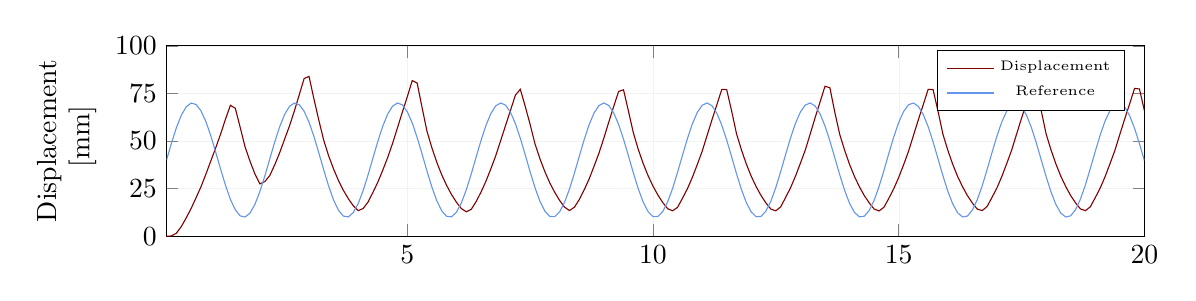
\begin{tikzpicture}
	\begin{axis}[
	ylabel style={align=center},
	ylabel={Displacement\\~[mm]},
	xmin=1, xmax=200,
	ymin=0, ymax=100,
	legend style={font=\tiny},
	grid=both,
	grid style={line width=.1pt, draw=gray!10},
	width=14cm,height=4cm,
	xticklabels={0,5,10,15,20},xtick={0,50,100,150,200},
	ytick={0,25,50,75,100},
	%thick
	]
	
	\addplot[
	color=Maroon
	]
	coordinates {
(1,0)(2,0.140000000000000)(3,1.60000000000000)(4,5.07000000000000)(5,9.61000000000000)(6,14.5700000000000)(7,20.1600000000000)(8,25.9200000000000)(9,32.5300000000000)(10,39.4700000000000)(11,46.3600000000000)(12,53.6400000000000)(13,61.4700000000000)(14,68.7700000000000)(15,67.1600000000000)(16,57.0800000000000)(17,46.7900000000000)(18,39.3100000000000)(19,32.6200000000000)(20,27.5100000000000)(21,28.6900000000000)(22,31.8400000000000)(23,37.3900000000000)(24,43.7000000000000)(25,50.7800000000000)(26,57.7600000000000)(27,65.6400000000000)(28,74.2200000000000)(29,82.8200000000000)(30,83.9400000000000)(31,72.0500000000000)(32,60.8500000000000)(33,50.3100000000000)(34,42.1600000000000)(35,35.2600000000000)(36,29.2100000000000)(37,24.0700000000000)(38,19.6800000000000)(39,16.0100000000000)(40,13.4500000000000)(41,14.5500000000000)(42,17.9300000000000)(43,22.9900000000000)(44,28.4000000000000)(45,34.6500000000000)(46,41.3200000000000)(47,48.7600000000000)(48,56.9700000000000)(49,65.2500000000000)(50,73.2800000000000)(51,81.7400000000000)(52,80.5000000000000)(53,67.6500000000000)(54,55.1300000000000)(55,46.4900000000000)(56,38.8200000000000)(57,32.2700000000000)(58,26.7300000000000)(59,21.8900000000000)(60,17.8600000000000)(61,14.5300000000000)(62,12.8600000000000)(63,14.0900000000000)(64,18.2000000000000)(65,23.1800000000000)(66,28.8800000000000)(67,35.4000000000000)(68,42.3200000000000)(69,50.2500000000000)(70,58.2100000000000)(71,66.1300000000000)(72,74.1200000000000)(73,77.1600000000000)(74,68.1700000000000)(75,58.6900000000000)(76,48.4100000000000)(77,40.6200000000000)(78,33.8700000000000)(79,27.9900000000000)(80,23.0400000000000)(81,18.7800000000000)(82,15.2900000000000)(83,13.4900000000000)(84,15.2400000000000)(85,19.2500000000000)(86,24.3800000000000)(87,30.0600000000000)(88,36.7200000000000)(89,43.6100000000000)(90,51.5600000000000)(91,59.9700000000000)(92,68.1000000000000)(93,76.0600000000000)(94,76.9100000000000)(95,65.7700000000000)(96,54.3300000000000)(97,45.6100000000000)(98,38.1900000000000)(99,31.8000000000000)(100,26.3300000000000)(101,21.6200000000000)(102,17.6600000000000)(103,14.4300000000000)(104,13.3600000000000)(105,15.1800000000000)(106,19.9600000000000)(107,24.9400000000000)(108,30.8700000000000)(109,37.5700000000000)(110,44.5600000000000)(111,52.8700000000000)(112,61.1400000000000)(113,69.1100000000000)(114,77.1200000000000)(115,77)(116,65.8200000000000)(117,53.7900000000000)(118,45.3400000000000)(119,37.8800000000000)(120,31.4400000000000)(121,26.0200000000000)(122,21.3300000000000)(123,17.4100000000000)(124,14.2300000000000)(125,13.3500000000000)(126,15.4800000000000)(127,20.4500000000000)(128,25.5100000000000)(129,31.5600000000000)(130,38.3300000000000)(131,45.3500000000000)(132,53.7200000000000)(133,62.3500000000000)(134,70.5100000000000)(135,78.7500000000000)(136,77.9900000000000)(137,65.1000000000000)(138,53.4800000000000)(139,45.1500000000000)(140,37.7300000000000)(141,31.4000000000000)(142,26.0200000000000)(143,21.3600000000000)(144,17.5000000000000)(145,14.3200000000000)(146,13.2800000000000)(147,15.2100000000000)(148,19.9500000000000)(149,24.9600000000000)(150,30.8700000000000)(151,37.5300000000000)(152,44.5800000000000)(153,52.9200000000000)(154,61.1700000000000)(155,69.0900000000000)(156,77.1600000000000)(157,77)(158,65.6900000000000)(159,53.5800000000000)(160,45.1900000000000)(161,37.7500000000000)(162,31.3500000000000)(163,25.9700000000000)(164,21.2900000000000)(165,17.4100000000000)(166,14.2400000000000)(167,13.4800000000000)(168,15.6600000000000)(169,20.4400000000000)(170,25.4200000000000)(171,31.4600000000000)(172,38.2400000000000)(173,45.3100000000000)(174,53.7000000000000)(175,61.9400000000000)(176,69.9200000000000)(177,78.0700000000000)(178,77.6300000000000)(179,66.0400000000000)(180,53.7700000000000)(181,45.3500000000000)(182,37.9100000000000)(183,31.4800000000000)(184,26.0800000000000)(185,21.3800000000000)(186,17.5000000000000)(187,14.3200000000000)(188,13.4400000000000)(189,15.4600000000000)(190,20.2400000000000)(191,25.2400000000000)(192,31.2600000000000)(193,38.0700000000000)(194,45.0900000000000)(195,53.4300000000000)(196,61.6200000000000)(197,69.5000000000000)(198,77.6200000000000)(199,77.3400000000000)(200,65.9800000000000)
	};
	
	\addplot[color=CornflowerBlue]
	coordinates {
(1,40)(2,48.8656000000000)(3,56.9393000000000)(4,63.4998000000000)(5,67.9612000000000)(6,69.9248000000000)(7,69.2154000000000)(8,65.8963000000000)(9,60.2639000000000)(10,52.8214000000000)(11,44.2336000000000)(12,35.2676000000000)(13,26.7244000000000)(14,19.3670000000000)(15,13.8527000000000)(16,10.6741000000000)(17,10.1151000000000)(18,12.2256000000000)(19,16.8171000000000)(20,23.4794000000000)(21,31.6175000000000)(22,40.5044000000000)(23,49.3462000000000)(24,57.3532000000000)(25,63.8100000000000)(26,68.1400000000000)(27,69.9563000000000)(28,69.0967000000000)(29,65.6380000000000)(30,59.8891000000000)(31,52.3636000000000)(32,43.7336000000000)(33,34.7702000000000)(34,26.2739000000000)(35,19.0038000000000)(36,13.6091000000000)(37,10.5719000000000)(38,10.1634000000000)(39,12.4201000000000)(40,17.1405000000000)(41,23.9028000000000)(42,32.1030000000000)(43,41.0087000000000)(44,49.8242000000000)(45,57.7622000000000)(46,64.1135000000000)(47,68.3109000000000)(48,69.9793000000000)(49,68.9697000000000)(50,65.3724000000000)(51,59.5086000000000)(52,51.9022000000000)(53,43.2326000000000)(54,34.2742000000000)(55,25.8273000000000)(56,18.6464000000000)(57,13.3730000000000)(58,10.4780000000000)(59,10.2202000000000)(60,12.6225000000000)(61,17.4704000000000)(62,24.3307000000000)(63,32.5908000000000)(64,41.5127000000000)(65,50.2994000000000)(66,58.1662000000000)(67,64.4102000000000)(68,68.4737000000000)(69,69.9938000000000)(70,68.8346000000000)(71,65.0997000000000)(72,59.1227000000000)(73,51.4375000000000)(74,42.7307000000000)(75,33.7799000000000)(76,25.3848000000000)(77,18.2952000000000)(78,13.1444000000000)(79,10.3925000000000)(80,10.2854000000000)(81,12.8326000000000)(82,17.8066000000000)(83,24.7631000000000)(84,33.0806000000000)(85,42.0162000000000)(86,50.7718000000000)(87,58.5651000000000)(88,64.7000000000000)(89,68.6286000000000)(90,69.9998000000000)(91,68.6913000000000)(92,64.8198000000000)(93,58.7313000000000)(94,50.9696000000000)(95,42.2280000000000)(96,33.2873000000000)(97,24.9463000000000)(98,17.9500000000000)(99,12.9234000000000)(100,10.3154000000000)(101,10.3591000000000)(102,13.0505000000000)(103,18.1492000000000)(104,25.1998000000000)(105,33.5724000000000)(106,42.5192000000000)(107,51.2410000000000)(108,58.9587000000000)(109,64.9828000000000)(110,68.7753000000000)(111,69.9974000000000)(112,68.5399000000000)(113,64.5330000000000)(114,58.3347000000000)(115,50.4985000000000)(116,41.7246000000000)(117,32.7967000000000)(118,24.5121000000000)(119,17.6111000000000)(120,12.7100000000000)(121,10.2466000000000)(122,10.4410000000000)(123,13.2759000000000)(124,18.4979000000000)(125,25.6406000000000)(126,34.0660000000000)(127,43.0215000000000)(128,51.7071000000000)(129,59.3469000000000)(130,65.2585000000000)(131,68.9139000000000)(132,69.9864000000000)(133,68.3804000000000)(134,64.2392000000000)(135,57.9328000000000)(136,50.0245000000000)(137,41.2208000000000)(138,32.3080000000000)(139,24.0823000000000)(140,17.2785000000000)(141,12.5044000000000)(142,10.1863000000000)(143,10.5314000000000)(144,13.5089000000000)(145,18.8527000000000)(146,26.0855000000000)(147,34.5613000000000)(148,43.5229000000000)(149,52.1699000000000)(150,59.7297000000000)(151,65.5271000000000)(152,69.0443000000000)(153,69.9670000000000)(154,68.2129000000000)(155,63.9386000000000)(156,57.5259000000000)(157,49.5477000000000)(158,40.7166000000000)(159,31.8215000000000)(160,23.6570000000000)(161,16.9524000000000)(162,12.3065000000000)(163,10.1344000000000)(164,10.6301000000000)(165,13.7493000000000)(166,19.2135000000000)(167,26.5344000000000)(168,35.0582000000000)(169,44.0234000000000)(170,52.6292000000000)(171,60.1069000000000)(172,65.7885000000000)(173,69.1665000000000)(174,69.9391000000000)(175,68.0374000000000)(176,63.6312000000000)(177,57.1140000000000)(178,49.0682000000000)(179,40.2123000000000)(180,31.3374000000000)(181,23.2363000000000)(182,16.6327000000000)(183,12.1164000000000)(184,10.0909000000000)(185,10.7371000000000)(186,13.9972000000000)(187,19.5801000000000)(188,26.9870000000000)(189,35.5564000000000)(190,44.5227000000000)(191,53.0849000000000)(192,60.4784000000000)(193,66.0426000000000)(194,69.2804000000000)(195,69.9028000000000)(196,67.8540000000000)(197,63.3171000000000)(198,56.6973000000000)(199,48.5861000000000)(200,39.7078000000000)
	};
	
	\addlegendentry{Displacement}
	\addlegendentry{Reference}
	
	\end{axis}
	
	\end{tikzpicture}
	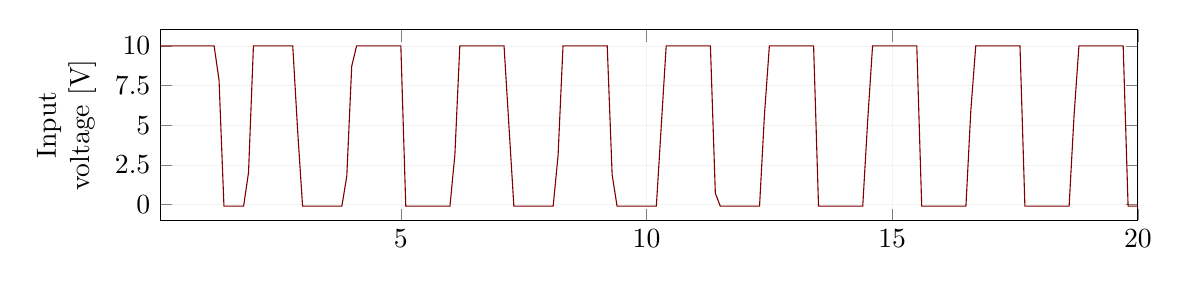
\begin{tikzpicture}
	\begin{axis}[
	ylabel style={align=center},
	ylabel= {Input\\voltage [V]},
	xmin=1, xmax=200,
	ymin=-1, ymax=11,
	legend style={font=\tiny},
	grid=both,
	grid style={line width=.1pt, draw=gray!10},
	width=14cm,height=4cm,
	xticklabels={0,5,10,15,20},xtick={0,50,100,150,200},
	ytick={0,2.5,5,7.5,10},
	%thick
	]
	\addplot[color=Maroon]
	coordinates {
(1,10)(2,10)(3,10)(4,10)(5,10)(6,10)(7,10)(8,10)(9,10)(10,10)(11,10)(12,10)(13,7.83628000000000)(14,-0.100000000000000)(15,-0.100000000000000)(16,-0.100000000000000)(17,-0.100000000000000)(18,-0.100000000000000)(19,2.01684000000000)(20,10)(21,10)(22,10)(23,10)(24,10)(25,10)(26,10)(27,10)(28,10)(29,4.63484000000000)(30,-0.100000000000000)(31,-0.100000000000000)(32,-0.100000000000000)(33,-0.100000000000000)(34,-0.100000000000000)(35,-0.100000000000000)(36,-0.100000000000000)(37,-0.100000000000000)(38,-0.100000000000000)(39,1.79367000000000)(40,8.71503000000000)(41,10)(42,10)(43,10)(44,10)(45,10)(46,10)(47,10)(48,10)(49,10)(50,10)(51,-0.100000000000000)(52,-0.100000000000000)(53,-0.100000000000000)(54,-0.100000000000000)(55,-0.100000000000000)(56,-0.100000000000000)(57,-0.100000000000000)(58,-0.100000000000000)(59,-0.100000000000000)(60,-0.100000000000000)(61,3.15918000000000)(62,10)(63,10)(64,10)(65,10)(66,10)(67,10)(68,10)(69,10)(70,10)(71,10)(72,4.93470000000000)(73,-0.100000000000000)(74,-0.100000000000000)(75,-0.100000000000000)(76,-0.100000000000000)(77,-0.100000000000000)(78,-0.100000000000000)(79,-0.100000000000000)(80,-0.100000000000000)(81,-0.100000000000000)(82,3.10423000000000)(83,10)(84,10)(85,10)(86,10)(87,10)(88,10)(89,10)(90,10)(91,10)(92,10)(93,1.87619000000000)(94,-0.100000000000000)(95,-0.100000000000000)(96,-0.100000000000000)(97,-0.100000000000000)(98,-0.100000000000000)(99,-0.100000000000000)(100,-0.100000000000000)(101,-0.100000000000000)(102,-0.100000000000000)(103,4.97213000000000)(104,10)(105,10)(106,10)(107,10)(108,10)(109,10)(110,10)(111,10)(112,10)(113,10)(114,0.715465000000000)(115,-0.100000000000000)(116,-0.100000000000000)(117,-0.100000000000000)(118,-0.100000000000000)(119,-0.100000000000000)(120,-0.100000000000000)(121,-0.100000000000000)(122,-0.100000000000000)(123,-0.100000000000000)(124,5.66883000000000)(125,10)(126,10)(127,10)(128,10)(129,10)(130,10)(131,10)(132,10)(133,10)(134,10)(135,-0.100000000000000)(136,-0.100000000000000)(137,-0.100000000000000)(138,-0.100000000000000)(139,-0.100000000000000)(140,-0.100000000000000)(141,-0.100000000000000)(142,-0.100000000000000)(143,-0.100000000000000)(144,-0.100000000000000)(145,5.26525000000000)(146,10)(147,10)(148,10)(149,10)(150,10)(151,10)(152,10)(153,10)(154,10)(155,10)(156,-0.100000000000000)(157,-0.100000000000000)(158,-0.100000000000000)(159,-0.100000000000000)(160,-0.100000000000000)(161,-0.100000000000000)(162,-0.100000000000000)(163,-0.100000000000000)(164,-0.100000000000000)(165,-0.100000000000000)(166,5.94434000000000)(167,10)(168,10)(169,10)(170,10)(171,10)(172,10)(173,10)(174,10)(175,10)(176,10)(177,-0.100000000000000)(178,-0.100000000000000)(179,-0.100000000000000)(180,-0.100000000000000)(181,-0.100000000000000)(182,-0.100000000000000)(183,-0.100000000000000)(184,-0.100000000000000)(185,-0.100000000000000)(186,-0.100000000000000)(187,5.59605000000000)(188,10)(189,10)(190,10)(191,10)(192,10)(193,10)(194,10)(195,10)(196,10)(197,10)(198,-0.100000000000000)(199,-0.100000000000000)(200,-0.100000000000000)
	};
	
	\end{axis}
	\end{tikzpicture}
	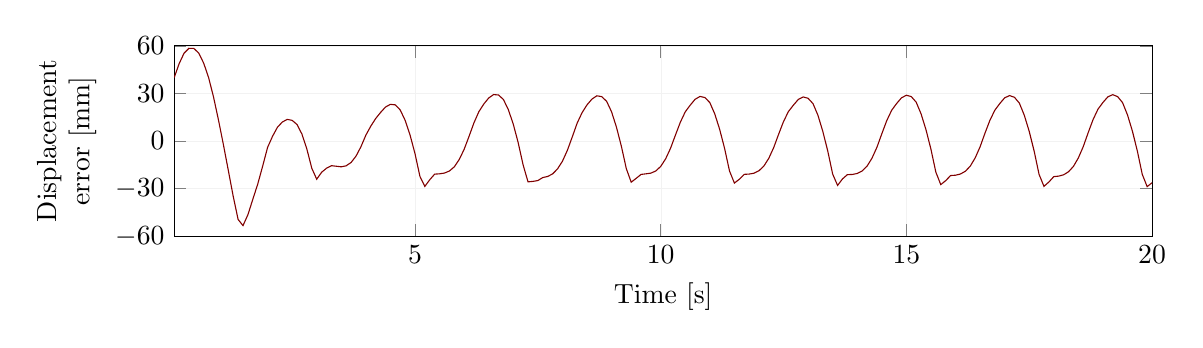
\begin{tikzpicture}
	\begin{axis}[
	ylabel style={align=center},
	ylabel={Displacement\\error [mm]},
	xlabel={Time [s]},
	xmin=1, xmax=200,
	ymin=-60, ymax=60,
	legend style={font=\tiny},
	grid=both,
	grid style={line width=.1pt, draw=gray!10},
	width=14cm,height=4cm,
	xticklabels={0,5,10,15,20},xtick={0,50,100,150,200},
	ytick={-60,-30,0,30,60},
	%thick
	]
	\addplot[color=Maroon]
	coordinates {
(1,40)(2,48.7256000000000)(3,55.3393000000000)(4,58.4298000000000)(5,58.3512000000000)(6,55.3548000000000)(7,49.0554000000000)(8,39.9763000000000)(9,27.7339000000000)(10,13.3514000000000)(11,-2.12640000000000)(12,-18.3724000000000)(13,-34.7456000000000)(14,-49.4030000000000)(15,-53.3073000000000)(16,-46.4059000000000)(17,-36.6749000000000)(18,-27.0844000000000)(19,-15.8029000000000)(20,-4.03060000000000)(21,2.92750000000000)(22,8.66440000000000)(23,11.9562000000000)(24,13.6532000000000)(25,13.0300000000000)(26,10.3800000000000)(27,4.31630000000000)(28,-5.12330000000000)(29,-17.1820000000000)(30,-24.0509000000000)(31,-19.6864000000000)(32,-17.1164000000000)(33,-15.5398000000000)(34,-15.8861000000000)(35,-16.2562000000000)(36,-15.6009000000000)(37,-13.4981000000000)(38,-9.51660000000000)(39,-3.58990000000000)(40,3.69050000000000)(41,9.35280000000000)(42,14.1730000000000)(43,18.0187000000000)(44,21.4242000000000)(45,23.1122000000000)(46,22.7935000000000)(47,19.5509000000000)(48,13.0093000000000)(49,3.71970000000000)(50,-7.90760000000000)(51,-22.2314000000000)(52,-28.5978000000000)(53,-24.4174000000000)(54,-20.8558000000000)(55,-20.6627000000000)(56,-20.1736000000000)(57,-18.8970000000000)(58,-16.2520000000000)(59,-11.6698000000000)(60,-5.23750000000000)(61,2.94040000000000)(62,11.4707000000000)(63,18.5008000000000)(64,23.3127000000000)(65,27.1194000000000)(66,29.2862000000000)(67,29.0102000000000)(68,26.1537000000000)(69,19.7438000000000)(70,10.6246000000000)(71,-1.03030000000000)(72,-14.9973000000000)(73,-25.7225000000000)(74,-25.4393000000000)(75,-24.9101000000000)(76,-23.0252000000000)(77,-22.3248000000000)(78,-20.7256000000000)(79,-17.5975000000000)(80,-12.7546000000000)(81,-5.94740000000000)(82,2.51660000000000)(83,11.2731000000000)(84,17.8406000000000)(85,22.7662000000000)(86,26.3918000000000)(87,28.5051000000000)(88,27.9800000000000)(89,25.0186000000000)(90,18.4398000000000)(91,8.72130000000000)(92,-3.28019999999999)(93,-17.3287000000000)(94,-25.9404000000000)(95,-23.5420000000000)(96,-21.0427000000000)(97,-20.6637000000000)(98,-20.2400000000000)(99,-18.8766000000000)(100,-16.0146000000000)(101,-11.2609000000000)(102,-4.60950000000000)(103,3.71920000000000)(104,11.8398000000000)(105,18.3924000000000)(106,22.5592000000000)(107,26.3010000000000)(108,28.0887000000000)(109,27.4128000000000)(110,24.2153000000000)(111,17.1274000000000)(112,7.39990000000000)(113,-4.57700000000000)(114,-18.7853000000000)(115,-26.5015000000000)(116,-24.0954000000000)(117,-20.9933000000000)(118,-20.8279000000000)(119,-20.2689000000000)(120,-18.7300000000000)(121,-15.7734000000000)(122,-10.8890000000000)(123,-4.13410000000000)(124,4.26790000000000)(125,12.2906000000000)(126,18.5860000000000)(127,22.5715000000000)(128,26.1971000000000)(129,27.7869000000000)(130,26.9285000000000)(131,23.5639000000000)(132,16.2664000000000)(133,6.03039999999999)(134,-6.27080000000001)(135,-20.8172000000000)(136,-27.9655000000000)(137,-23.8792000000000)(138,-21.1720000000000)(139,-21.0677000000000)(140,-20.4515000000000)(141,-18.8956000000000)(142,-15.8337000000000)(143,-10.8286000000000)(144,-3.99110000000000)(145,4.53270000000000)(146,12.8055000000000)(147,19.3513000000000)(148,23.5729000000000)(149,27.2099000000000)(150,28.8597000000000)(151,27.9971000000000)(152,24.4643000000000)(153,17.0470000000000)(154,7.04290000000000)(155,-5.15140000000000)(156,-19.6341000000000)(157,-27.4523000000000)(158,-24.9734000000000)(159,-21.7585000000000)(160,-21.5330000000000)(161,-20.7976000000000)(162,-19.0435000000000)(163,-15.8356000000000)(164,-10.6599000000000)(165,-3.66070000000000)(166,4.97350000000000)(167,13.0544000000000)(168,19.3982000000000)(169,23.5834000000000)(170,27.2092000000000)(171,28.6469000000000)(172,27.5485000000000)(173,23.8565000000000)(174,16.2391000000000)(175,6.09740000000001)(176,-6.28880000000000)(177,-20.9560000000000)(178,-28.5618000000000)(179,-25.8277000000000)(180,-22.4326000000000)(181,-22.1137000000000)(182,-21.2773000000000)(183,-19.3636000000000)(184,-15.9891000000000)(185,-10.6429000000000)(186,-3.50280000000000)(187,5.26010000000000)(188,13.5470000000000)(189,20.0964000000000)(190,24.2827000000000)(191,27.8449000000000)(192,29.2184000000000)(193,27.9726000000000)(194,24.1904000000000)(195,16.4728000000000)(196,6.23400000000000)(197,-6.18290000000000)(198,-20.9227000000000)(199,-28.7539000000000)(200,-26.2722000000000)
	};
	\end{axis}
	\end{tikzpicture}	
	\caption{Displacement control, 4.5 kilograms, 3 $\nicefrac{rad}{s}$}
	\label{fig:45kg-3rad}
\end{figure}

%7.5
\subsubsection{Application on Muscle -- 7 Kilograms Weight}
\label{sec:6.7kg}

This Section covers the application of PI control on a real McKibben artificial muscle
driven by tap-water. The weight attached to the muscle weighs 4.5 kilograms.

The PID gains have been set as those of Table~\ref{tab:pid_gains_45}
for all three frequencies, to study the effect of the weight on control performances.

The main difference between the control performance with a weight of 4.5 kilograms
is the case with a reference with frequency of 3 $\nicefrac{rad}{s}$.
Although there is still a relevant error due to the delay in following the reference,
it has lower impact on the control performance, meaning that the displacement error
is lower. This is probably due to the greater inertia caused by the heavier weight.
It is possible to appreciate these differences in Figure~\ref{fig:7kg-3rad}.

\begin{figure}[H]
	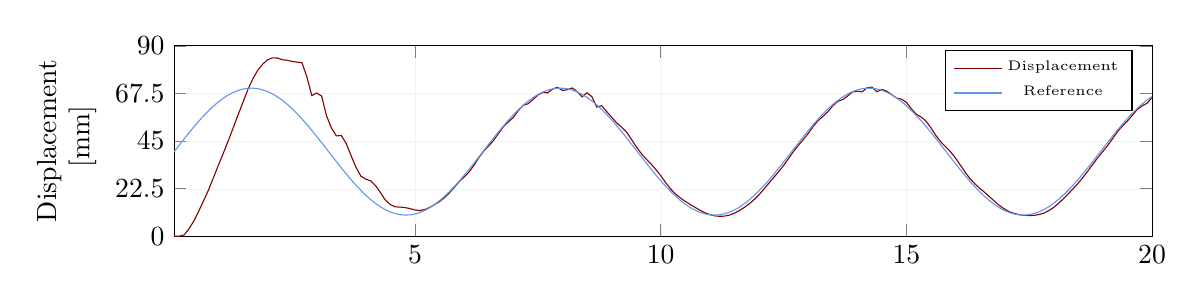
\begin{tikzpicture}
	\begin{axis}[
	ylabel style={align=center},
	ylabel={Displacement\\~[mm]},
	xmin=1, xmax=200,
	ymin=0, ymax=90,
	legend style={font=\tiny},
	grid=both,
	grid style={line width=.1pt, draw=gray!10},
	width=14cm,height=4cm,
	xticklabels={0,5,10,15,20},xtick={0,50,100,150,200},
	ytick={0,22.5,45,67.5,90},
	%thick
	]
	
	\addplot[
	color=Maroon
	]
	coordinates {
		(1,0)(2,0.0200000000000000)(3,0.620000000000000)(4,3.48000000000000)(5,7.27000000000000)(6,11.9000000000000)(7,16.9000000000000)(8,21.9900000000000)(9,27.8000000000000)(10,33.6700000000000)(11,39.2900000000000)(12,45.1200000000000)(13,51.2100000000000)(14,57.4200000000000)(15,63.3500000000000)(16,69.3900000000000)(17,74.4200000000000)(18,78.4300000000000)(19,81.3300000000000)(20,83.4100000000000)(21,84.3300000000000)(22,84.2200000000000)(23,83.4300000000000)(24,83.1500000000000)(25,82.6400000000000)(26,82.3000000000000)(27,82.0100000000000)(28,75.3200000000000)(29,66.4800000000000)(30,67.7100000000000)(31,66.2700000000000)(32,56.8900000000000)(33,51.1500000000000)(34,47.4300000000000)(35,47.5900000000000)(36,43.8700000000000)(37,38.0900000000000)(38,32.5100000000000)(39,28.3700000000000)(40,27)(41,26.1500000000000)(42,23.8400000000000)(43,20.5600000000000)(44,17.0300000000000)(45,14.9300000000000)(46,13.9100000000000)(47,13.7700000000000)(48,13.5400000000000)(49,13.0500000000000)(50,12.4000000000000)(51,12.1600000000000)(52,12.6200000000000)(53,13.6600000000000)(54,14.9600000000000)(55,16.4400000000000)(56,18.2300000000000)(57,20.5000000000000)(58,23.1300000000000)(59,25.7800000000000)(60,28.0600000000000)(61,30.3600000000000)(62,33.5300000000000)(63,37.1600000000000)(64,40.3000000000000)(65,42.7000000000000)(66,45.2900000000000)(67,48.6600000000000)(68,51.8400000000000)(69,54.0500000000000)(70,56.0900000000000)(71,59.3400000000000)(72,61.9100000000000)(73,62.6100000000000)(74,64.5800000000000)(75,66.7200000000000)(76,67.9200000000000)(77,67.7900000000000)(78,69.5400000000000)(79,70.4100000000000)(80,68.9400000000000)(81,69.2600000000000)(82,70.0800000000000)(83,68.3400000000000)(84,65.8900000000000)(85,67.7900000000000)(86,65.9500000000000)(87,61.0700000000000)(88,61.7300000000000)(89,58.9200000000000)(90,56.3300000000000)(91,53.6800000000000)(92,51.6400000000000)(93,49.4100000000000)(94,45.9900000000000)(95,42.4200000000000)(96,39.2700000000000)(97,36.5900000000000)(98,34.2400000000000)(99,31.5700000000000)(100,28.6500000000000)(101,25.4000000000000)(102,22.4600000000000)(103,20.0400000000000)(104,18.1200000000000)(105,16.5000000000000)(106,15.0300000000000)(107,13.6300000000000)(108,12.2900000000000)(109,11.1100000000000)(110,10.2200000000000)(111,9.64000000000000)(112,9.41000000000000)(113,9.52000000000000)(114,10.0100000000000)(115,10.8900000000000)(116,12.1000000000000)(117,13.5900000000000)(118,15.3100000000000)(119,17.2900000000000)(120,19.6000000000000)(121,22.2400000000000)(122,25.0200000000000)(123,27.7600000000000)(124,30.4700000000000)(125,33.3900000000000)(126,36.6400000000000)(127,39.9600000000000)(128,42.9500000000000)(129,45.6000000000000)(130,48.5300000000000)(131,51.7400000000000)(132,54.5800000000000)(133,56.6300000000000)(134,58.8100000000000)(135,61.5700000000000)(136,63.7100000000000)(137,64.5500000000000)(138,66.2000000000000)(139,68.1700000000000)(140,68.5900000000000)(141,68.2600000000000)(142,70.1900000000000)(143,70.4900000000000)(144,68.3200000000000)(145,69.3600000000000)(146,68.6000000000000)(147,66.9300000000000)(148,65.3400000000000)(149,64.8100000000000)(150,63.2900000000000)(151,60.2900000000000)(152,57.6600000000000)(153,56.3600000000000)(154,54.4300000000000)(155,51.2200000000000)(156,47.6400000000000)(157,44.6500000000000)(158,42.2600000000000)(159,39.9000000000000)(160,36.9600000000000)(161,33.6000000000000)(162,30.1400000000000)(163,27.1000000000000)(164,24.6300000000000)(165,22.5500000000000)(166,20.6000000000000)(167,18.5200000000000)(168,16.4000000000000)(169,14.4200000000000)(170,12.8000000000000)(171,11.5600000000000)(172,10.7400000000000)(173,10.1900000000000)(174,9.88000000000000)(175,9.79000000000000)(176,9.88000000000000)(177,10.2600000000000)(178,10.9700000000000)(179,12.1100000000000)(180,13.6700000000000)(181,15.6200000000000)(182,17.8400000000000)(183,20.1900000000000)(184,22.6300000000000)(185,25.1800000000000)(186,27.9900000000000)(187,31.0400000000000)(188,34.2100000000000)(189,37.2500000000000)(190,40.1000000000000)(191,43.0300000000000)(192,46.2300000000000)(193,49.5200000000000)(194,52.2300000000000)(195,54.4700000000000)(196,57.2700000000000)(197,59.9400000000000)(198,61.6600000000000)(199,62.8700000000000)(200,65.6300000000000)
	};
	
	\addplot[color=CornflowerBlue]
	coordinates {
		(1,40)(2,42.9950000000000)(3,45.9601000000000)(4,48.8656000000000)(5,51.6826000000000)(6,54.3828000000000)(7,56.9393000000000)(8,59.3265000000000)(9,61.5207000000000)(10,63.4998000000000)(11,65.2441000000000)(12,66.7362000000000)(13,67.9612000000000)(14,68.9067000000000)(15,69.5635000000000)(16,69.9248000000000)(17,69.9872000000000)(18,69.7499000000000)(19,69.2154000000000)(20,68.3890000000000)(21,67.2789000000000)(22,65.8963000000000)(23,64.2549000000000)(24,62.3712000000000)(25,60.2639000000000)(26,57.9542000000000)(27,55.4650000000000)(28,52.8214000000000)(29,50.0496000000000)(30,47.1775000000000)(31,44.2336000000000)(32,41.2474000000000)(33,38.2488000000000)(34,35.2676000000000)(35,32.3338000000000)(36,29.4765000000000)(37,26.7244000000000)(38,24.1049000000000)(39,21.6443000000000)(40,19.3670000000000)(41,17.2959000000000)(42,15.4517000000000)(43,13.8527000000000)(44,12.5150000000000)(45,11.4519000000000)(46,10.6741000000000)(47,10.1893000000000)(48,10.0023000000000)(49,10.1151000000000)(50,10.5264000000000)(51,11.2323000000000)(52,12.2256000000000)(53,13.4964000000000)(54,15.0320000000000)(55,16.8171000000000)(56,18.8338000000000)(57,21.0620000000000)(58,23.4794000000000)(59,26.0619000000000)(60,28.7837000000000)(61,31.6175000000000)(62,34.5351000000000)(63,37.5073000000000)(64,40.5044000000000)(65,43.4965000000000)(66,46.4536000000000)(67,49.3462000000000)(68,52.1455000000000)(69,54.8234000000000)(70,57.3532000000000)(71,59.7096000000000)(72,61.8691000000000)(73,63.8100000000000)(74,65.5131000000000)(75,66.9612000000000)(76,68.1400000000000)(77,69.0376000000000)(78,69.6450000000000)(79,69.9563000000000)(80,69.9682000000000)(81,69.6807000000000)(82,69.0967000000000)(83,68.2219000000000)(84,67.0652000000000)(85,65.6380000000000)(86,63.9546000000000)(87,62.0319000000000)(88,59.8891000000000)(89,57.5475000000000)(90,55.0306000000000)(91,52.3636000000000)(92,49.5730000000000)(93,46.6867000000000)(94,43.7336000000000)(95,40.7433000000000)(96,37.7455000000000)(97,34.7702000000000)(98,31.8472000000000)(99,29.0056000000000)(100,26.2739000000000)(101,23.6794000000000)(102,21.2479000000000)(103,19.0038000000000)(104,16.9694000000000)(105,15.1652000000000)(106,13.6091000000000)(107,12.3167000000000)(108,11.3009000000000)(109,10.5719000000000)(110,10.1369000000000)(111,10.0003000000000)(112,10.1634000000000)(113,10.6247000000000)(114,11.3794000000000)(115,12.4201000000000)(116,13.7364000000000)(117,15.3151000000000)(118,17.1405000000000)(119,19.1942000000000)(120,21.4559000000000)(121,23.9028000000000)(122,26.5106000000000)(123,29.2531000000000)(124,32.1030000000000)(125,35.0319000000000)(126,38.0103000000000)(127,41.0087000000000)(128,43.9970000000000)(129,46.9453000000000)(130,49.8242000000000)(131,52.6050000000000)(132,55.2598000000000)(133,57.7622000000000)(134,60.0871000000000)(135,62.2113000000000)(136,64.1135000000000)(137,65.7749000000000)(138,67.1786000000000)(139,68.3109000000000)(140,69.1602000000000)(141,69.7182000000000)(142,69.9793000000000)(143,69.9408000000000)(144,69.6032000000000)(145,68.9697000000000)(146,68.0469000000000)(147,66.8437000000000)(148,65.3724000000000)(149,63.6476000000000)(150,61.6864000000000)(151,59.5086000000000)(152,57.1359000000000)(153,54.5920000000000)(154,51.9022000000000)(155,49.0936000000000)(156,46.1940000000000)(157,43.2326000000000)(158,40.2389000000000)(159,37.2428000000000)(160,34.2742000000000)(161,31.3629000000000)(162,28.5379000000000)(163,25.8273000000000)(164,23.2584000000000)(165,20.8568000000000)(166,18.6464000000000)(167,16.6494000000000)(168,14.8857000000000)(169,13.3730000000000)(170,12.1263000000000)(171,11.1581000000000)(172,10.4780000000000)(173,10.0930000000000)(174,10.0068000000000)(175,10.2202000000000)(176,10.7312000000000)(177,11.5347000000000)(178,12.6225000000000)(179,13.9839000000000)(180,15.6053000000000)(181,17.4704000000000)(182,19.5606000000000)(183,21.8550000000000)(184,24.3307000000000)(185,26.9630000000000)(186,29.7256000000000)(187,32.5908000000000)(188,35.5300000000000)(189,38.5139000000000)(190,41.5127000000000)(191,44.4963000000000)(192,47.4350000000000)(193,50.2994000000000)(194,53.0610000000000)(195,55.6920000000000)(196,58.1662000000000)(197,60.4589000000000)(198,62.5472000000000)(199,64.4102000000000)(200,66.0293000000000)
	};
	
	\addlegendentry{Displacement}
	\addlegendentry{Reference}
	
	\end{axis}
	
	\end{tikzpicture}
	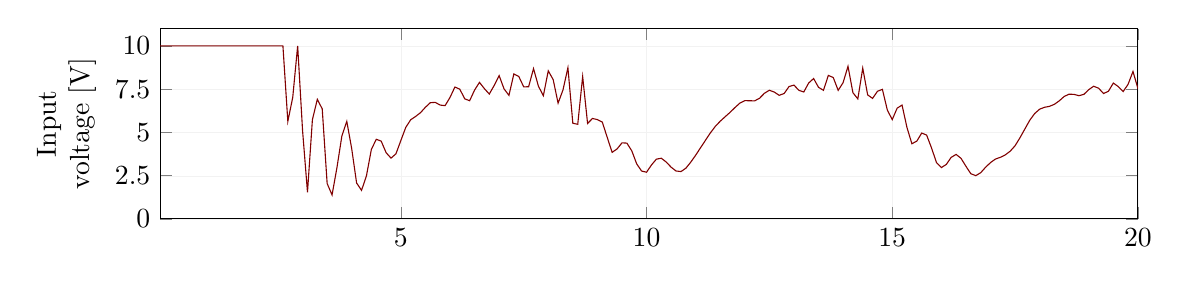
\begin{tikzpicture}
	\begin{axis}[
	ylabel style={align=center},
	ylabel= {Input\\voltage [V]},
	xmin=1, xmax=200,
	ymin=0, ymax=11,
	legend style={font=\tiny},
	grid=both,
	grid style={line width=.1pt, draw=gray!10},
	width=14cm,height=4cm,
	xticklabels={0,5,10,15,20},xtick={0,50,100,150,200},
	ytick={0,2.5,5,7.5,10},
	%thick
	]
	\addplot[color=Maroon]
	coordinates {
		(1,10)(2,10)(3,10)(4,10)(5,10)(6,10)(7,10)(8,10)(9,10)(10,10)(11,10)(12,10)(13,10)(14,10)(15,10)(16,10)(17,10)(18,10)(19,10)(20,10)(21,10)(22,10)(23,10)(24,10)(25,10)(26,10)(27,5.63302000000000)(28,7.02488000000000)(29,10)(30,5.09807000000000)(31,1.54094000000000)(32,5.73112000000000)(33,6.90821000000000)(34,6.35695000000000)(35,2.04685000000000)(36,1.38396000000000)(37,2.97249000000000)(38,4.79646000000000)(39,5.63530000000000)(40,4.05548000000000)(41,2.07109000000000)(42,1.65144000000000)(43,2.49365000000000)(44,4.01522000000000)(45,4.60064000000000)(46,4.49499000000000)(47,3.82657000000000)(48,3.51153000000000)(49,3.76052000000000)(50,4.52839000000000)(51,5.28688000000000)(52,5.72740000000000)(53,5.91875000000000)(54,6.13801000000000)(55,6.45029000000000)(56,6.71472000000000)(57,6.73331000000000)(58,6.57695000000000)(59,6.54439000000000)(60,7.01435000000000)(61,7.62055000000000)(62,7.49390000000000)(63,6.93660000000000)(64,6.82843000000000)(65,7.44093000000000)(66,7.88771000000000)(67,7.52671000000000)(68,7.21459000000000)(69,7.71304000000000)(70,8.28017000000000)(71,7.51290000000000)(72,7.13933000000000)(73,8.37620000000000)(74,8.22927000000000)(75,7.63072000000000)(76,7.63360000000000)(77,8.68319000000000)(78,7.66541000000000)(79,7.11717000000000)(80,8.55374000000000)(81,8.04907000000000)(82,6.68709000000000)(83,7.45398000000000)(84,8.73541000000000)(85,5.52574000000000)(86,5.46718000000000)(87,8.22494000000000)(88,5.51830000000000)(89,5.80265000000000)(90,5.73851000000000)(91,5.59150000000000)(92,4.70925000000000)(93,3.84629000000000)(94,4.04090000000000)(95,4.39489000000000)(96,4.37942000000000)(97,3.93170000000000)(98,3.17670000000000)(99,2.76586000000000)(100,2.69772000000000)(101,3.11556000000000)(102,3.45201000000000)(103,3.50668000000000)(104,3.28872000000000)(105,2.98944000000000)(106,2.76988000000000)(107,2.73541000000000)(108,2.92829000000000)(109,3.28035000000000)(110,3.68154000000000)(111,4.11661000000000)(112,4.54577000000000)(113,4.97236000000000)(114,5.34758000000000)(115,5.64525000000000)(116,5.90455000000000)(117,6.15690000000000)(118,6.43477000000000)(119,6.69157000000000)(120,6.83363000000000)(121,6.82615000000000)(122,6.82019000000000)(123,6.97180000000000)(124,7.26103000000000)(125,7.43317000000000)(126,7.32582000000000)(127,7.14121000000000)(128,7.24434000000000)(129,7.64737000000000)(130,7.73084000000000)(131,7.43104000000000)(132,7.33238000000000)(133,7.85272000000000)(134,8.11083000000000)(135,7.60272000000000)(136,7.42911000000000)(137,8.29078000000000)(138,8.16706000000000)(139,7.42715000000000)(140,7.87059000000000)(141,8.81561000000000)(142,7.29249000000000)(143,6.93294000000000)(144,8.71038000000000)(145,7.16527000000000)(146,6.96336000000000)(147,7.37493000000000)(148,7.48497000000000)(149,6.29337000000000)(150,5.73600000000000)(151,6.39784000000000)(152,6.57698000000000)(153,5.28062000000000)(154,4.34407000000000)(155,4.49263000000000)(156,4.96046000000000)(157,4.84445000000000)(158,4.09899000000000)(159,3.26078000000000)(160,2.96651000000000)(161,3.14659000000000)(162,3.55784000000000)(163,3.72711000000000)(164,3.50093000000000)(165,3.04214000000000)(166,2.61246000000000)(167,2.50010000000000)(168,2.66936000000000)(169,2.98517000000000)(170,3.25376000000000)(171,3.45819000000000)(172,3.55797000000000)(173,3.69672000000000)(174,3.91079000000000)(175,4.22692000000000)(176,4.69094000000000)(177,5.19951000000000)(178,5.70484000000000)(179,6.09150000000000)(180,6.34024000000000)(181,6.44887000000000)(182,6.50411000000000)(183,6.62060000000000)(184,6.82283000000000)(185,7.07519000000000)(186,7.20604000000000)(187,7.19481000000000)(188,7.11913000000000)(189,7.19503000000000)(190,7.47018000000000)(191,7.66508000000000)(192,7.55042000000000)(193,7.24535000000000)(194,7.37480000000000)(195,7.84891000000000)(196,7.64533000000000)(197,7.35766000000000)(198,7.77785000000000)(199,8.51958000000000)(200,7.53271000000000)(201,7.12168000000000)
	};
	
	\end{axis}
	\end{tikzpicture}
	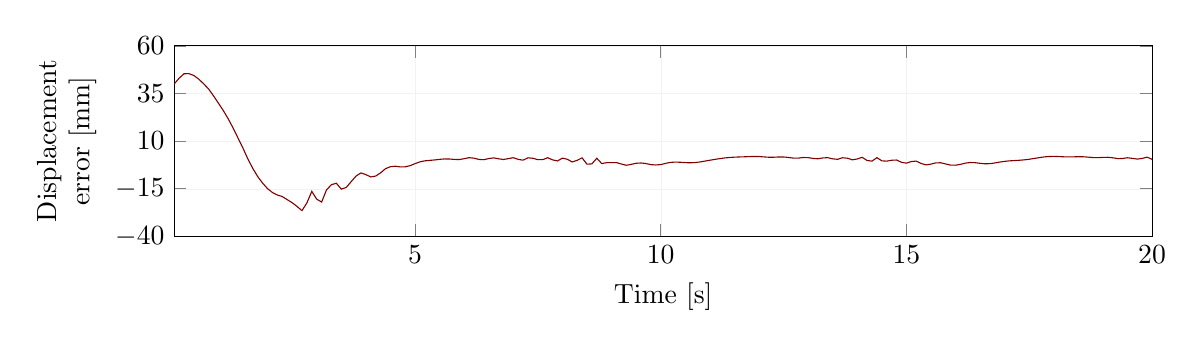
\begin{tikzpicture}
\begin{axis}[
ylabel style={align=center},
ylabel={Displacement\\error [mm]},
xlabel={Time [s]},
xmin=1, xmax=200,
ymin=-40, ymax=60,
legend style={font=\tiny},
grid=both,
grid style={line width=.1pt, draw=gray!10},
width=14cm,height=4cm,
xticklabels={0,5,10,15,20},xtick={0,50,100,150,200},
ytick={-40,-15,10,35,60},
%thick
]
\addplot[color=Maroon]
	coordinates {
	(1,40)(2,42.9750000000000)(3,45.3401000000000)(4,45.3856000000000)(5,44.4126000000000)(6,42.4828000000000)(7,40.0393000000000)(8,37.3365000000000)(9,33.7207000000000)(10,29.8298000000000)(11,25.9541000000000)(12,21.6162000000000)(13,16.7512000000000)(14,11.4867000000000)(15,6.21350000000000)(16,0.534800000000004)(17,-4.43280000000000)(18,-8.68010000000001)(19,-12.1146000000000)(20,-15.0210000000000)(21,-17.0511000000000)(22,-18.3237000000000)(23,-19.1751000000000)(24,-20.7788000000000)(25,-22.3761000000000)(26,-24.3458000000000)(27,-26.5450000000000)(28,-22.4986000000000)(29,-16.4304000000000)(30,-20.5325000000000)(31,-22.0364000000000)(32,-15.6426000000000)(33,-12.9012000000000)(34,-12.1624000000000)(35,-15.2562000000000)(36,-14.3935000000000)(37,-11.3656000000000)(38,-8.40510000000000)(39,-6.72570000000000)(40,-7.63300000000000)(41,-8.85410000000000)(42,-8.38830000000000)(43,-6.70730000000000)(44,-4.51500000000000)(45,-3.47810000000000)(46,-3.23590000000000)(47,-3.58070000000000)(48,-3.53770000000000)(49,-2.93490000000000)(50,-1.87360000000000)(51,-0.927700000000000)(52,-0.394399999999999)(53,-0.163600000000001)(54,0.0719999999999992)(55,0.377099999999999)(56,0.603800000000000)(57,0.562000000000001)(58,0.349399999999999)(59,0.281900000000000)(60,0.723700000000001)(61,1.25750000000000)(62,1.00510000000000)(63,0.347300000000004)(64,0.204400000000000)(65,0.796499999999995)(66,1.16360000000000)(67,0.686200000000007)(68,0.305499999999995)(69,0.773400000000002)(70,1.26320000000000)(71,0.369599999999998)(72,-0.0408999999999935)(73,1.20000000000000)(74,0.933099999999996)(75,0.241200000000006)(76,0.219999999999999)(77,1.24759999999999)(78,0.104999999999990)(79,-0.453699999999998)(80,1.02820000000000)(81,0.420699999999997)(82,-0.983300000000000)(83,-0.118099999999998)(84,1.17520000000000)(85,-2.15200000000000)(86,-1.99540000000000)(87,0.961900000000000)(88,-1.84090000000000)(89,-1.37250000000000)(90,-1.29940000000000)(91,-1.31640000000000)(92,-2.06700000000000)(93,-2.72329999999999)(94,-2.25640000000000)(95,-1.67670000000000)(96,-1.52450000000000)(97,-1.81980000000000)(98,-2.39280000000000)(99,-2.56440000000000)(100,-2.37610000000000)(101,-1.72060000000000)(102,-1.21210000000000)(103,-1.03620000000000)(104,-1.15060000000000)(105,-1.33480000000000)(106,-1.42090000000000)(107,-1.31330000000000)(108,-0.989099999999999)(109,-0.538100000000000)(110,-0.0831000000000000)(111,0.360299999999999)(112,0.753399999999999)(113,1.10470000000000)(114,1.36940000000000)(115,1.53010000000000)(116,1.63640000000000)(117,1.72510000000000)(118,1.83050000000000)(119,1.90420000000000)(120,1.85590000000000)(121,1.66280000000000)(122,1.49060000000000)(123,1.49310000000000)(124,1.63300000000000)(125,1.64190000000000)(126,1.37030000000000)(127,1.04870000000000)(128,1.04700000000000)(129,1.34530000000000)(130,1.29420000000000)(131,0.864999999999995)(132,0.679800000000000)(133,1.13220000000000)(134,1.27710000000000)(135,0.641300000000001)(136,0.403500000000001)(137,1.22490000000001)(138,0.978600000000000)(139,0.140900000000002)(140,0.570200000000000)(141,1.45819999999999)(142,-0.210700000000003)(143,-0.549199999999999)(144,1.28320000000001)(145,-0.390299999999996)(146,-0.553100000000001)(147,-0.0863000000000085)(148,0.0323999999999955)(149,-1.16240000000001)(150,-1.60360000000000)(151,-0.781399999999998)(152,-0.524099999999997)(153,-1.76800000000000)(154,-2.52780000000000)(155,-2.12640000000000)(156,-1.44600000000000)(157,-1.41740000000000)(158,-2.02110000000000)(159,-2.65720000000000)(160,-2.68580000000000)(161,-2.23710000000000)(162,-1.60210000000000)(163,-1.27270000000000)(164,-1.37160000000000)(165,-1.69320000000000)(166,-1.95360000000000)(167,-1.87060000000000)(168,-1.51430000000000)(169,-1.04700000000000)(170,-0.673700000000000)(171,-0.401900000000001)(172,-0.262000000000000)(173,-0.0969999999999995)(174,0.126799999999999)(175,0.430200000000001)(176,0.851199999999999)(177,1.27470000000000)(178,1.65250000000000)(179,1.87390000000000)(180,1.93530000000000)(181,1.85040000000000)(182,1.72060000000000)(183,1.66500000000000)(184,1.70070000000000)(185,1.78300000000000)(186,1.73560000000000)(187,1.55080000000000)(188,1.32000000000000)(189,1.26390000000000)(190,1.41270000000000)(191,1.46630000000000)(192,1.20500000000001)(193,0.779399999999995)(194,0.831000000000003)(195,1.22200000000000)(196,0.896200000000000)(197,0.518900000000002)(198,0.887200000000000)(199,1.54020000000001)(200,0.399300000000011)
	};
	
\end{axis}
\end{tikzpicture}	
	\caption{Displacement control, 7 kilograms, 1 $\nicefrac{rad}{s}$}
	\label{fig:7kg-1rad}
\end{figure}


\begin{figure}[H]
	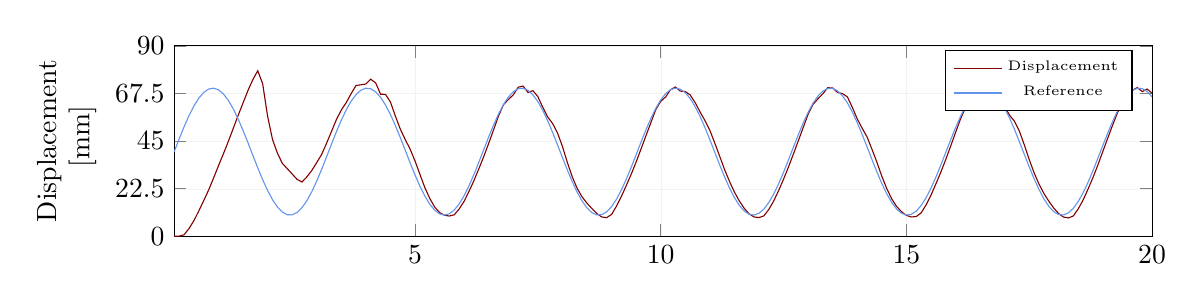
\begin{tikzpicture}
	\begin{axis}[
	ylabel style={align=center},
	ylabel={Displacement\\~[mm]},
	xmin=1, xmax=200,
	ymin=0, ymax=90,
	legend style={font=\tiny},
	grid=both,
	grid style={line width=.1pt, draw=gray!10},
	width=14cm,height=4cm,
	xticklabels={0,5,10,15,20},xtick={0,50,100,150,200},
	ytick={0,22.5,45,67.5,90},
	%thick
	]
	
	\addplot[
	color=Maroon
	]
	coordinates {
(1,0)(2,0.0400000000000000)(3,0.700000000000000)(4,3.62000000000000)(5,7.34000000000000)(6,11.9600000000000)(7,16.8300000000000)(8,21.8200000000000)(9,27.4700000000000)(10,33.3000000000000)(11,38.9200000000000)(12,44.7500000000000)(13,50.8900000000000)(14,57.0500000000000)(15,62.9400000000000)(16,68.8600000000000)(17,74.0300000000000)(18,78.2100000000000)(19,72.0900000000000)(20,56.7500000000000)(21,45.7700000000000)(22,39.3200000000000)(23,34.4600000000000)(24,31.9500000000000)(25,29.4300000000000)(26,26.8900000000000)(27,25.6200000000000)(28,28.0700000000000)(29,31.0800000000000)(30,34.8300000000000)(31,38.6500000000000)(32,43.9400000000000)(33,49.5100000000000)(34,55.1200000000000)(35,59.6300000000000)(36,63.1500000000000)(37,67.3800000000000)(38,71.2400000000000)(39,71.5800000000000)(40,71.9400000000000)(41,74.2200000000000)(42,72.4500000000000)(43,67.1300000000000)(44,67.0500000000000)(45,63.4500000000000)(46,56.8200000000000)(47,50.7200000000000)(48,45.7600000000000)(49,41.2100000000000)(50,35.6000000000000)(51,29.3100000000000)(52,23.0300000000000)(53,17.9100000000000)(54,13.8000000000000)(55,11.2200000000000)(56,9.90000000000000)(57,9.56000000000000)(58,10.1600000000000)(59,12.9400000000000)(60,16.5300000000000)(61,21.2300000000000)(62,26.3500000000000)(63,31.9200000000000)(64,37.6900000000000)(65,43.9300000000000)(66,50.3600000000000)(67,56.8400000000000)(68,62.1700000000000)(69,64.6300000000000)(70,66.8200000000000)(71,70.4300000000000)(72,70.9500000000000)(73,67.9400000000000)(74,68.7900000000000)(75,66.0200000000000)(76,60.9800000000000)(77,56.3600000000000)(78,53.3000000000000)(79,48.8200000000000)(80,42.5000000000000)(81,34.9300000000000)(82,28.1000000000000)(83,22.6700000000000)(84,18.6300000000000)(85,15.6300000000000)(86,13.0900000000000)(87,10.7600000000000)(88,9.13000000000000)(89,8.78000000000000)(90,10.3000000000000)(91,14.1900000000000)(92,18.8100000000000)(93,23.9600000000000)(94,29.3000000000000)(95,35.0500000000000)(96,41.2400000000000)(97,47.4800000000000)(98,53.6900000000000)(99,59.8500000000000)(100,63.7400000000000)(101,65.8100000000000)(102,69.2500000000000)(103,70.5500000000000)(104,68.5900000000000)(105,68.3900000000000)(106,66.7900000000000)(107,63.2300000000000)(108,58.7900000000000)(109,54.7500000000000)(110,50.0800000000000)(111,44.1200000000000)(112,37.8400000000000)(113,31.5700000000000)(114,25.9200000000000)(115,20.9400000000000)(116,16.6900000000000)(117,13.2000000000000)(118,10.5700000000000)(119,9.12000000000000)(120,8.82000000000000)(121,9.63000000000000)(122,12.6500000000000)(123,16.6400000000000)(124,21.5800000000000)(125,26.9400000000000)(126,32.6900000000000)(127,38.7900000000000)(128,45.0500000000000)(129,51.3500000000000)(130,57.6500000000000)(131,62.3100000000000)(132,64.9500000000000)(133,67.3400000000000)(134,70.1900000000000)(135,70.0900000000000)(136,67.9600000000000)(137,67.4200000000000)(138,65.8300000000000)(139,60.9400000000000)(140,55.4700000000000)(141,51.0600000000000)(142,46.9200000000000)(143,41.0800000000000)(144,35)(145,28.3600000000000)(146,22.5900000000000)(147,17.7400000000000)(148,14.1300000000000)(149,11.5900000000000)(150,9.88000000000000)(151,9.12000000000000)(152,9.31000000000000)(153,11.0200000000000)(154,14.7900000000000)(155,19.3700000000000)(156,24.7000000000000)(157,30.2100000000000)(158,36.1800000000000)(159,42.5000000000000)(160,48.9800000000000)(161,55.3200000000000)(162,60.6600000000000)(163,63.5200000000000)(164,66.3500000000000)(165,69.9700000000000)(166,70.2000000000000)(167,67.8500000000000)(168,69.6200000000000)(169,67.5000000000000)(170,61.2300000000000)(171,57.2300000000000)(172,54.3300000000000)(173,49.6500000000000)(174,43.2000000000000)(175,36.2600000000000)(176,29.9400000000000)(177,24.6100000000000)(178,20.1700000000000)(179,16.5100000000000)(180,13.3200000000000)(181,10.6800000000000)(182,9.06000000000000)(183,8.66000000000000)(184,9.63000000000000)(185,13.0500000000000)(186,17.2700000000000)(187,22.4500000000000)(188,27.8900000000000)(189,33.8600000000000)(190,40.2000000000000)(191,46.4800000000000)(192,52.6700000000000)(193,58.5800000000000)(194,62.5500000000000)(195,64.8900000000000)(196,69.0100000000000)(197,70.2700000000000)(198,68.3600000000000)(199,69.5700000000000)(200,67.5500000000000)
	};
	
	\addplot[color=CornflowerBlue]
	coordinates {
(1,40)(2,45.9601000000000)(3,51.6826000000000)(4,56.9393000000000)(5,61.5207000000000)(6,65.2441000000000)(7,67.9612000000000)(8,69.5635000000000)(9,69.9872000000000)(10,69.2154000000000)(11,67.2789000000000)(12,64.2549000000000)(13,60.2639000000000)(14,55.4650000000000)(15,50.0496000000000)(16,44.2336000000000)(17,38.2488000000000)(18,32.3338000000000)(19,26.7244000000000)(20,21.6443000000000)(21,17.2959000000000)(22,13.8527000000000)(23,11.4519000000000)(24,10.1893000000000)(25,10.1151000000000)(26,11.2323000000000)(27,13.4964000000000)(28,16.8171000000000)(29,21.0620000000000)(30,26.0619000000000)(31,31.6175000000000)(32,37.5073000000000)(33,43.4965000000000)(34,49.3462000000000)(35,54.8234000000000)(36,59.7096000000000)(37,63.8100000000000)(38,66.9612000000000)(39,69.0376000000000)(40,69.9563000000000)(41,69.6807000000000)(42,68.2219000000000)(43,65.6380000000000)(44,62.0319000000000)(45,57.5475000000000)(46,52.3636000000000)(47,46.6867000000000)(48,40.7433000000000)(49,34.7702000000000)(50,29.0056000000000)(51,23.6794000000000)(52,19.0038000000000)(53,15.1652000000000)(54,12.3167000000000)(55,10.5719000000000)(56,10.0003000000000)(57,10.6247000000000)(58,12.4201000000000)(59,15.3151000000000)(60,19.1942000000000)(61,23.9028000000000)(62,29.2531000000000)(63,35.0319000000000)(64,41.0087000000000)(65,46.9453000000000)(66,52.6050000000000)(67,57.7622000000000)(68,62.2113000000000)(69,65.7749000000000)(70,68.3109000000000)(71,69.7182000000000)(72,69.9408000000000)(73,68.9697000000000)(74,66.8437000000000)(75,63.6476000000000)(76,59.5086000000000)(77,54.5920000000000)(78,49.0936000000000)(79,43.2326000000000)(80,37.2428000000000)(81,31.3629000000000)(82,25.8273000000000)(83,20.8568000000000)(84,16.6494000000000)(85,13.3730000000000)(86,11.1581000000000)(87,10.0930000000000)(88,10.2202000000000)(89,11.5347000000000)(90,13.9839000000000)(91,17.4704000000000)(92,21.8550000000000)(93,26.9630000000000)(94,32.5908000000000)(95,38.5139000000000)(96,44.4963000000000)(97,50.2994000000000)(98,55.6920000000000)(99,60.4589000000000)(100,64.4102000000000)(101,67.3884000000000)(102,69.2746000000000)(103,69.9938000000000)(104,69.5172000000000)(105,67.8639000000000)(106,65.0997000000000)(107,61.3348000000000)(108,56.7195000000000)(109,51.4375000000000)(110,45.6996000000000)(111,39.7345000000000)(112,33.7799000000000)(113,28.0733000000000)(114,22.8422000000000)(115,18.2952000000000)(116,14.6134000000000)(117,11.9437000000000)(118,10.3925000000000)(119,10.0217000000000)(120,10.8460000000000)(121,12.8326000000000)(122,15.9023000000000)(123,19.9327000000000)(124,24.7631000000000)(125,30.2009000000000)(126,36.0294000000000)(127,42.0162000000000)(128,47.9227000000000)(129,53.5132000000000)(130,58.5651000000000)(131,62.8768000000000)(132,66.2764000000000)(133,68.6286000000000)(134,69.8393000000000)(135,69.8605000000000)(136,68.6913000000000)(137,66.3782000000000)(138,63.0135000000000)(139,58.7313000000000)(140,53.7024000000000)(141,48.1272000000000)(142,42.2280000000000)(143,36.2399000000000)(144,30.4018000000000)(145,24.9463000000000)(146,20.0910000000000)(147,16.0294000000000)(148,12.9234000000000)(149,10.8968000000000)(150,10.0305000000000)(151,10.3591000000000)(152,11.8692000000000)(153,14.5009000000000)(154,18.1492000000000)(155,22.6685000000000)(156,27.8789000000000)(157,33.5724000000000)(158,39.5222000000000)(159,45.4911000000000)(160,51.2410000000000)(161,56.5428000000000)(162,61.1851000000000)(163,64.9828000000000)(164,67.7845000000000)(165,69.4785000000000)(166,69.9974000000000)(167,69.3203000000000)(168,67.4743000000000)(169,64.5330000000000)(170,60.6136000000000)(171,55.8725000000000)(172,50.4985000000000)(173,44.7061000000000)(174,38.7260000000000)(175,32.7967000000000)(176,27.1545000000000)(177,22.0245000000000)(178,17.6111000000000)(179,14.0903000000000)(180,11.6024000000000)(181,10.2466000000000)(182,10.0770000000000)(183,11.1004000000000)(184,13.2759000000000)(185,16.5168000000000)(186,20.6939000000000)(187,25.6406000000000)(188,31.1599000000000)(189,37.0315000000000)(190,43.0215000000000)(191,48.8911000000000)(192,54.4061000000000)(193,59.3469000000000)(194,63.5164000000000)(195,66.7483000000000)(196,68.9139000000000)(197,69.9267000000000)(198,69.7465000000000)(199,68.3804000000000)(200,65.8828000000000)
	};
	
	\addlegendentry{Displacement}
	\addlegendentry{Reference}
	
	\end{axis}
	
	\end{tikzpicture}
	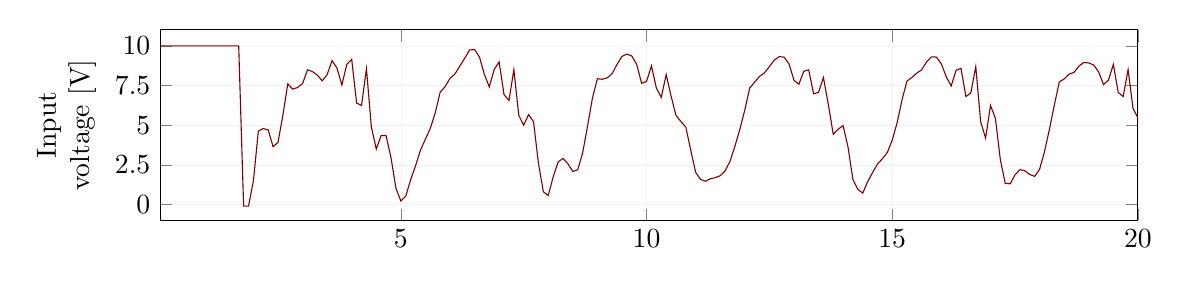
\begin{tikzpicture}
	\begin{axis}[
	ylabel style={align=center},
	ylabel= {Input\\voltage [V]},
	xmin=1, xmax=200,
	ymin=-1, ymax=11,
	legend style={font=\tiny},
	grid=both,
	grid style={line width=.1pt, draw=gray!10},
	width=14cm,height=4cm,
	xticklabels={0,5,10,15,20},xtick={0,50,100,150,200},
	ytick={0,2.5,5,7.5,10},
	%thick
	]
	\addplot[color=Maroon]
	coordinates {
(1,10)(2,10)(3,10)(4,10)(5,10)(6,10)(7,10)(8,10)(9,10)(10,10)(11,10)(12,10)(13,10)(14,10)(15,10)(16,10)(17,10)(18,-0.100000000000000)(19,-0.100000000000000)(20,1.50496000000000)(21,4.62605000000000)(22,4.78544000000000)(23,4.69792000000000)(24,3.64445000000000)(25,3.91417000000000)(26,5.63988000000000)(27,7.60820000000000)(28,7.26654000000000)(29,7.37618000000000)(30,7.62432000000000)(31,8.48311000000000)(32,8.37965000000000)(33,8.15554000000000)(34,7.79395000000000)(35,8.18373000000000)(36,9.06927000000000)(37,8.59567000000000)(38,7.52988000000000)(39,8.83835000000000)(40,9.14282000000000)(41,6.38890000000000)(42,6.24614000000000)(43,8.55938000000000)(44,4.88413000000000)(45,3.49792000000000)(46,4.35371000000000)(47,4.33121000000000)(48,2.94444000000000)(49,1.01970000000000)(50,0.221153000000000)(51,0.525456000000000)(52,1.56679000000000)(53,2.44561000000000)(54,3.43266000000000)(55,4.11951000000000)(56,4.80308000000000)(57,5.77749000000000)(58,7.07943000000000)(59,7.42044000000000)(60,7.94706000000000)(61,8.22205000000000)(62,8.71964000000000)(63,9.21871000000000)(64,9.73671000000000)(65,9.76518000000000)(66,9.29643000000000)(67,8.19812000000000)(68,7.40942000000000)(69,8.51712000000000)(70,8.97762000000000)(71,6.92406000000000)(72,6.55546000000000)(73,8.49347000000000)(74,5.62045000000000)(75,4.99965000000000)(76,5.66348000000000)(77,5.21967000000000)(78,2.60445000000000)(79,0.802868000000000)(80,0.574314000000000)(81,1.73870000000000)(82,2.67643000000000)(83,2.90862000000000)(84,2.55994000000000)(85,2.08544000000000)(86,2.18482000000000)(87,3.25655000000000)(88,4.94707000000000)(89,6.72054000000000)(90,7.92528000000000)(91,7.89012000000000)(92,7.98279000000000)(93,8.24531000000000)(94,8.83337000000000)(95,9.33559000000000)(96,9.47437000000000)(97,9.36313000000000)(98,8.82760000000000)(99,7.63473000000000)(100,7.75693000000000)(101,8.73209000000000)(102,7.33619000000000)(103,6.75782000000000)(104,8.18561000000000)(105,6.82499000000000)(106,5.60819000000000)(107,5.23432000000000)(108,4.86942000000000)(109,3.42043000000000)(110,2.02126000000000)(111,1.57809000000000)(112,1.46498000000000)(113,1.62239000000000)(114,1.69162000000000)(115,1.81677000000000)(116,2.12052000000000)(117,2.73317000000000)(118,3.68638000000000)(119,4.74782000000000)(120,5.96231000000000)(121,7.34152000000000)(122,7.71147000000000)(123,8.07708000000000)(124,8.29674000000000)(125,8.69290000000000)(126,9.09749000000000)(127,9.31823000000000)(128,9.28727000000000)(129,8.86510000000000)(130,7.83325000000000)(131,7.57646000000000)(132,8.39281000000000)(133,8.48758000000000)(134,6.97722000000000)(135,7.06335000000000)(136,8.00115000000000)(137,6.30119000000000)(138,4.42231000000000)(139,4.74848000000000)(140,4.96867000000000)(141,3.62671000000000)(142,1.57421000000000)(143,0.956978000000000)(144,0.714842000000000)(145,1.43954000000000)(146,2.01284000000000)(147,2.55131000000000)(148,2.88425000000000)(149,3.27705000000000)(150,4.05145000000000)(151,5.15501000000000)(152,6.59911000000000)(153,7.77672000000000)(154,8.00306000000000)(155,8.27835000000000)(156,8.48853000000000)(157,8.98997000000000)(158,9.30601000000000)(159,9.28908000000000)(160,8.85812000000000)(161,8.04602000000000)(162,7.47058000000000)(163,8.46079000000000)(164,8.57878000000000)(165,6.79627000000000)(166,7.03594000000000)(167,8.68860000000000)(168,5.21964000000000)(169,4.18377000000000)(170,6.23771000000000)(171,5.43492000000000)(172,2.82523000000000)(173,1.32960000000000)(174,1.30511000000000)(175,1.86840000000000)(176,2.19993000000000)(177,2.12136000000000)(178,1.88941000000000)(179,1.77270000000000)(180,2.23284000000000)(181,3.34532000000000)(182,4.75240000000000)(183,6.27745000000000)(184,7.72697000000000)(185,7.91245000000000)(186,8.21622000000000)(187,8.32537000000000)(188,8.72366000000000)(189,8.95230000000000)(190,8.91946000000000)(191,8.79115000000000)(192,8.35734000000000)(193,7.56172000000000)(194,7.83787000000000)(195,8.82644000000000)(196,7.05783000000000)(197,6.80108000000000)(198,8.49653000000000)(199,6.05906000000000)(200,5.46254000000000)
	};
	
	\end{axis}
	\end{tikzpicture}
	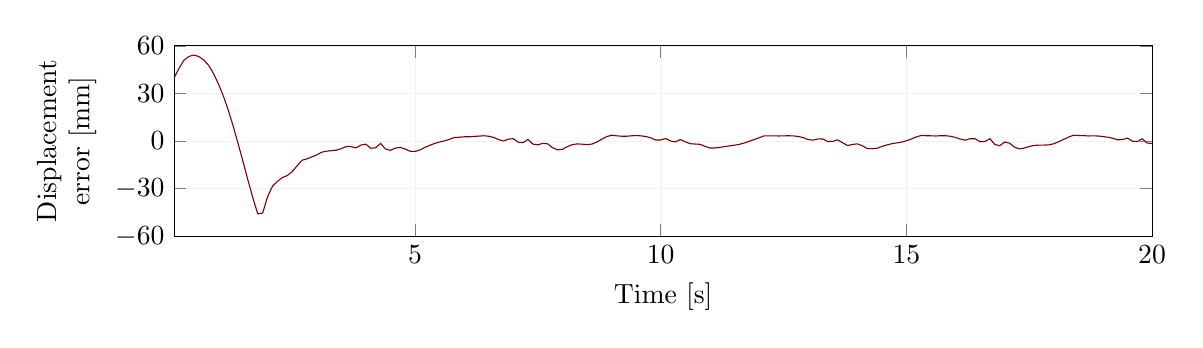
\begin{tikzpicture}
	\begin{axis}[
	ylabel style={align=center},
	ylabel={Displacement\\error [mm]},
	xlabel={Time [s]},
	xmin=1, xmax=200,
	ymin=-60, ymax=60,
	legend style={font=\tiny},
	grid=both,
	grid style={line width=.1pt, draw=gray!10},
	width=14cm,height=4cm,
	xticklabels={0,5,10,15,20},xtick={0,50,100,150,200},
	ytick={-60,-30,0,30,60},
	%thick
	]
	\addplot[color=Maroon]
	coordinates {
(1,40)(2,45.9201000000000)(3,50.9826000000000)(4,53.3193000000000)(5,54.1807000000000)(6,53.2841000000000)(7,51.1312000000000)(8,47.7435000000000)(9,42.5172000000000)(10,35.9154000000000)(11,28.3589000000000)(12,19.5049000000000)(13,9.37390000000000)(14,-1.58499999999999)(15,-12.8904000000000)(16,-24.6264000000000)(17,-35.7812000000000)(18,-45.8762000000000)(19,-45.3656000000000)(20,-35.1057000000000)(21,-28.4741000000000)(22,-25.4673000000000)(23,-23.0081000000000)(24,-21.7607000000000)(25,-19.3149000000000)(26,-15.6577000000000)(27,-12.1236000000000)(28,-11.2529000000000)(29,-10.0180000000000)(30,-8.76810000000000)(31,-7.03250000000000)(32,-6.43270000000000)(33,-6.01350000000000)(34,-5.77379999999999)(35,-4.80660000000000)(36,-3.44040000000000)(37,-3.56999999999999)(38,-4.27879999999999)(39,-2.54240000000000)(40,-1.98370000000000)(41,-4.53930000000000)(42,-4.22810000000000)(43,-1.49199999999999)(44,-5.01810000000000)(45,-5.90250000000000)(46,-4.45640000000000)(47,-4.03330000000000)(48,-5.01670000000000)(49,-6.43980000000000)(50,-6.59440000000000)(51,-5.63060000000000)(52,-4.02620000000000)(53,-2.74480000000000)(54,-1.48330000000000)(55,-0.648100000000001)(56,0.100299999999999)(57,1.06470000000000)(58,2.26010000000000)(59,2.37510000000000)(60,2.66420000000000)(61,2.67280000000000)(62,2.90310000000000)(63,3.11190000000000)(64,3.31870000000000)(65,3.01530000000000)(66,2.24500000000000)(67,0.922199999999997)(68,0.0412999999999997)(69,1.14490000000001)(70,1.49090000000001)(71,-0.711800000000011)(72,-1.00920000000001)(73,1.02970000000001)(74,-1.94630000000001)(75,-2.37240000000000)(76,-1.47140000000000)(77,-1.76800000000000)(78,-4.20640000000000)(79,-5.58740000000000)(80,-5.25720000000000)(81,-3.56710000000000)(82,-2.27270000000000)(83,-1.81320000000000)(84,-1.98060000000000)(85,-2.25700000000000)(86,-1.93190000000000)(87,-0.667000000000000)(88,1.09020000000000)(89,2.75470000000000)(90,3.68390000000000)(91,3.28040000000000)(92,3.04500000000000)(93,3.00300000000000)(94,3.29080000000000)(95,3.46390000000000)(96,3.25630000000000)(97,2.81940000000000)(98,2.00200000000000)(99,0.608899999999998)(100,0.670200000000001)(101,1.57840000000000)(102,0.0246000000000066)(103,-0.556200000000004)(104,0.927199999999999)(105,-0.526100000000000)(106,-1.69030000000001)(107,-1.89520000000000)(108,-2.07050000000000)(109,-3.31250000000000)(110,-4.38040000000000)(111,-4.38550000000000)(112,-4.06010000000001)(113,-3.49670000000000)(114,-3.07780000000000)(115,-2.64480000000000)(116,-2.07660000000000)(117,-1.25630000000000)(118,-0.177500000000000)(119,0.901700000000000)(120,2.02600000000000)(121,3.20260000000000)(122,3.25230000000000)(123,3.29270000000000)(124,3.18310000000000)(125,3.26090000000000)(126,3.33940000000001)(127,3.22620000000000)(128,2.87270000000000)(129,2.16320000000000)(130,0.915100000000003)(131,0.566800000000001)(132,1.32639999999999)(133,1.28860000000000)(134,-0.350700000000003)(135,-0.229500000000002)(136,0.731300000000005)(137,-1.04180000000000)(138,-2.81650000000000)(139,-2.20870000000000)(140,-1.76760000000000)(141,-2.93280000000000)(142,-4.69200000000000)(143,-4.84010000000000)(144,-4.59820000000000)(145,-3.41370000000000)(146,-2.49900000000000)(147,-1.71060000000000)(148,-1.20660000000000)(149,-0.693199999999999)(150,0.150499999999999)(151,1.23910000000000)(152,2.55920000000000)(153,3.48090000000000)(154,3.35920000000000)(155,3.29850000000000)(156,3.17890000000000)(157,3.36240000000000)(158,3.34220000000000)(159,2.99110000000000)(160,2.26100000000000)(161,1.22280000000000)(162,0.525100000000002)(163,1.46279999999999)(164,1.43450000000000)(165,-0.491500000000002)(166,-0.202600000000004)(167,1.47030000000001)(168,-2.14570000000001)(169,-2.96700000000000)(170,-0.616399999999999)(171,-1.35749999999999)(172,-3.83150000000000)(173,-4.94390000000000)(174,-4.47400000000000)(175,-3.46330000000000)(176,-2.78550000000000)(177,-2.58550000000000)(178,-2.55890000000000)(179,-2.41970000000000)(180,-1.71760000000000)(181,-0.433399999999999)(182,1.01700000000000)(183,2.44040000000000)(184,3.64590000000000)(185,3.46680000000000)(186,3.42390000000000)(187,3.19060000000000)(188,3.26990000000000)(189,3.17150000000000)(190,2.82150000000000)(191,2.41110000000000)(192,1.73610000000000)(193,0.766900000000000)(194,0.966400000000000)(195,1.85830000000000)(196,-0.0961000000000070)(197,-0.343299999999999)(198,1.38650000000000)(199,-1.18960000000000)(200,-1.66719999999999)
	};
	\end{axis}
	\end{tikzpicture}	
	\caption{Displacement control, 7 kilograms, 2 $\nicefrac{rad}{s}$}
	\label{fig:7kg-2rad}
\end{figure}

\begin{figure}[H]
	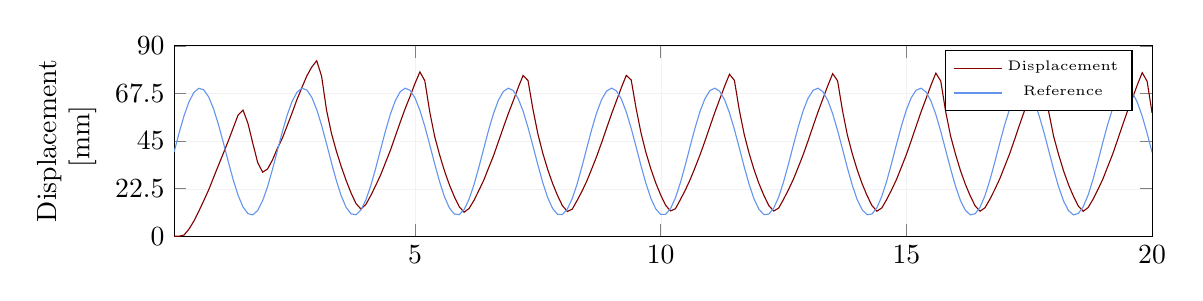
\begin{tikzpicture}
	\begin{axis}[
	ylabel style={align=center},
	ylabel={Displacement\\~[mm]},
	xmin=1, xmax=200,
	ymin=0, ymax=90,
	legend style={font=\tiny},
	grid=both,
	grid style={line width=.1pt, draw=gray!10},
	width=14cm,height=4cm,
	xticklabels={0,5,10,15,20},xtick={0,50,100,150,200},
	ytick={0,22.5,45,67.5,90},
	%thick
	]
	
	\addplot[
	color=Maroon
	]
	coordinates {
(1,0)(2,0.0200000000000000)(3,0.570000000000000)(4,3.36000000000000)(5,7.15000000000000)(6,11.7900000000000)(7,16.7700000000000)(8,21.8600000000000)(9,27.6900000000000)(10,33.5200000000000)(11,39.1900000000000)(12,45.0100000000000)(13,51.1300000000000)(14,57.3000000000000)(15,59.5800000000000)(16,53.4100000000000)(17,43.8600000000000)(18,34.7400000000000)(19,30.2700000000000)(20,31.8000000000000)(21,36.0600000000000)(22,41.5700000000000)(23,46.2800000000000)(24,52.3200000000000)(25,58.3200000000000)(26,64.7600000000000)(27,70.3600000000000)(28,75.8300000000000)(29,79.9900000000000)(30,82.9600000000000)(31,75.5500000000000)(32,59.5600000000000)(33,48.6300000000000)(34,40.2400000000000)(35,32.8700000000000)(36,26.3000000000000)(37,20.3800000000000)(38,15.4400000000000)(39,12.8500000000000)(40,15.0300000000000)(41,19.2300000000000)(42,23.9700000000000)(43,28.9400000000000)(44,34.8300000000000)(45,40.6400000000000)(46,47.3300000000000)(47,53.9200000000000)(48,60.3300000000000)(49,66.0800000000000)(50,72.2400000000000)(51,77.6700000000000)(52,73.4800000000000)(53,58.8200000000000)(54,47.2000000000000)(55,38.5300000000000)(56,30.8700000000000)(57,24.3100000000000)(58,18.7400000000000)(59,13.9700000000000)(60,11.3600000000000)(61,13.1100000000000)(62,16.9600000000000)(63,21.6400000000000)(64,26.5500000000000)(65,32.4100000000000)(66,38.2200000000000)(67,44.8500000000000)(68,51.5200000000000)(69,58.0300000000000)(70,64.0200000000000)(71,70.2600000000000)(72,75.9900000000000)(73,73.5900000000000)(74,60.0700000000000)(75,48.4600000000000)(76,39.3000000000000)(77,31.6300000000000)(78,24.9800000000000)(79,19.2900000000000)(80,14.4700000000000)(81,11.7100000000000)(82,12.8000000000000)(83,16.9300000000000)(84,21.3500000000000)(85,26.2800000000000)(86,32.0100000000000)(87,37.8900000000000)(88,44.3800000000000)(89,51.1300000000000)(90,57.8000000000000)(91,64.0400000000000)(92,70.2500000000000)(93,76.0400000000000)(94,73.8700000000000)(95,60.3800000000000)(96,48.7900000000000)(97,39.5400000000000)(98,31.8300000000000)(99,25.1800000000000)(100,19.5000000000000)(101,14.6500000000000)(102,11.9600000000000)(103,13)(104,17.2800000000000)(105,21.7700000000000)(106,26.7700000000000)(107,32.4800000000000)(108,38.4200000000000)(109,44.9100000000000)(110,51.7100000000000)(111,58.4200000000000)(112,64.6800000000000)(113,70.8400000000000)(114,76.5600000000000)(115,73.6700000000000)(116,59.6500000000000)(117,48.1300000000000)(118,39.1600000000000)(119,31.4900000000000)(120,24.9100000000000)(121,19.3200000000000)(122,14.5300000000000)(123,11.9300000000000)(124,13.2700000000000)(125,17.4300000000000)(126,21.9700000000000)(127,26.9000000000000)(128,32.6400000000000)(129,38.5500000000000)(130,45.1200000000000)(131,51.9700000000000)(132,58.6500000000000)(133,64.8900000000000)(134,71.1000000000000)(135,76.8300000000000)(136,73.5000000000000)(137,59.4100000000000)(138,47.7700000000000)(139,38.9700000000000)(140,31.3300000000000)(141,24.8000000000000)(142,19.2400000000000)(143,14.4900000000000)(144,11.8600000000000)(145,13.3900000000000)(146,17.3800000000000)(147,21.9600000000000)(148,26.8900000000000)(149,32.7200000000000)(150,38.6100000000000)(151,45.2600000000000)(152,52.1100000000000)(153,58.8300000000000)(154,65.0500000000000)(155,71.3300000000000)(156,77.0900000000000)(157,73.3400000000000)(158,58.8900000000000)(159,47.3500000000000)(160,38.7300000000000)(161,31.1000000000000)(162,24.6000000000000)(163,19.0700000000000)(164,14.3500000000000)(165,11.8300000000000)(166,13.4800000000000)(167,17.5100000000000)(168,22.1600000000000)(169,27.1100000000000)(170,33)(171,38.8600000000000)(172,45.5700000000000)(173,52.4300000000000)(174,59.1000000000000)(175,65.2400000000000)(176,71.5400000000000)(177,77.3000000000000)(178,73.2100000000000)(179,58.4100000000000)(180,46.9100000000000)(181,38.4600000000000)(182,30.8300000000000)(183,24.3600000000000)(184,18.9100000000000)(185,14.2300000000000)(186,11.8100000000000)(187,13.5900000000000)(188,17.5000000000000)(189,22.1400000000000)(190,27.0900000000000)(191,33.0300000000000)(192,38.9000000000000)(193,45.6600000000000)(194,52.5200000000000)(195,59.1500000000000)(196,65.2300000000000)(197,71.5400000000000)(198,77.3100000000000)(199,73.2000000000000)(200,58.2800000000000)
	};
	
	\addplot[color=CornflowerBlue]
	coordinates {
(1,40)(2,48.8656000000000)(3,56.9393000000000)(4,63.4998000000000)(5,67.9612000000000)(6,69.9248000000000)(7,69.2154000000000)(8,65.8963000000000)(9,60.2639000000000)(10,52.8214000000000)(11,44.2336000000000)(12,35.2676000000000)(13,26.7244000000000)(14,19.3670000000000)(15,13.8527000000000)(16,10.6741000000000)(17,10.1151000000000)(18,12.2256000000000)(19,16.8171000000000)(20,23.4794000000000)(21,31.6175000000000)(22,40.5044000000000)(23,49.3462000000000)(24,57.3532000000000)(25,63.8100000000000)(26,68.1400000000000)(27,69.9563000000000)(28,69.0967000000000)(29,65.6380000000000)(30,59.8891000000000)(31,52.3636000000000)(32,43.7336000000000)(33,34.7702000000000)(34,26.2739000000000)(35,19.0038000000000)(36,13.6091000000000)(37,10.5719000000000)(38,10.1634000000000)(39,12.4201000000000)(40,17.1405000000000)(41,23.9028000000000)(42,32.1030000000000)(43,41.0087000000000)(44,49.8242000000000)(45,57.7622000000000)(46,64.1135000000000)(47,68.3109000000000)(48,69.9793000000000)(49,68.9697000000000)(50,65.3724000000000)(51,59.5086000000000)(52,51.9022000000000)(53,43.2326000000000)(54,34.2742000000000)(55,25.8273000000000)(56,18.6464000000000)(57,13.3730000000000)(58,10.4780000000000)(59,10.2202000000000)(60,12.6225000000000)(61,17.4704000000000)(62,24.3307000000000)(63,32.5908000000000)(64,41.5127000000000)(65,50.2994000000000)(66,58.1662000000000)(67,64.4102000000000)(68,68.4737000000000)(69,69.9938000000000)(70,68.8346000000000)(71,65.0997000000000)(72,59.1227000000000)(73,51.4375000000000)(74,42.7307000000000)(75,33.7799000000000)(76,25.3848000000000)(77,18.2952000000000)(78,13.1444000000000)(79,10.3925000000000)(80,10.2854000000000)(81,12.8326000000000)(82,17.8066000000000)(83,24.7631000000000)(84,33.0806000000000)(85,42.0162000000000)(86,50.7718000000000)(87,58.5651000000000)(88,64.7000000000000)(89,68.6286000000000)(90,69.9998000000000)(91,68.6913000000000)(92,64.8198000000000)(93,58.7313000000000)(94,50.9696000000000)(95,42.2280000000000)(96,33.2873000000000)(97,24.9463000000000)(98,17.9500000000000)(99,12.9234000000000)(100,10.3154000000000)(101,10.3591000000000)(102,13.0505000000000)(103,18.1492000000000)(104,25.1998000000000)(105,33.5724000000000)(106,42.5192000000000)(107,51.2410000000000)(108,58.9587000000000)(109,64.9828000000000)(110,68.7753000000000)(111,69.9974000000000)(112,68.5399000000000)(113,64.5330000000000)(114,58.3347000000000)(115,50.4985000000000)(116,41.7246000000000)(117,32.7967000000000)(118,24.5121000000000)(119,17.6111000000000)(120,12.7100000000000)(121,10.2466000000000)(122,10.4410000000000)(123,13.2759000000000)(124,18.4979000000000)(125,25.6406000000000)(126,34.0660000000000)(127,43.0215000000000)(128,51.7071000000000)(129,59.3469000000000)(130,65.2585000000000)(131,68.9139000000000)(132,69.9864000000000)(133,68.3804000000000)(134,64.2392000000000)(135,57.9328000000000)(136,50.0245000000000)(137,41.2208000000000)(138,32.3080000000000)(139,24.0823000000000)(140,17.2785000000000)(141,12.5044000000000)(142,10.1863000000000)(143,10.5314000000000)(144,13.5089000000000)(145,18.8527000000000)(146,26.0855000000000)(147,34.5613000000000)(148,43.5229000000000)(149,52.1699000000000)(150,59.7297000000000)(151,65.5271000000000)(152,69.0443000000000)(153,69.9670000000000)(154,68.2129000000000)(155,63.9386000000000)(156,57.5259000000000)(157,49.5477000000000)(158,40.7166000000000)(159,31.8215000000000)(160,23.6570000000000)(161,16.9524000000000)(162,12.3065000000000)(163,10.1344000000000)(164,10.6301000000000)(165,13.7493000000000)(166,19.2135000000000)(167,26.5344000000000)(168,35.0582000000000)(169,44.0234000000000)(170,52.6292000000000)(171,60.1069000000000)(172,65.7885000000000)(173,69.1665000000000)(174,69.9391000000000)(175,68.0374000000000)(176,63.6312000000000)(177,57.1140000000000)(178,49.0682000000000)(179,40.2123000000000)(180,31.3374000000000)(181,23.2363000000000)(182,16.6327000000000)(183,12.1164000000000)(184,10.0909000000000)(185,10.7371000000000)(186,13.9972000000000)(187,19.5801000000000)(188,26.9870000000000)(189,35.5564000000000)(190,44.5227000000000)(191,53.0849000000000)(192,60.4784000000000)(193,66.0426000000000)(194,69.2804000000000)(195,69.9028000000000)(196,67.8540000000000)(197,63.3171000000000)(198,56.6973000000000)(199,48.5861000000000)(200,39.7078000000000)
	};
	
	\addlegendentry{Displacement}
	\addlegendentry{Reference}
	
	\end{axis}
	
	\end{tikzpicture}
	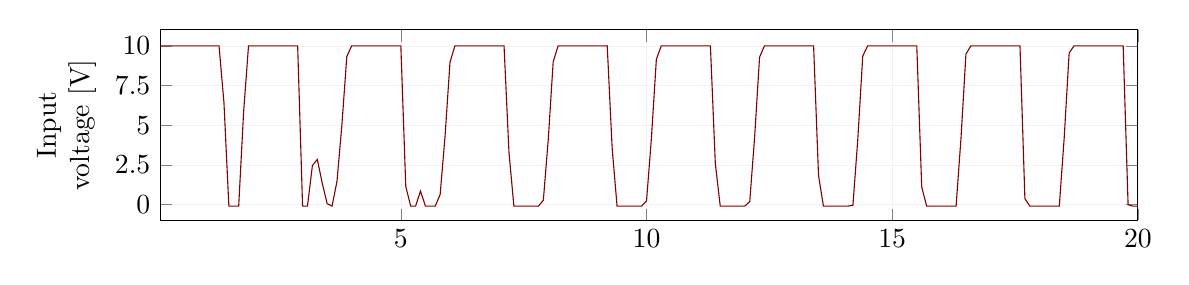
\begin{tikzpicture}
	\begin{axis}[
	ylabel style={align=center},
	ylabel= {Input\\voltage [V]},
	xmin=1, xmax=200,
	ymin=-1, ymax=11,
	legend style={font=\tiny},
	grid=both,
	grid style={line width=.1pt, draw=gray!10},
	width=14cm,height=4cm,
	xticklabels={0,5,10,15,20},xtick={0,50,100,150,200},
	ytick={0,2.5,5,7.5,10},
	%thick
	]
	\addplot[color=Maroon]
	coordinates {
(1,10)(2,10)(3,10)(4,10)(5,10)(6,10)(7,10)(8,10)(9,10)(10,10)(11,10)(12,10)(13,10)(14,6.42235000000000)(15,-0.100000000000000)(16,-0.100000000000000)(17,-0.100000000000000)(18,5.82678000000000)(19,10)(20,10)(21,10)(22,10)(23,10)(24,10)(25,10)(26,10)(27,10)(28,10)(29,9.99284000000000)(30,-0.100000000000000)(31,-0.100000000000000)(32,2.45756000000000)(33,2.84149000000000)(34,1.34924000000000)(35,0.0524647000000000)(36,-0.100000000000000)(37,1.45491000000000)(38,5.00561000000000)(39,9.32467000000000)(40,10)(41,10)(42,10)(43,10)(44,10)(45,10)(46,10)(47,10)(48,10)(49,10)(50,10)(51,1.14491000000000)(52,-0.100000000000000)(53,-0.100000000000000)(54,0.847861000000000)(55,-0.100000000000000)(56,-0.100000000000000)(57,-0.100000000000000)(58,0.632770000000000)(59,4.31874000000000)(60,8.95607000000000)(61,10)(62,10)(63,10)(64,10)(65,10)(66,10)(67,10)(68,10)(69,10)(70,10)(71,10)(72,3.31370000000000)(73,-0.100000000000000)(74,-0.100000000000000)(75,-0.100000000000000)(76,-0.100000000000000)(77,-0.100000000000000)(78,-0.100000000000000)(79,0.271062000000000)(80,4.09422000000000)(81,8.98298000000000)(82,10)(83,10)(84,10)(85,10)(86,10)(87,10)(88,10)(89,10)(90,10)(91,10)(92,10)(93,3.56219000000000)(94,-0.100000000000000)(95,-0.100000000000000)(96,-0.100000000000000)(97,-0.100000000000000)(98,-0.100000000000000)(99,-0.100000000000000)(100,0.226855000000000)(101,4.20206000000000)(102,9.15436000000000)(103,10)(104,10)(105,10)(106,10)(107,10)(108,10)(109,10)(110,10)(111,10)(112,10)(113,10)(114,2.56646000000000)(115,-0.100000000000000)(116,-0.100000000000000)(117,-0.100000000000000)(118,-0.100000000000000)(119,-0.100000000000000)(120,-0.100000000000000)(121,0.180215000000000)(122,4.25729000000000)(123,9.28322000000000)(124,10)(125,10)(126,10)(127,10)(128,10)(129,10)(130,10)(131,10)(132,10)(133,10)(134,10)(135,1.83159000000000)(136,-0.100000000000000)(137,-0.100000000000000)(138,-0.100000000000000)(139,-0.100000000000000)(140,-0.100000000000000)(141,-0.100000000000000)(142,-0.0507925000000000)(143,4.13895000000000)(144,9.35054000000000)(145,10)(146,10)(147,10)(148,10)(149,10)(150,10)(151,10)(152,10)(153,10)(154,10)(155,10)(156,1.11065000000000)(157,-0.100000000000000)(158,-0.100000000000000)(159,-0.100000000000000)(160,-0.100000000000000)(161,-0.100000000000000)(162,-0.100000000000000)(163,-0.100000000000000)(164,4.20404000000000)(165,9.47128000000000)(166,10)(167,10)(168,10)(169,10)(170,10)(171,10)(172,10)(173,10)(174,10)(175,10)(176,10)(177,0.370724000000000)(178,-0.100000000000000)(179,-0.100000000000000)(180,-0.100000000000000)(181,-0.100000000000000)(182,-0.100000000000000)(183,-0.100000000000000)(184,-0.100000000000000)(185,4.20560000000000)(186,9.53644000000000)(187,10)(188,10)(189,10)(190,10)(191,10)(192,10)(193,10)(194,10)(195,10)(196,10)(197,10)(198,-0.0191027000000000)(199,-0.100000000000000)(200,-0.100000000000000)(201,-0.100000000000000)
	};
	
	\end{axis}
	\end{tikzpicture}
	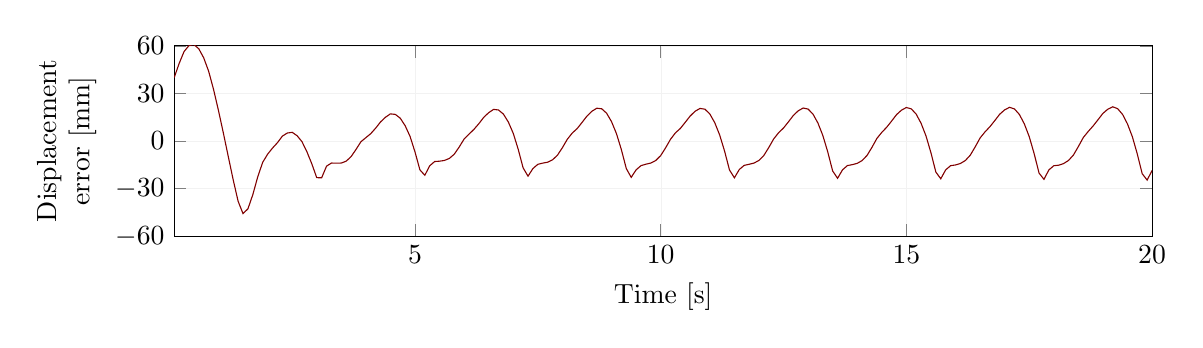
\begin{tikzpicture}
	\begin{axis}[
	ylabel style={align=center},
	ylabel={Displacement\\error [mm]},
	xlabel={Time [s]},
	xmin=1, xmax=200,
	ymin=-60, ymax=60,
	legend style={font=\tiny},
	grid=both,
	grid style={line width=.1pt, draw=gray!10},
	width=14cm,height=4cm,
	xticklabels={0,5,10,15,20},xtick={0,50,100,150,200},
	ytick={-60,-30,0,30,60},
	%thick
	]
	\addplot[color=Maroon]
	coordinates {
(1,40)(2,48.8456000000000)(3,56.3693000000000)(4,60.1398000000000)(5,60.8112000000000)(6,58.1348000000000)(7,52.4454000000000)(8,44.0363000000000)(9,32.5739000000000)(10,19.3014000000000)(11,5.04360000000001)(12,-9.74240000000000)(13,-24.4056000000000)(14,-37.9330000000000)(15,-45.7273000000000)(16,-42.7359000000000)(17,-33.7449000000000)(18,-22.5144000000000)(19,-13.4529000000000)(20,-8.32060000000000)(21,-4.44250000000000)(22,-1.06560000000000)(23,3.06620000000000)(24,5.03320000000000)(25,5.49000000000000)(26,3.38000000000000)(27,-0.403700000000001)(28,-6.73330000000000)(29,-14.3520000000000)(30,-23.0709000000000)(31,-23.1864000000000)(32,-15.8264000000000)(33,-13.8598000000000)(34,-13.9661000000000)(35,-13.8662000000000)(36,-12.6909000000000)(37,-9.80810000000000)(38,-5.27660000000000)(39,-0.429900000000000)(40,2.11050000000000)(41,4.67280000000000)(42,8.13300000000000)(43,12.0687000000000)(44,14.9942000000000)(45,17.1222000000000)(46,16.7835000000000)(47,14.3909000000000)(48,9.64930000000000)(49,2.88970000000001)(50,-6.86760000000000)(51,-18.1614000000000)(52,-21.5778000000000)(53,-15.5874000000000)(54,-12.9258000000000)(55,-12.7027000000000)(56,-12.2236000000000)(57,-10.9370000000000)(58,-8.26200000000000)(59,-3.74980000000000)(60,1.26250000000000)(61,4.36040000000000)(62,7.37070000000000)(63,10.9508000000000)(64,14.9627000000000)(65,17.8894000000000)(66,19.9462000000000)(67,19.5602000000000)(68,16.9537000000000)(69,11.9638000000000)(70,4.81460000000000)(71,-5.16030000000001)(72,-16.8673000000000)(73,-22.1525000000000)(74,-17.3393000000000)(75,-14.6801000000000)(76,-13.9152000000000)(77,-13.3348000000000)(78,-11.8356000000000)(79,-8.89750000000000)(80,-4.18460000000000)(81,1.12260000000000)(82,5.00660000000000)(83,7.83310000000000)(84,11.7306000000000)(85,15.7362000000000)(86,18.7618000000000)(87,20.6751000000000)(88,20.3200000000000)(89,17.4986000000000)(90,12.1998000000000)(91,4.65129999999999)(92,-5.43020000000000)(93,-17.3087000000000)(94,-22.9004000000000)(95,-18.1520000000000)(96,-15.5027000000000)(97,-14.5937000000000)(98,-13.8800000000000)(99,-12.2566000000000)(100,-9.18460000000000)(101,-4.29090000000000)(102,1.09050000000000)(103,5.14920000000000)(104,7.91980000000000)(105,11.8024000000000)(106,15.7492000000000)(107,18.7610000000000)(108,20.5387000000000)(109,20.0728000000000)(110,17.0653000000000)(111,11.5774000000000)(112,3.85990000000000)(113,-6.30700000000000)(114,-18.2253000000000)(115,-23.1715000000000)(116,-17.9254000000000)(117,-15.3333000000000)(118,-14.6479000000000)(119,-13.8789000000000)(120,-12.2000000000000)(121,-9.07340000000000)(122,-4.08900000000000)(123,1.34590000000000)(124,5.22790000000000)(125,8.21060000000000)(126,12.0960000000000)(127,16.1215000000000)(128,19.0671000000000)(129,20.7969000000000)(130,20.1385000000000)(131,16.9439000000000)(132,11.3364000000000)(133,3.49039999999999)(134,-6.86080000000000)(135,-18.8972000000000)(136,-23.4755000000000)(137,-18.1892000000000)(138,-15.4620000000000)(139,-14.8877000000000)(140,-14.0515000000000)(141,-12.2956000000000)(142,-9.05370000000000)(143,-3.95860000000000)(144,1.64890000000000)(145,5.46270000000000)(146,8.70550000000000)(147,12.6013000000000)(148,16.6329000000000)(149,19.4499000000000)(150,21.1197000000000)(151,20.2671000000000)(152,16.9343000000000)(153,11.1370000000000)(154,3.16290000000001)(155,-7.39140000000000)(156,-19.5641000000000)(157,-23.7923000000000)(158,-18.1734000000000)(159,-15.5285000000000)(160,-15.0730000000000)(161,-14.1476000000000)(162,-12.2935000000000)(163,-8.93560000000000)(164,-3.71990000000000)(165,1.91930000000000)(166,5.73350000000000)(167,9.02440000000000)(168,12.8982000000000)(169,16.9134000000000)(170,19.6292000000000)(171,21.2469000000000)(172,20.2185000000000)(173,16.7365000000000)(174,10.8391000000000)(175,2.79740000000001)(176,-7.90880000000001)(177,-20.1860000000000)(178,-24.1418000000000)(179,-18.1977000000000)(180,-15.5726000000000)(181,-15.2237000000000)(182,-14.1973000000000)(183,-12.2436000000000)(184,-8.81910000000000)(185,-3.49290000000000)(186,2.18720000000000)(187,5.99010000000000)(188,9.48700000000000)(189,13.4164000000000)(190,17.4327000000000)(191,20.0549000000000)(192,21.5784000000000)(193,20.3826000000000)(194,16.7604000000000)(195,10.7528000000000)(196,2.62400000000000)(197,-8.22290000000000)(198,-20.6127000000000)(199,-24.6139000000000)(200,-18.5722000000000)
	};
	\end{axis}
	\end{tikzpicture}	
	\caption{Displacement control, 7 kilograms, 3 $\nicefrac{rad}{s}$}
	\label{fig:7kg-3rad}
\end{figure}

\section{Model Predictive Control Development}

A MPC approach has been simulated using an online tool for convex optimization
called CVXGEN~\cite{mattingley2012cvxgen}. This tool allows to write a linear programming
problem description and generate a solver that can be embedded in a Simulink block
for fast and efficient computation. A problem description example for a MPC is
in Figure~\ref{fig:code_example}.

\begin{figure}[H]
	\centering
	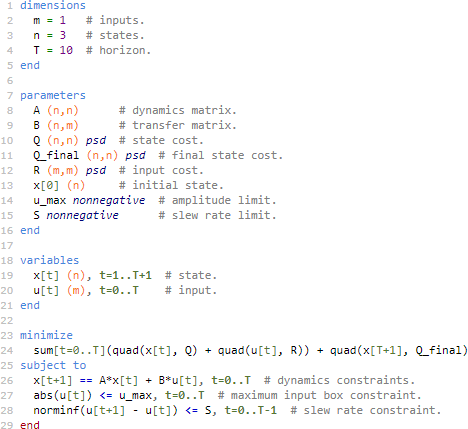
\includegraphics[width=0.8\linewidth]{Images/code_example}
	\caption{MPC problem description example using CVXGEN}
	\label{fig:code_example}
\end{figure}

A prediction horizon of 8 steps has been chosen beforehand. The number of inputs
is one (the voltage), and the system used for control simulation is of the third order.
This has been obtained using the MATLAB System Identification Toolbox 
as for the transfer function described in Chapter~\ref{ch:model}.

However, it appears that the introduction of the hysteresis model
renders the solver unable to solve the minimization problem introduced with
the Model Predictive Control. This is probably due to the fact that
the introduction of the Bouc-Wen model of hysteresis changes the problem
and makes it no more convex. Because of this, the solver generated
by CVXGEN is unable to solve the problem correctly.

For reasons of time, this point has been left as future work.







 % Chapter 6 - Control
\chapter{Conclusions and Future Developments}
\label{ch:conclusion}

McKibben muscles have proven to be of large utility in many fields,
such as rehabilitation, training and actuation of small scale machinery.

The use of tap water as a medium to raise the internal pressure of this kind of muscles
has many advantages: being oil free, they are naturally environment-friendly. Moreover,
the use of water instead of oil makes them safer to use in specific situations.

However, there are drawbacks: water brings problems such as cavitation,
and its lower viscosity makes it harder to control. Furthermore, the McKibben
artificial muscle present a hysteretic behaviour that need to be accounted for
to achieve good control performance.

In this dissertation, the Bouc-Wen model of hysteresis has been proposed
to model the hysteresis of the muscle. This allows to get a very simple,
yet precise model that can be easily controlled using techniques like PID
or MPC control. The Bouc-Wen model has been proposed both in its standard form,
that has been referred as \emph{classic}, and a \emph{generalized} form.
Both versions can express a hysteretic behaviour by use of several
parameters: 4 in case of the classic model, and 8 in case of the generalized one.

Finding these parameters to precisely model a given hysteresis is a hard matter.
While values can be cherry-picked, to achieve highest grades of precision
different methods are needed. In this work, three distinct approaches
have been studied and developed: a Genetic Algorithm, that falls in the category
of Evolutionary Algorithms and that mimics the natural evolution that permeates our world.
Secondly, the Firefly Algorithm that mimics the behaviour of fireflies in the wild,
in its modified version. Lastly, a Particle Swarm Optimization approach where
candidate solutions, called particles, are flown into the solution space and evaluate
it trying to find a global optimum. These last two approaches fall into the category
of Metaheuristic Optimization algorithms.

By using these algorithms it has been showed that it is possible to find parameters
that allow to find a good fit for the hysteresis loop.
Execution times have also been studied to provide a relative rank by timing performance.
This kind of algorithm may be embedded on dedicated hardware
to further speed up the process. This approach may be used
to find parameters for other models and other applications, for example using it
to identify the best gains for a PID controller.

In this work, the control of this type of actuator has been proven to be most effective
with slowly changing reference values. This kind of control may thus be more suitable
for being used in rehabilitation and orthosis, rather than power actuation.

\clearpage

\section{Future Work}

Future work includes:

\begin{itemize}[noitemsep]
	\item Development of Model Predictive Control with the McKibben artificial muscle
	\item Implementation of other Evolutionary Algorithm approaches applied to muscle control
	\item Extension of functionality to the Genetic Algorithm approach to better model the tournament, crossover and mutation steps
	\item Addition of features to the Particle Swarm Optimization approach to attain higher versatility
\end{itemize} % Chapter 7 - Conclusion
\cleardoublepage % Empty page before the start of the next part

%----------------------------------------------------------------------------------------
%	THESIS CONTENT - APPENDICES
%----------------------------------------------------------------------------------------

\appendix

\part{Appendices} % New part of the thesis for the appendix


\lstdefinestyle{mystyle}{
	numbers=left, 
	numberstyle=\tiny, 
	numbersep=8pt, 
	language=Matlab,
	label=glabel
}

\newtcblisting{mylisting}[2][]{
	colframe=Maroon,
	arc=0pt, outer arc=0pt,
	listing only, 
	listing style=mystyle,
	title=#2,
	#1
}



\chapter{Scripts and Algorithms} % Main appendix title
\label{app:algorithms} 

This Appendix contains all scripts and algorithms used for this work.

\section{Scripts}

\subsection{Stair Input Generation}

This script generates the step wave that is to be given as input to the input and output
proportional valves. Given that they have to be symmetric,
the wave given to the output valve is defined as follows.
\begin{align*}
y' = 10 - y
\end{align*}

\begin{mylisting}[hbox,enhanced,drop shadow,label={alg:step_input_generation}]{Stair input generation}
close all
clc
step = 1;	% Volts between two consecutive steps
y = zeros(1,50*10*(1/step));
for v = 0:step:10
	y((v*50)*(1/step)+1:(v+step)*(1/step)*50) = v;
end
y = [y fliplr(y)];
y = [y y y y]';
last = (length(y)-1)/10;
t = (0:0.1:last)';
y = [t y];
\end{mylisting}












 % Appendix A - Scripts
\chapter{The Bouc-Wen Model of Hysteresis}
\label{app:bouc-wen}

A hysteretic semi-physical model has been initially proposed by Bouc
in 1971~\cite{bouc} and subsequently generalized by Wen in 1976~\cite{bouc_wen}.
Since then, it was known as the Bouc-Wen model and 
as been extensively used in the current literature to describe
mathematically components and devices with hysteretic behaviours,
particularly within the areas of civil and mechanical engineering.


\begin{wrapfigure}{l}{0.6\textwidth}
	\centering
	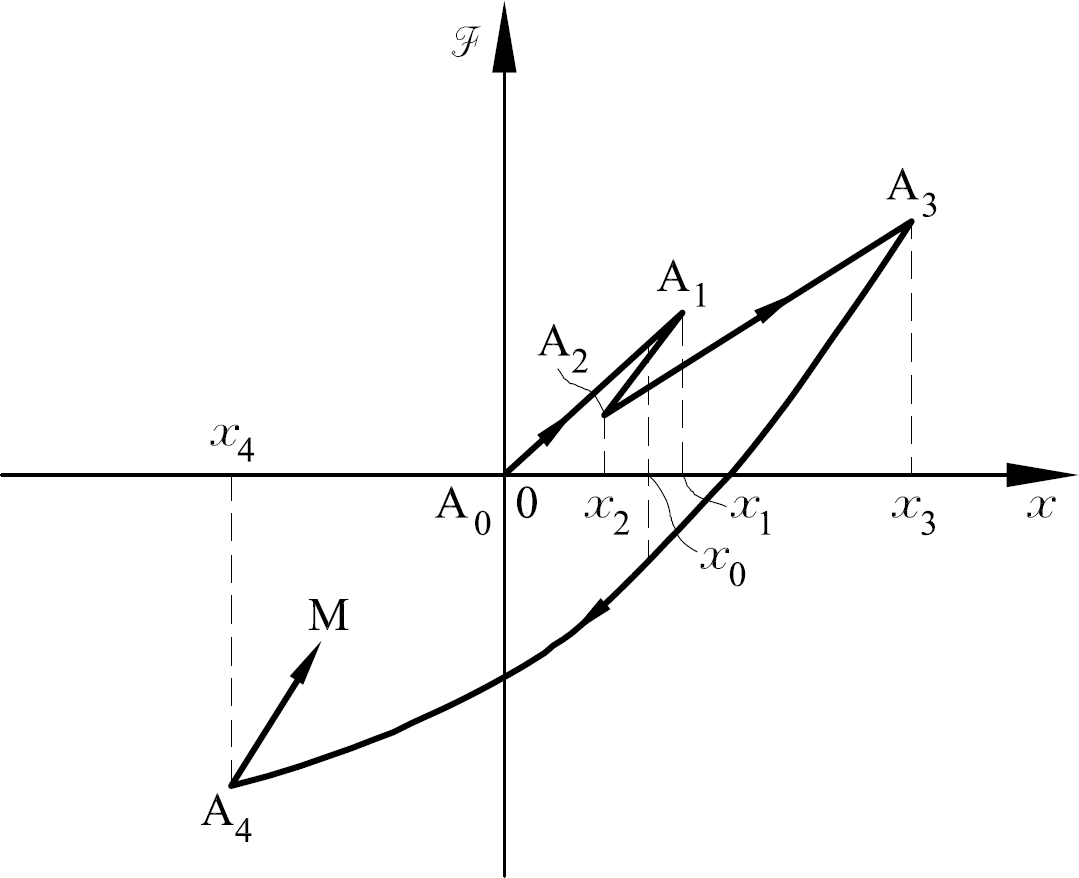
\includegraphics[width=.6\textwidth]{Images/functional}
	\caption{Graph force versus displacement for a hysteresis functional}
	\label{fig:functional}
\end{wrapfigure}

The model consists of a first-order non-linear differential equation
that relates the input displacement to the output restoring
force in a hysteretic way. By choosing a set of parameters
appropriately, it is possible to accommodate the response of
the model to the real hysteresis loops.

In the first paper by Bouc, a functional that describes
the hysteresis phenomenon was proposed. Given $\mathcal{F}$ a force
and $x$ a displacement, from Figure~\ref{fig:functional}
it can be seen that four values of $\mathcal{F}$ correspond
to the single point $x = x_0$. If we consider that $x$ is a function of time,
then the value of the force at instant time $t$ depends not only
from the value of the displacement $x$ at time $t$, but also on past values of $x$.

The following simplifying assumption is made in the original paper.

\newtheorem{assumption1}{Assumption}[chapter]

\begin{assumption1} \label{ass:rip}
The graph of Figure~\ref{fig:functional} remains the same for all
increasing function $x(\cdot)$ between $0$ and $x_1$, for all decreasing
function $x(\cdot)$ between the values $x_1$ and $x_2$, etc.
\end{assumption1}

In current literature, Assumption~\ref{ass:rip} is referred to as
the \emph{rate-independent property}~\cite{visintin2013differential}.
In his paper, Bouc proposes Equation~\ref{eq:functional} as a form for $\mathcal{F}$.

\begin{align} \label{eq:functional}
\frac{d\mathcal{F}}{dt} = g \left(x,\mathcal{F},\sign\left(\frac{dx}{dt}\right)\right)\frac{dx}{dt}.
\end{align}

Consider the equation

\begin{align} \label{eq:functional2}
\frac{d^2x}{dt^2}+\mathcal{F}\left(t\right) = p\left(t\right)
\end{align}

for some given input $p\left(t\right)$ and initial conditions

\begin{align}
\frac{dx}{dt}\left(t_0\right),\qquad x\left(t_0\right)\quad \text{and}\quad \mathcal{F}\left(t_0\right)
\end{align}

at the initial time $t_0$. Equations~\ref{eq:functional} and~\ref{eq:functional2}
describe completely a hysteretic oscillator. Since it is difficult to explicitly
find a solution for Equation~\ref{eq:functional} due to the nonlinearity of the
function $g$, Bouc proposes a variation of the Stieltjes integral to define $\mathcal{F}$:

\begin{align}
\mathcal{F}\left(t\right) = \mu^2x\left(t\right)+\int_\beta^tF\left(V_s^t\right)dx\left(s\right)
\end{align}

where $\beta \in \left[-\inf,+\inf\right)$ is the time instant after which
the displacement and force are defined. $V_s^t$ is the total variation of $x$
in the time interval $\left[s,t\right]$. The function F is chosen so that it
satisfies mathematical properties compatible with the hysteresis. In his work,
Bouc chooses the function F in Equation~\ref{eq:bouc_chosen}:

\begin{align} \label{eq:bouc_chosen}
F\left(u\right)= \sum_{i=1}^N A_i e^{-\alpha_iu},\quad \text{with } \alpha_i > 0
\end{align}

Using this result, Equations~\ref{eq:functional2}--\ref{eq:bouc_chosen}
can be rewritten in the following form.

\begin{align}\label{eq:bouc1}
\frac{d^2x}{dt^2} + \mu^2x + \sum_{i=1}^NZ_i=p\left(t\right)
\end{align}
\begin{align}\label{eq:bouc2}
\frac{dZ_i}{dt} + \alpha_i \left|\frac{dx}{dt}\right|Z_i - A_i\frac{dx}{dt}=0,\quad i=1,\dots,N
\end{align}

Equations~\ref{eq:bouc1} and~\ref{eq:bouc2} are known as the Bouc model.
Equation~\ref{eq:bouc2} has been extended by Wen to describe the restoring
forces with hysteresis in the following form:

\begin{align}
&\dot{z} = A\dot{x} - \alpha\left|\dot{x}\right|z^n - \beta \dot{x}\left|z^n\right| & & \text{for n odd} \label{eq:bw_1} \\
&\dot{z} = A\dot{x} - \alpha\left|\dot{x}\right|z^{n-1}\left|z\right| - \beta \dot{x}z^n & &\text{for n even} \label{eq:bw_2}
\end{align}

Equations~\ref{eq:bw_1} and \ref{eq:bw_2} are the earliest version of what
is known as the Bouc-Wen model of hysteresis.





















 % Appendix B - BW Model

%----------------------------------------------------------------------------------------
%	POST-CONTENT THESIS PAGES
%----------------------------------------------------------------------------------------

% Bibliography

\label{app:bibliography} % Reference the bibliography elsewhere with \autoref{app:bibliography}

\manualmark % Work-around to have small caps also here in the headline
\markboth{\spacedlowsmallcaps{\bibname}}{\spacedlowsmallcaps{\bibname}} % Work-around to have small caps also
%\phantomsection
\refstepcounter{dummy}

\addtocontents{toc}{\protect\vspace{\beforebibskip}} % Place the bibliography slightly below the rest of the document content in the table of contents
\addcontentsline{toc}{chapter}{\tocEntry{\bibname}}

\printbibliography

%----------------------------------------------------------------------------------------

\end{document}
